\chapter{Phonologie}
\label{kap:Phonologie}


In diesem Kapitel geht es weiterhin um lautliche Einheiten der Sprache. Wir untersuchen nun aber deren Funktion innerhalb des Sprachsystems. Phonologische Fragestellungen sind etwa:

\begin{itemize}
\item Warum können wir das Wort \textit{Rat} \textipa{[ra:t]} oder \textipa{[Ka:t]} sprechen, aber nicht \textipa{[ta:t]} oder \textipa{[za:t]}?
\item Warum silbifiziert man \textit{Pal-me} und nicht \textit{Palm-e} oder \textit{Pa-lme}?
\item Warum spricht man im Standarddeutschen \textit{bunt} und \textit{Bund} gleich aus?
\end{itemize}

In Abschnitt~\ref{sec:Allophone} wird zunächst das \is{Phoneminventar}Phoneminventar des Deutschen vorgestellt. Phoneme sind bedeutungsunterscheidene Ab\-straktionen über Sprachlaute. Diese Ab\-straktionen sind unter anderem wichtig für das Verständnis unseres Schriftsystems, weil die alphabetische Komponente unseres Schriftsystems auf den Phonemen basiert (vgl. Kapitel~\ref{kap:Graphematik} zur Graphematik).



In Abschnitt~\ref{subsec:Silbe} wird der Aufbau von Silben beschrieben. Dieser Abschnitt ist ebenfalls essentiell für das Verstehen von Kapitel~\ref{kap:Graphematik}. Aus dem Aufbau der Silbe kann man beispielsweise ableiten, warum \textit{Welle} mit <ll> geschrieben wird, \textit{Welt} aber nicht.

In Abschnitt~\ref{section:phonProzesse} geht es um phonologische Prozesse. Phonologische Prozesse sind sprachspezifische Regeln der Aussprache. Beispielsweise gibt es im Deutschen einen phonologischen Prozess, der dazu führt, dass im Auslaut nie \textipa{[b, d, g, v]} oder \textipa{[z]} gesprochen wird, sondern immer die stimmlosen Partner \textipa{[p, t, k, f]} und \textipa{[s]}, etwa in \textit{Tag} \textipa{[ta:k]} oder \textit{Gras} \textipa{[gKa:s]}. 

Ein in der Forschung sehr präsentes phonologisches Thema, die \is{Merkmalsphonologie}Merkmalsphonologie, ist nicht Teil dieses Kapitels. Wir verzichten bewusst darauf, weil wir uns auf die Aspekte der Phonologie konzentrieren wollen, die für den schulischen Kontext, also beispielsweise das Verständnis für Schreibungen relevant sind. Bei Interesse verweisen wir auf \citet[Kap.4]{Hall2000} oder \citet[19--26]{Wiese2000}.

\section{Phone, Phoneme und Allophone}\label{sec:Allophone}

\is{Phon}Sprachlaute im Allgemeinen nennt man in der Linguistik \textit{Phone}\is{Phon}. Alle Sprachlaute, dazu gehören etwa \textipa{[s, x, i]}, aber auch Schnalzlaute, wie etwa das \textipa{[!]}, welches beispielsweise in der südafrikanischen Sprache !X\'{o}\~o vorkommt,\footnote{siehe Phoneminventare des UCLA phonetics lab archive, \url{http://archive.phonetics.ucla.edu}} sind Phone. Andere Geräusche, wie \zB Fingerschnipsen -- selbst wenn sie kommunikativ gemeint sind -- sind keine Phone \citep[1]{Katamba1996}. Um in der Transkription zu kennzeichnen, dass ein Symbol ein Phon repräsentiert, schreibt man das Symbol in eckige Klammern\is{Transkription!Klammern}, so wie oben  \textipa{[s, x, i]}.

Phonetisch betrachtet sind kaum zwei Produktionen eines Sprachlautes identisch. Sobald unterschiedliche Sprecherinnen oder Sprecher einen Laut, \zB \textipa{[s]}, produzieren, werden diese Produktionen akustisch unterschiedlich sein. Sprecherinnen und Sprecher mit kleineren Vokaltrakten werden etwas höherfrequentes Rauschen produzieren als Personen mit größeren Vokaltrakten. Selbst wenn dieselbe Person einen Laut zweimal produziert, werden die beiden Produktionen akustisch gesehen nicht völlig gleich sein, denn eine Produktion ist vielleicht etwas lauter oder kürzer als die andere. Diese Unterschiede spielen für die Kommunikation aber keine prominente Rolle. Das liegt daran, dass Menschen Ab\-straktionen über Laute bilden, die sie als \gqq{dasselbe} interpretieren. Auch diese Ab\-straktionen werden als Phone bezeichnet. Wenn man etwa drei Produktionen von \textipa{[s]} als \textipa{[s]} transkribiert, nimmt man eine solche Ab\-straktion vor.

Eine höhere Ab\-straktionsebene bilden die sogenannten \textit{Phoneme}\is{Phonem}. Wenn Sprecher unterschiedlicher Dialekte das Wort \textit{Raum} produzieren, sind die Produktionen des r-Lautes zwischen den Sprechergruppen möglicherweise verschieden. Sprecher(innen) des einen Dialekts rollen das r möglicherweise und die anderen produzieren es als Frikativ. Trotzdem interpretieren Hörerinnen und Hörer beide Produktionen als \textit{Raum}, denn für die Bedeutung des Wortes \textit{Raum} sind die Unterschiede irrelevant. Das wäre anders, wenn die Sprecher statt \textipa{[K]} oder \textipa{[r]}  \textipa{[z]} gesagt hätten, denn dieser Unterschied hätte zu einem Bedeutungsunterschied geführt: \textit{Raum -- Saum}. Phone, die bedeutungsunterscheidend sind, werden als \textit{Phoneme} bezeichnet. \textipa{[K]} und \textipa{[z]} sind also Phoneme; die unterschiedlichen Realisierungsvarianten von \textipa{[K]} sind keine Phoneme. Wenn man in der Transkription angeben möchte, dass Laute in der transkribierten Sprache Phoneme sind, notiert man sie in \is{Transkription!Schrägstriche}Schrägstrichen: \textipa{/K/} und \textipa{/z/}.\is{Transkription!Klammern}\is{Transkription!Schrägstriche}

Ob\is{Minimalpaar} zwei Laute Phoneme einer Sprache sind, stellt man über eine \textit{Minimalpaaranalyse}\is{Minimalpaaranalyse} fest \citep[22--23]{Katamba1996}. Ein Minimalpaar sind zwei Wörter, die sich in genau einem Laut unterscheiden, etwa \textit{Deich} \textipa{[d\t*{aI}\c{c}]} und \textit{Teich} \textipa{[t\t*{aI}\c{c}]}. Wenn durch den lautlichen Unterschied ein Bedeutungskontrast hergestellt wird, handelt es sich bei den Lauten um Phoneme der jeweiligen Sprache.


\begin{Definition}{Phonem}\label{def:Phonem}\is{Phonem}\\
\noindent
Phoneme sind die kleinsten bedeutungsunterscheidenden\is{bedeutungsunterscheidend} Einheiten einer Sprache. Man ermittelt sie durch Minimalpaaranalyse\is{Minimalpaaranalyse}. In der Transkription können sie zwischen \is{Transkription!Schrägstriche}Schrägstriche geschrieben werden. 

\end{Definition}

Im Folgenden betrachten wir einige Beispiele für Minimalpaare. Wir beginnen mit \textit{Fass} \textipa{[fas]} und \textit{das} \textipa{[das]} in Beispiel~(\ref{ea:Fassdas}). Die beiden Wörter unterscheiden sich nur in einem einzigen Laut, haben aber unterschiedliche Bedeutung. Daraus kann man ableiten, dass die beiden Laute, die den Bedeutungskontrast produzieren, also \textipa{/f/} und \textipa{/d/} im Deutschen Phoneme sind.

Beispiel~(\ref{ex:MitteMotte}) zeigt einen vokalischen Kontrast: \textit{Mitte} \textipa{[\textprimstress mI\.*t@]} und \textit{Motte} \textipa{[\textprimstress mO\.*t@]} unterscheiden sich nur durch den ersten Vokal. Da auch diese beiden Wörter nicht bedeutungsgleich sind, kann man schlussfolgern, dass \textipa{/I/} und \textipa{/O/} Phoneme des Deutschen sind.


Grundlage für die Ermittlung von Phonemen ist immer die Lautung, nicht die Schreibung. So zeigt Beispiel~(\ref{ex:Schal-Saal}), dass \textipa{/S/} und \textipa{/z/} Phoneme sind, denn lautlich unterscheiden sich die Wörter \textit{Schal} und \textit{Saal} nur im Anlaut, obwohl die Schreibung mehrere Unterschiede aufweist.

Auch \textit{Ruhm} \textipa{[ru:m]} (mit Zungenspitzen-r) und \textit{Ruhm} \textipa{[Ku:m]} (mit uvularem \textipa{[K]}) in Beispiel~(\ref{ex:Ruhm}) bilden ein Minimalpaar\is{Minimalpaar}, da sie sich ebenfalls nur in einem einzigen Laut unterscheiden. Im Unterschied zu den vorangegangenen Beispielen haben die beiden Äußerungen jedoch dieselbe Bedeutung. 
Aus diesem Minimalpaar kann man deshalb nicht ableiten, dass \textipa{[r]} und \textipa{[K]} Phoneme sind, weil die unterschiedlichen Laute nicht dazu beitragen, dass ein Bedeutungskontrast hergestellt wird. Solche Phone, die keinen Bedeutungskontrast herstellen können, nennt man \textit{Allophone}\is{Allophon} eines Phonems. Allophone eines Phonems können Bedeutungskontraste mit anderen Phonemen herstellen, aber nicht mit anderen Allophonen desselben Phonems.


\ea \label{ea:Minimalpaaranalyse}
\ea \label{ea:Fassdas} \textit{Fass} \textipa{[fas]} -- \textit{das} \textipa{[das]}: Bedeutungskontrast, d.\,h. \textipa{/f/} und \textipa{/d/} sind Phoneme des Deutschen.
\ex \label{ex:MitteMotte} \textit{Mitte} \textipa{[\textprimstress mI\.*t@]} -- \textit{Motte} \textipa{[\textprimstress mO\.*t@]}: Bedeutungskontrast, d.\,h. \textipa{/I/} und \textipa{/O/} sind Phoneme des Deutschen.
\ex \label{ex:Schal-Saal} \textit{Schal} \textipa{[Sa:l]} -- \textit{Saal} \textipa{[za:l]}: Bedeutungskontrast, d.\,h. \textipa{/S/} und \textipa{/z/} sind Phoneme des Deutschen.
\ex \label{ex:Ruhm} \textit{Ruhm} \textipa{[ru:m]} -- \textit{Ruhm} \textipa{[Ku:m]}: kein Bedeutungskontrast, d.\,h. \textipa{[r]} und \textipa{[K]} sind keine Phoneme des Deutschen, sondern Allophone des \textipa{/K/}-Phonems.
\z 
\z 



Allophone sind \textit{Varianten eines Phonems}. Alle physikalisch unterschiedlichen Realisationen eines Lautes, die einem einzigen Phonem zugeordnet werden, zählen als Allophone dieses Phonems \citep[18]{Katamba1996}. \is{r-Varianten}Die Laute \textipa{[r, \;R, K]} sind Allophone des Phonems \textipa{/K/}.\footnote{Prinzipiell könnte man jede der r-Varianten als Phonem der r-Allophone ansehen. Wir nehmen hier \textipa{/K/} als Phonem an, weil es verglichen mit den anderen Varianten die größte Verbreitung hat \citep[52]{DudenAussprache2023}.} Da Sprecherinnen und Sprecher zwischen den drei \textipa{/K/}-Lauten prinzipiell frei wählen können, welche der Varianten sie benutzen wollen, spricht man von \is{Allophon!frei}\textit{freien Allophonen} \citep[42--43]{Ramers1998}.

Für den Status als Allophon ist es egal, ob ein lautlicher Unterschied salient ist oder nicht. Wenn man zum Beispiel die Wörter \textit{küssen} und \textit{Kuss} produziert, unterscheiden sich die Artikulationsstellen der beiden \textipa{/k/}-Laute: Da dem \textipa{[k]} bei \textit{küssen} ein Vorderzungenvokal folgt, wird das \textipa{[k]} weiter vorne produziert als bei \textit{Kuss}, wo dem \textipa{[k]} ein Hinterzungenvokal folgt.\footnote{Deutlicher ist der Unterschied, wenn man \textipa{[ki]} und \textipa{[ku]} vergleicht.} Dieser Unterschied ist den meisten Hörerinnen und Hörern gar nicht bewusst; trotzdem zählen die beiden Realisierungsvarianten des \textipa{/k/} als Allophone. Anders als bei den \textipa{/K/}-Allophonen handelt es sich bei dieser Allophonie jedoch nicht um eine freie Allophonie, da die Realisierung von der lautlichen Umgebung abhängt. Solche Allophone bezeichnet man als\is{Allophon!stellungsbedingt}\is{Allophon!komplementär} \textit{stellungsbedingte} oder \textit{komplementäre Allophone} von \textipa{/k/}. Der Begriff \textit{komplementär} ist darauf zurückzuführen, dass ein Allophon, welches in einer Position vorkommt, \zB vor Vorderzungenvokalen, nicht in der anderen vorkommen kann, also vor Hinterzungenvokalen (\cite[38--39]{Hall2000}, \cite[46--49]{Ramers1998}, \cite[18]{Lass2000}).


Als nächstes werden die Laute \textipa{[\c{c}, x, X]} betrachtet, die in \textit{Fichte} \textipa{[\textprimstress fI\c{c}.t@]}, \textit{suchte} \textipa{[\textprimstress zu:x.t@]} und \textit{dachte} \textipa{[\textprimstress daX.t@]} vorkommen. Um zu überprüfen, ob diese Laute Phoneme des Deutschen sind, bildet man Minimalpaare:
\ea
\ea mich \textipa{[mI\c{c}]} -- mit \textipa{[mIt]}
\ex hoch \textipa{[ho:x]} -- Hof \textipa{[ho:f]}
\ex Dach \textipa{[daX]} -- das \textipa{[das]}
\z
\z
Die Laute kontrastieren also mit anderen Phonemen des Deutschen. Es gibt jedoch keine Minimalpaare, wo \textipa{[\c{c}, x, X]} miteinander kontrastieren. Ein solches Minimalpaar ist auch gar nicht möglich, weil die Laute, wie in Abschnitt~\ref{subsubsection:Frikative} beschrieben, in \textit{komplementärer Distribution} stehen. Der Kontext bestimmt also, welcher der drei Laute gesprochen wird: Nach Konsonanten, Vorderzungenvokalen und morpheminitial spricht man \textipa{[\c{c}]}, nach \textipa{/u/} und \textipa{/o/} spricht man \textipa{[x]} und nach allen anderen Vokalen \textipa{[X]} (\citet[192]{Pompino-Marschall2020}). \textipa{[\c{c}, x, X]} sind also komplementäre Allophone eines einzigen Phonems. \citet[63--64]{Hall2000} nimmt als Phonem dieser Allophone das \textipa{/\c{c}/} an, weil es in den meisten Kontexten vorkommt.


\begin{Definition}{Allophone}\\
\noindent
Allophone sind Realisierungsvarianten eines Phonems. In der Transkription werden sie in eckige Klammern geschrieben.\is{Transkription!Klammern} 

\end{Definition}


Ein Phonem ist immer ein Phonem einer bestimmten Sprache. Man kann also nicht generell sagen, \textipa{/s/} und \textipa{/z/} seien Phoneme, sondern nur: \textipa{/s/} und \textipa{/z/} sind Phoneme \textit{des Deutschen}, weil sie im Deutschen bedeutungsunterscheidend sind. Im Mandarin beispielsweise sind diese Laute nicht bedeutungsunterscheidend.

Um\is{Minimalpaar} zu belegen, dass ein Laut phonemisch ist, genügt ein einziges Minimalpaar. Einen ganz bestimmten Kontrast muss man nur finden, wenn man nachweisen will, dass zwei bestimmte Laute keine Allophone in der jeweiligen Sprache sind. Das Minimalpaar \textit{Teich--Deich} belegt beispielsweise, dass \textipa{/t/} und \textipa{/d/} Phoneme sind; man muss \textipa{/t/} nicht noch mit \textipa{/z/, /b/} oder anderen Lauten kontrastieren, es sei denn, man vermutet, sie könnten Allophone eines einzigen Phonems sein. Zur Überprüfung des Phonemstatus ist es auch nicht notwendig, Laute desselben Artikulationsmodus zu kontrastieren. In \textit{Topf} \textipa{/tO\t{pf}/} und \textit{toll} \textipa{/tOl/} kontrastieren die Phoneme \textipa{/\t{pf}/} und \textipa{/l/}, also eine Affrikate mit einem Lateral. Man zeigt damit, dass \textipa{/\t{pf}/} und \textipa{/l/} Phoneme des Deutschen sind. Das Beispiel zeigt auch, dass die zu kontrastierenden Laute nicht zwangsläufig am Wortanfang stehen müssen.

Wie schon angesprochen ist es bei der Minimalpaaranalyse wichtig, dass der Vergleich aufgrund der Lauteigenschaften des Wortes, nicht aufgrund der Orthografie erfolgt: \textit{Rad} \textipa{[Ka:t]} -- \textit{Rat} \textipa{[Ka:t]} ist kein Minimalpaar, aus welchem man schlussfolgern kann, dass \textipa{/d/} und \textipa{/t/} Phoneme sind, denn die beiden Wörter kontrastieren nur in der Schreibung und nicht in der Lautung. Genauso kann man aus \textit{Wahl} \textipa{[va:l]} -- \textit{Wal} \textipa{[va:l]} nicht schlussfolgern, dass \textipa{/h/} ein Phonem ist, denn das h in \textit{Wahl} wird nicht gesprochen. Aus \textit{Weg} \textipa{[ve:k]} und \textit{weg} \textipa{[vEk]} kann man hingegen schlussfolgern, dass \textipa{/e:/} und \textipa{/E/} Phoneme sind, selbst wenn die Wörter sich orthografisch nur durch den Großbuchtstaben bei \textit{Weg} unterscheiden.

Es gibt einige Laute, deren phonemischer Status umstritten ist. Dazu gehört der \is{Laute!Knacklaut}Knacklaut \textipa{[P]} (vgl. Abschnitt~\ref{subsection:Plosive}), außerdem noch \textipa{[\t{dZ}, Z]} und \textipa{[N]}, die Vokale insgesamt und im Besonderen \textipa{[E:, @, 5]}. Argumente für und gegen ihren phonematischen Status finden Sie in Exkurs~\ref{Exkurs:Knacklaut}.


\begin{Exkurs}{Laute, deren Phonemstatus umstritten ist}\label{Exkurs:Knacklaut}


Für einige Laute kann man zwar Minimalpaare finden, es spricht aber trotzdem einiges dagegegen, sie als Phoneme des Deutschen aufzufassen. Einer dieser Laute ist der Knacklaut. Es gibt Minimalpaare, bei denen der Knacklaut mit einem Phonem des Deutschen kontrastiert, etwa \textit{aus} \textipa{[PaUs]} und \textit{Haus} \textipa{[haUs]}, \textit{Elle} \textipa{[\textprimstress PE\.*{l}@]} -- \textit{Welle} \textipa{[\textprimstress vE\.*{l}@]}, \textit{Ohr} \textipa{[Po:5]}-- \textit{Tor} \textipa{[to:5]}, \textit{vereisen} \textipa{[f5\textprimstress P\t*{aI}.z\s{n}]} -- \textit{verreisen} \textipa{[f5\textprimstress K\t*{aI}.z\s{n}]}. Für \citet[40]{NoackPhonologie2016} ist die Existenz solcher Minimalpaare ausreichend, um den Knacklaut als Phonem zu betrachten.

Die meisten Phonologinnen und Phonologen -- \zB \citet{RamersVater1991}, \citet{Ramers1998}, \citet{Hall2000}, \citet{Ternes2012}, \citet{FuhrhopPeters2013} -- argumentieren aber gegen den phonematischen Status des Knacklauts. Dabei werden vor allem zwei Argumente bemüht. Das erste Argument ist, dass die Position des Knacklautes vorhersagbar ist (vgl. Abschnitte~\ref{subsection:Plosive} und \ref{sec:Epenthese}), und das zweite, dass der Knacklaut in fließender Rede an prinzipiell jeder Stelle entfallen kann. Beides ist bei anderen Phonemen nicht der Fall.

Bezüglich des ersten Arguments führt \citet[65--66]{Hall2000} aus, dass die Positionierung des Knacklauts klaren Regeln folgt und somit -- im Gegensatz zur Positionierung aller anderen Phoneme -- vorhersagbar ist. Er steht im Onset von betonten Silben oder wortinitial, wenn der Onset sonst leer wäre. Für kein anderes Phonem ist mittels einer solchen Regel voraussagbar, wo es steht.

In Bezug auf das zweite Argument untersuchte \citet{Krech1968} den Gebrauch des glottalen Verschlusslautes bei Berufssprechern und stellte fest, dass er abhängig vom Sprechtempo und der lautlichen Umgebung entfallen kann. \citet[96]{RamersVater1991} schlussfolgern daraus, dass der Knacklaut deshalb nicht zugrundeliegend sein kann und folglich kein Phonem ist. 

Die\is{Laute![ʒ]}\is{Laute![d͡ʒ]} postalveolaren stimmhaften Laute \textipa{/Z/} wie in \textit{Journal} und \textipa{/\t{dZ}/} wie in \textit{Dschungel} führt \citet[68]{Hall2000} als Phoneme auf, obwohl sie nur in Fremdwörtern vorkommen. Hall argumentiert, dass Laute, die in einer Sprache echt fremdsprachlich sind, von den Sprecherinnen und Sprechern in der Regel durch native Laute ersetzt werden. Ein Beispiel ist die th-Ausprache durch deutschen Muttersprachler in englischen Fremdwörtern. Die Laute \textipa{[T, D]} werden dabei durch \textipa{[s, z]} ersetzt \zB in \textit{Think tank, Motherboard}. Hall argumentiert, dass diese Ersetzungen bei \textipa{/Z/} und \textipa{/\t{dZ}/} nicht vorkommen und die Laute deshalb zum deutschen Phoneminventar gezählt werden müssten. 

Auch der phonemische Status des velaren Nasals ist umstritten. Zwar gibt es Minimalpaare wie \textit{Wanne} \textipa{[\textprimstress va\.*n@]} -- \textit{Wange} \textipa{[\textprimstress va\.*N@]} \citep[63]{FuhrhopPeters2013}. Der Laut kommt aber sehr eingeschränkt vor, nämlich nur nach ungespannten Vokalen. Außerdem kann man sein Vorkommen \citet[66f]{Hall2000} zufolge immer als Resultat einer Assimilation erklären (vgl. Abschnitt~\ref{subsection:Assimilation}).

Bei den Vokalen argumentiert \citet[68--70]{Hall2000} dafür, dass \textipa{/i:, I, y:, Y, e:, E:, E, a:, a u:, U, o:, O, \o:, \oe/} und \textipa{/@/} \is{Laute!Schwa}Phoneme des Deutschen sind. Er betrachtet also die gespannten Langvokale und die ungespannten Vokale als Phoneme. Die kurzen gespannten Vokale \textipa{[i, y, e, u, o, \o]} sind Hall zufolge keine Phoneme, denn sie sind vorhersagbar: Wenn ein gespannter Vokal in unbetonter Position steht, wird er gekürzt. Da die Länge vom Kontext abhängig ist, sind Minimalpaare ausgeschlossen.

Aufgrund von Oppositionen wie \textit{sehen -- säen} nimmt Hall, genauso wie das \citet{DudenAussprache2023}, ein Phonem \textipa{/E:/} neben \textipa{/E/} und \textipa{/e:/} an. In Abschnitt~\ref{subsection:Gespanntheit} wurde jedoch diskutiert, dass \textipa{[E:]} sehr selten ist und -- außer in kontrastiven Kontexten -- durch \textipa{[e:]} ersetzt wird, was den phonematischen Status von \textipa{[E:]} infrage stellt.

Sehr problematisch ist auch der Status von \textipa{[@]}. Das Problem bei diesem Laut ist, dass er nur in unbetonter Silbe vorkommt und die Möglichkeiten für die Bildung von Minimalpaaren sehr eingeschränkt sind. \citet[70]{Hall2000} zufolge sollte der Schwa-Laut als Phonem betrachtet werden, da er mit anderen Vokalen kontrastiert. Als Beispiel nennt er das Wortpaar \textit{genau -- genial}. Dagegen lässt sich einwenden, dass dieses Beispiel kein Minimalpaar ist, weil es sich nicht durch nur einen einzigen Laut unterscheidet. \citet[59]{FuhrhopPeters2013} stellen fest, dass sich Schwa wie ein Phonem verhält und nennen die Minimalpaare \textit{Motte -- Motto} und \textit{gerannt -- Garant}. Sie argumentieren aber für einen besonderen Status von Schwa. Als ein Argument für diesen besonderen Status von Schwa innerhalb der deutschen Vokale führen sie die Schwa-Tilgung an. Bei dem Minimalpaar \textit{Hirten -- Hirtin} kann das Schwa bei \textit{Hirten} getilgt werden, das \textipa{/I/} bei \textit{Hirtin} aber nicht. 

Der Schwa-Laut kontrastiert sehr häufig mit dem tiefen Schwa. Das \citet[35]{DudenAussprache2023} nennt \textit{Neue -- Neuer} als Minimalpaar. Weitere Beispiele sind \textit{Messe -- Messer, Lehre -- Lehrer}. Wenn man diese Wortpaare als Minimalpaare akzeptiert, müsste man auch das tiefe Schwa als Phonem ansehen. Das tut Hall nicht und begründet das damit, dass das tiefe Schwa ein -- stellungsbedingtes -- Allophon des Phonems \textipa{/K/} sei: Wenn \textipa{/K/} in der Koda einer Silbe steht, wird es \textipa{[5]} gesprochen. Auch das \citet[35]{DudenAussprache2023} und \citet[58f]{FuhrhopPeters2013} geben den tiefen Schwa-Laut als \textipa{/K/}-Allophon an. 




\end{Exkurs}



Wenn man für alle in einer Sprache vorkommenden Laute Minimalpaaranalysen durchführt, ermittelt man das\is{Phoneminventar} \textit{Phoneminventar} dieser Sprache. In Tabelle~\ref{tab:IPA_Kons_Phoneme} ist das konsonantische Phoneminventar des Deutschen nach \citet{Hall2000} dargestellt. Als Phonem für die r-Allophone ist bei Hall \textipa{/\textscr/} angegeben, wir wählen hier das häufigere \textipa{/K/}. Abbildung~\ref{fig:Vokalviereck_phonemisch} stellt die phonemischen Vokale dar. Tabelle~\ref{tab:Phoneminventar} enthält Minimalpaare, die den Phonemstatus der einzelnen Laute belegen. 



\begin{table}
    \centering
\caption{\label{tab:IPA_Kons_Phoneme} Konsonantische Phoneme des Deutschen angelehnt an \citet[62]{Hall2000}. Spalten: Artikulationsorte. Zeilen: Artikulationsarten: Stimmlose Konsonanten stehen links in einer Zelle, stimmhafte stehen rechts.}

% \fittable
{
\begin{tabular}{l @{~}l@{~}l@{}l  @{~~~~~~} l@{}l@{}l  @{~~~~~~} l@{~}l@{}l  @{~~~~~~} l@{~}l@{}l @{~~~~~~} l@{~}l@{}l  @{~~~~~~} l@{~}l@{}l @{~~~~}  l @{~~~~} l }
\lsptoprule
&\multicolumn{2}{c}{\rotatebox{90}{bilabial}} &&\multicolumn{2}{c}{\rotatebox{90}{labiodental}} && \multicolumn{2}{c}{\rotatebox{90}{alveolar}} && \multicolumn{2}{c}{\rotatebox{90}{postalveolar}} && \multicolumn{2}{c}{\rotatebox{90}{palatal}} && \multicolumn{2}{c}{\rotatebox{90}{velar}} && {\rotatebox{90}{uvular}} &  {\rotatebox{90}{glottal}}\\
\midrule
Plosive& \textipa{p}& \textipa{b} & &&&  & \textipa{t} &\textipa{d}&  &&& & & & & \textipa{k} &\textipa{g} \\
Affrikaten&&& & \textipa{\t{pf}}& && \textipa{\t{ts}} &&& \textipa{\t{tS}} & \textipa{\t{dS}}  \\
Frikative &&&& f & v && s & z & &\textipa{S} &  \textipa{Z} && \textipa{\c{c}} &&& &&&   \textipa{\textinvscr}& \textipa{h}\\
Nasale && \textipa{m} && &&&& \textipa{n} &&&& & && &&\textipa{N} \\
Approximanten && & & & &&&&&&&&& \textipa{j} \\
Laterale && && &&&& \textipa{l}       \\
\lspbottomrule
\end{tabular}
}
\end{table}






\begin{figure}
    \centering
    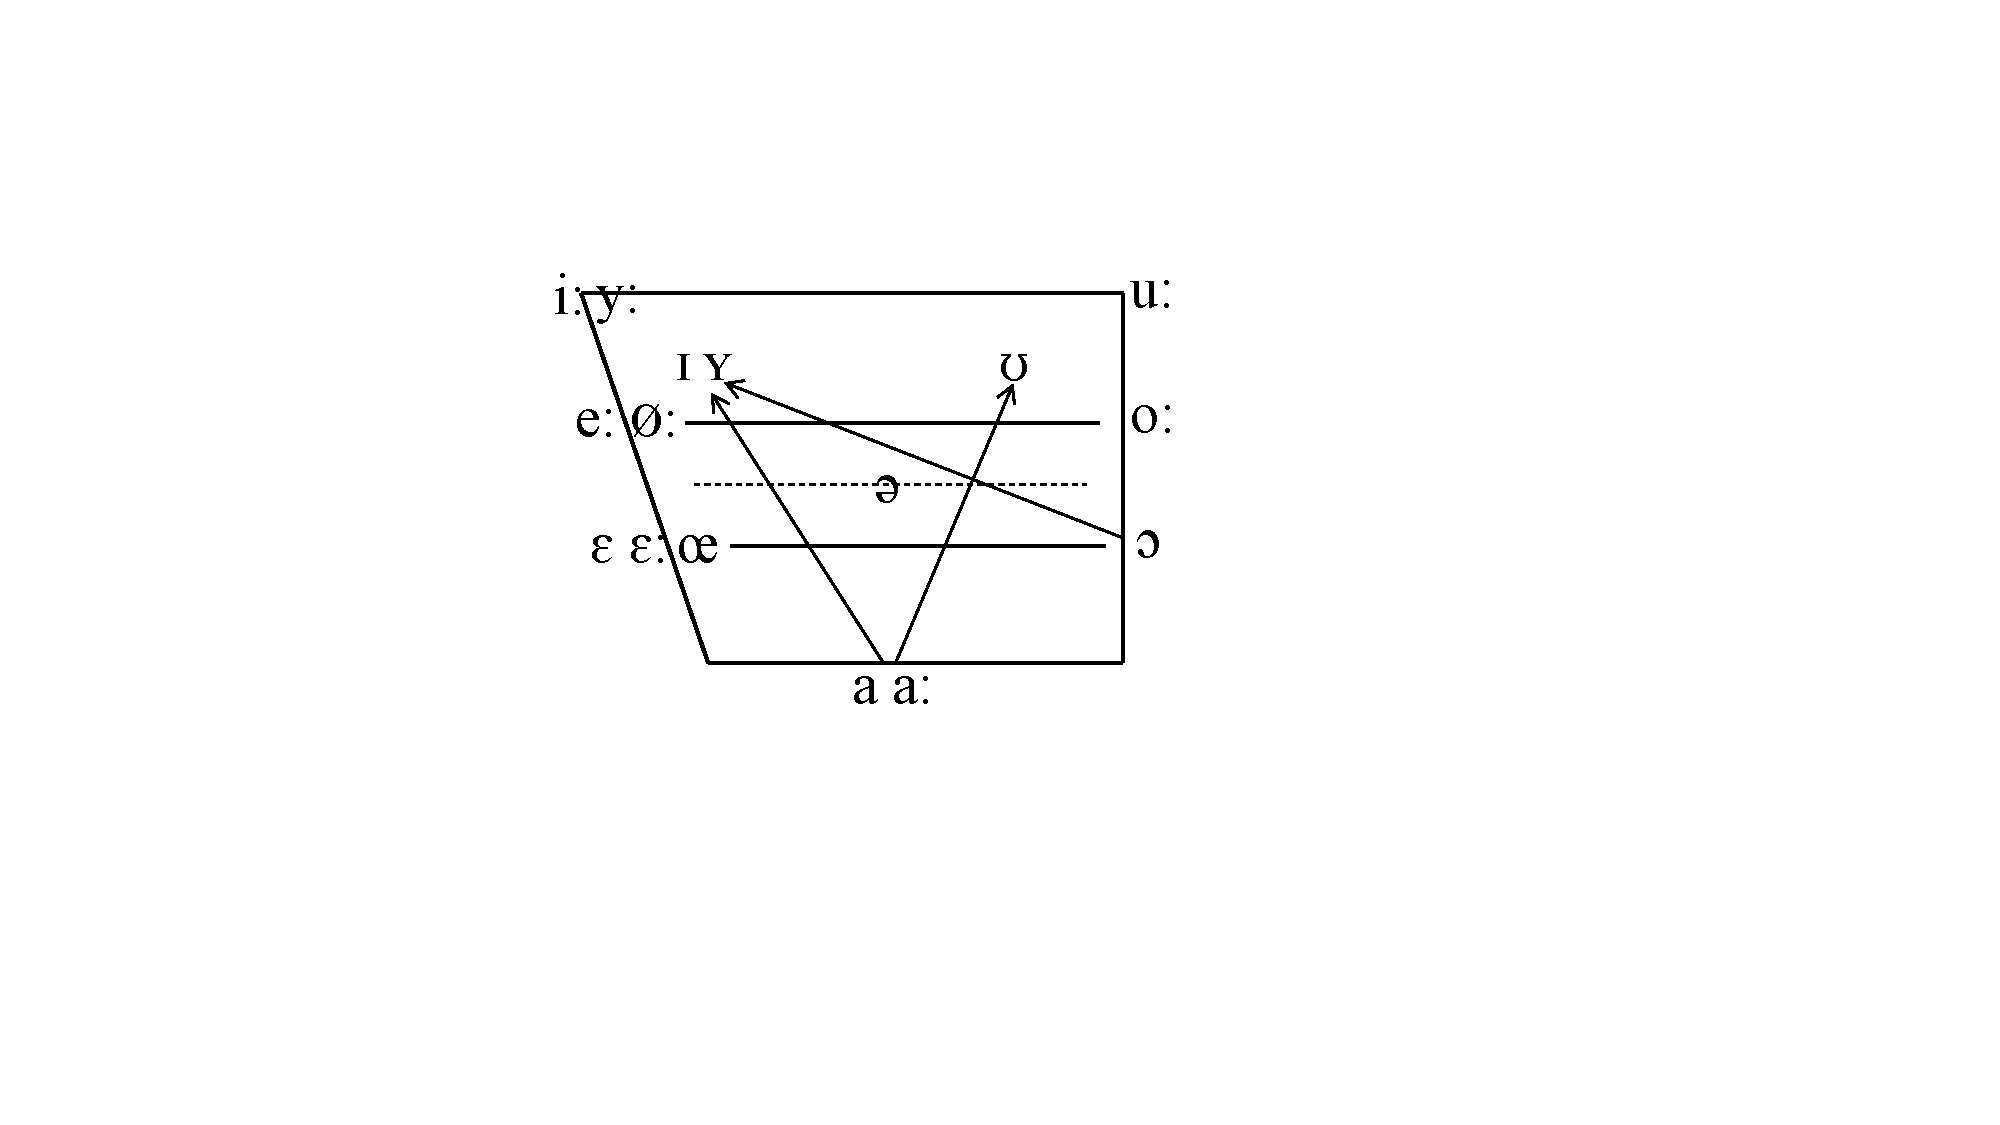
\includegraphics[width=.5\textwidth]{figures/Vokalviereck_Phoneme.pdf}
    \caption{Phonemische deutsche Vokale nach \citet{Hall2000}.\label{fig:Vokalviereck_phonemisch}}
\end{figure}


\begin{table}
\centering
\footnotesize
\caption{Phoneminventar des Deutschen angelehnt an \citet[62, 68]{Hall2000}\label{tab:Phoneminventar}}
\resizebox{\textwidth}{!}{
\begin{tabular}{llll}\lsptoprule
Phonem & Minimalpaar&Phonem & Minimalpaar\\\midrule
\textipa{/p/} & \textit{Pein} \textipa{[p\t*{aI}n]} -- \textit{Bein} \textipa{[b\t*{aI}n]} & \textipa{/a/}& \textit{Bann} \textipa{[ban]} -- \textit{Bahn} \textipa{[ba:n]} \\
\textipa{/b/} & \textit{Bein} \textipa{[b\t*{aI}n]} -- \textit{kein} \textipa{[k\t*{aI}n]} & \textipa{/a:/}& \textit{Rasen} \textipa{[Ka:.z@n]} -- \textit{Rosen} \textipa{[Ko:.z@n]} \\
\textipa{/t/} & \textit{Teich} \textipa{[t\t*{aI}\c{c}]} -- \textit{Deich} \textipa{[d\t*{aI}\c{c}]} & \textipa{/i:/}& \textit{Miete} \textipa{[\textprimstress mi:.t@]} -- \textit{Mitte} \textipa{[\textprimstress mI\.*{t}@]} \\
\textipa{/d/} & \textit{schade} \textipa{[\textprimstress Sa:.d@]} -- \textit{Schale} \textipa{[\textprimstress Sa:.l@]} & \textipa{/I/}& \textit{Mitte} \textipa{[\textprimstress mI\.*t@]} -- \textit{Motte} \textipa{[\textprimstress mO\.*t@]} \\
\textipa{/k/} & \textit{Ecke} \textipa{[\textprimstress PE\.*k@]} -- \textit{Egge} \textipa{[\textprimstress PE\.*g@]} & \textipa{/y:/}& \textit{wühlen} \textipa{[\textprimstress vy:.l@n]} -- \textit{Wahlen} \textipa{[\textprimstress va:.l@n]} \\
\textipa{/g/} & \textit{Geiz} \textipa{[g\t*{aI}\t{ts}]} -- \textit{Reiz} \textipa{[K\t*{aI}\t{ts}]} & \textipa{/Y/}& \textit{Hütte} \textipa{[\textprimstress hY\.*{t}@]} -- \textit{Hüte} \textipa{[\textprimstress hy:.t@]} \\
\textipa{/\t{pf}/} & \textit{Topf} \textipa{[tO\t{pf}]} -- \textit{toll} \textipa{[tOl]} & \textipa{/u:/} & \textit{gut} \textipa{[gu:t]} -- \textit{Gott} \textipa{[gOt]}\\
\textipa{/\t{ts}/} & \textit{Zopf} \textipa{[\t{ts}O\t{pf}]} -- \textit{Topf} \textipa{[tO\t{pf}]} & \textipa{/U/} &\textit{Butter} \textipa{[\textprimstress bU\.*{t}5]} -- \textit{bitter} \textipa{[\textprimstress bI\.*{t}5]}\\
\textipa{/\t{tS}/} & \textit{Kutsche} \textipa{[\textprimstress kU\.*{\t{tS}}@]} -- \textit{Kuppe} \textipa{[\textprimstress kU\.*{p}@]}& \textipa{/e:/} & \textit{beten} \textipa{[\textprimstress be:.t@n]} -- \textit{Betten} \textipa{[\textprimstress bE\.*{t}@n]}\\
\textipa{/\t{dZ}/}& \textit{Gin} \textipa{[\t{dZ}In]} -- \textit{Kinn} \textipa{[kIn]} & \textipa{/E/} & \textit{Welt} \textipa{[vElt]} -- \textit{Wald} \textipa{[valt]}\\
\textipa{/f/} & \textit{fein} \textipa{[f\t*{aI}n]} -- \textit{Wein} \textipa{[v\t*{aI}n]} &\textipa{/E:/} & \textit{säen} \textipa{[\textprimstress zE:.@n]} -- \textit{sehen} \textipa{[\textprimstress ze:.@n]}\\
\textipa{/v/} & \textit{Wein} \textipa{[v\t*{aI}n]} -- \textit{kein} \textipa{[k\t*{aI}n]} &\textipa{/o:/} & \textit{Ofen} \textipa{[\textprimstress Po:.f@n]} -- \textit{offen} \textipa{[\textprimstress PO\.*{f}@n]}\\
\textipa{/s/} & \textit{Masse} \textipa{[\textprimstress ma\.*s@]} -- \textit{Masche} \textipa{[\textprimstress ma\.*S@]} & \textipa{/O/} & \textit{locker} \textipa{[\textprimstress lO\.*k5]} -- \textit{lecker} \textipa{[\textprimstress lE\.*k5]}\\
\textipa{/z/} & \textit{Besen} \textipa{[\textprimstress be:.z@n]} -- \textit{beten} \textipa{[\textprimstress be:.t@n]} & \textipa{/\o:/}& \textit{Böden} \textipa{[\textprimstress b\o:.d@n]} -- \textit{Boden} \textipa{[\textprimstress bo:.d@n]}\\
\textipa{/S/} & \textit{Schuh} \textipa{[Su:]} -- \textit{Kuh} \textipa{[ku:]} & \textipa{/\oe/}& \textit{löschen} \textipa{[\textprimstress l\oe \.*S@n]} -- \textit{Laschen} \textipa{[\textprimstress la\.*S@n]}\\
\textipa{/Z/} & \textit{Jacques} \textipa{[Zak]} -- \textit{Pack} \textipa{[pak]} &\textipa{/@/} & \textit{Motte} \textipa{[\textprimstress mO\.*{t}@]} -- \textit{Motto} \textipa{[\textprimstress mO\.*{t}o]}\\
\textipa{/\c{c}/} & \textit{mich} \textipa{[mI\c{c}]} -- \textit{mit} \textipa{[mIt]} &\textipa{/\t*{aI}/}& \textit{leise} \textipa{[\textprimstress l\t*{aI}.z@]} -- \textit{Läuse} \textipa{[\textprimstress l\t*{OI}.z@]}\\
\textipa{/h/} & \textit{Haus} \textipa{[h\t*{aU}s]} -- \textit{Maus} \textipa{[m\t*{aU}s]} & \textipa{/\t*{aU}/}& \textit{Laus} \textipa{[l\t*{aU}s]} -- \textit{lies} \textipa{[li:s]}\\
\textipa{/m/} & \textit{mein} \textipa{[m\t*{aI}n]} -- \textit{nein} \textipa{[n\t*{aI}n]} & \textipa{/\t*{OI}/}& \textit{Leute} \textipa{[\textprimstress l\t*{OI}.t@]} -- \textit{Laute} \textipa{[\textprimstress l\t*{aU}.t@]}\\
\textipa{/n/} & \textit{nah} \textipa{[na:]} -- \textit{da} \textipa{[da:]}&&\\
\textipa{/N/} & \textit{Enge} \textipa{[\textprimstress PE\.*N@]} -- \textit{Ecke} \textipa{[\textprimstress PE\.*k@]}&&\\
\textipa{/l/} & \textit{lang} \textipa{[laN]} -- \textit{Gang} \textipa{[gaN]}&&\\
\textipa{/K/} & \textit{Reiter} \textipa{[\textprimstress K\t*{aI}.t5]} -- \textit{Leiter} \textipa{[\textprimstress l\t*{aI}.t5]}&&\\
\textipa{/j/}& \textit{Jahr} \textipa{[ja:]} -- \textit{wahr} \textipa{[va:]}&&\\
\lspbottomrule
\end{tabular}}
\end{table}
\normalsize

\clearpage



\section{Die Silbe} \label{subsec:Silbe}

Silben\is{Silbe} sind, wie \citet{Keating1983} durch die Untersuchung von Kieferbewegungen gezeigt hat, motorisch gesehen Öffnungs- und Schließbewegungen des Vokal\-trakts. Um das nachzuvollziehen, kann man ein Wort wie \textit{Mama} sprechen und dabei den Zeigefinger an das Kinn legen. Man wird feststellen, dass der Kiefer für jede Silbe einmal abgesenkt wird. Wenn der Vokal einer Silbe nicht \textipa{/a/} ist, ist die Kieferbewegung kleiner oder aber es bewegt sich nur die Zunge vom Gaumen weg (etwa bei \textit{Susi}). Auf jeden Fall gibt es pro Silbe eine Öffnungsbewegung und zur nächsten Silbe hin eine Schließbewegung. Aus dieser artikulatorischen Eigenschaft von Silben ergibt sich eine sehr prominente akustische Eigenschaft von Silben, die Sonorität. Um die Sonorität geht es in Abschnitt~\ref{subsec:Sonoritaet}. Den Beginn des Abschnitts zur Silbe bildet aber Abschnitt \ref{subsec:Betonbarkeit}, in welchem es um den Unterschied zwischen betonbaren und nicht betonbaren Silben geht. Das Thema von Abschnitt~\ref{subsec:Silbifizierung} ist die Silbifizierung, das heißt die Zuordnung von Lauten zu Silben innerhalb von Wörtern. In Abschnitt~\ref{subsec:Silbenkonstituenten} wird das Konstituentenstrukturmodell der Silbe vorgestellt. 



\subsection{Betonbare und nicht betonbare Silben}\label{subsec:Betonbarkeit}

Man unterscheidet zwischen betonbaren und nicht betonbaren Silben. Nicht betonbare Silben können unter keinen Umständen betont werden. Eine nicht betonbare Silbe ist etwa \textipa{[g@]} in \textit{Liege} \textipa{[\textprimstress li:.g@]} oder \textipa{[t5]} in \textit{Meister} \textipa{[\textprimstress m\t*{aI}s.t5]}. Betonbare Silben können betont werden, müssen es aber nicht. \textipa{[lUN]} etwa ist in \textit{Lunge} \textipa{[\textprimstress lU\.*N@]} betont, in \textit{Sammlung} \textipa{[\textprimstress zam.lUN]} jedoch nicht. \textipa{[nIs]} ist in \textit{nisten} \textipa{[\textprimstress nIs.t@n]} betont, in \textit{Kenntnis} \textipa{[\textprimstress kEnt.nIs]} jedoch nicht.

Betonbare Silben beginnen immer mit einem Konsonanten. Wenn -- orthografisch -- kein Konsonant vor dem Vokal steht, wird der Knacklaut produziert. Die zweite Silbe in \textit{feiern} \textipa{[\textprimstress f\t*{aI}.5n]} oder \textit{freuen} \textipa{[\textprimstress fK\t*{OI}.@n]} ist nicht betonbar, weil diese Silben nicht mit Konsonant beginnen.

Betonbare Silben weisen darüber hinaus über eins der drei folgenden Segmente bzw. Segmentkombinationen auf:
\begin{itemize}
\item ein gespannter Vokal, \zB in der ersten Silbe von \textit{sagen} \textipa{[\textprimstress za:.g@n]} bzw. \textipa{[\textprimstress za:.g\s{N}]}
\item ein Diphthong, \zB in der ersten Silbe von \textit{sauber} \textipa{[\textprimstress z\t*{aU}.b5]} oder der zweiten von \textit{genau} \textipa{[g@\textprimstress n\t*{aU}]}
\item ein ungespannter Vokal plus ein oder mehrere dem Vokal folgende Konsonanten. \zB in \textit{Sinn} \textipa{[\textprimstress zIn]} oder \textit{Sand} \textipa{[\textprimstress zant]}.
\end{itemize}

Silben, deren Nukleus mit Schwa besetzt ist, sind grundsätzlich nicht betonbar, selbst wenn sonst alle Bedingungen für Betonbarkeit gegeben sind, \zB die zweite Silbe von \textit{Segel }\textipa{[\textprimstress ze:.g@l]}.


\subsection{Die Sonoritätshierarchie}\label{subsec:Sonoritaet}
\is{Sonorität}
\is{Sonoritätshierarchie}
Das Zerlegen von Wörtern in Silben oder das Benennen der Silbenanzahl eines Wortes ist eine Kompetenz, die häufig schon in der Vorschule erworben wird. Viele Schulanfänger können beispielsweise angeben, dass ein Wort wie \textit{Schule} oder \textit{Kinder} zwei Silben hat. Wörter in Silben zu zerlegen ist damit eine Kompetenz, die früher erworben wird als die Extraktion von Anlauten oder gar die Durchgliederung von Wörtern in Laute \citep{ZieglerGoswami2005}. Das liegt daran, dass Silben eine auditiv sehr prominente Eigenschaft haben: ihren Sonoritätsverlauf. 

Unter \textit{Sonorität} versteht man die Schallfülle oder Lautstärke eines Lautes \citep[59--60]{NoackPhonologie2016}. Die Sonorität ist abhängig vom Öffnungsgrad des Vokaltrakts. Laute wie \textipa{[a, E]}, die mit offenem Mund produziert werden, haben eine höhere Sonorität (sie sind lauter) als Laute wie \textipa{[t, k]}, die durch einen oralen Verschluss charakterisiert sind.

Die Abfolge der Laute in einer Silbe ist zu einem großen Teil durch die Sonorität bestimmt (\zB \cite[224]{Hall2000}). Laute, bei denen der Mund offen ist -- das sind vor allem die Vokale -- stehen in der Mitte einer Silbe. Geschlossenere Laute stehen am Rand einer Silbe. Das ist in Abbildung~\ref{Abb:Sonoritaet} dargestellt. In dieser Abbildung symbolisiert die ansteigende und abfallende Linie den Sonoritätsverlauf über eine Silbe. Die Klassifikation der Laute in \is{Obstruent}\is{Nasal}\is{Liquid}\is{Vokal}Obstruenten,\footnote{Obstruenten sind Plosive, Frikative und Affrikaten (vgl. Abschnitt~\ref{sec:ObstSon}).} Nasale, Liquide und Vokale wird im Folgenden mit Hilfe der in der Abbildung angegebenen Beispiele erklärt.



\begin{figure}
    \centering
    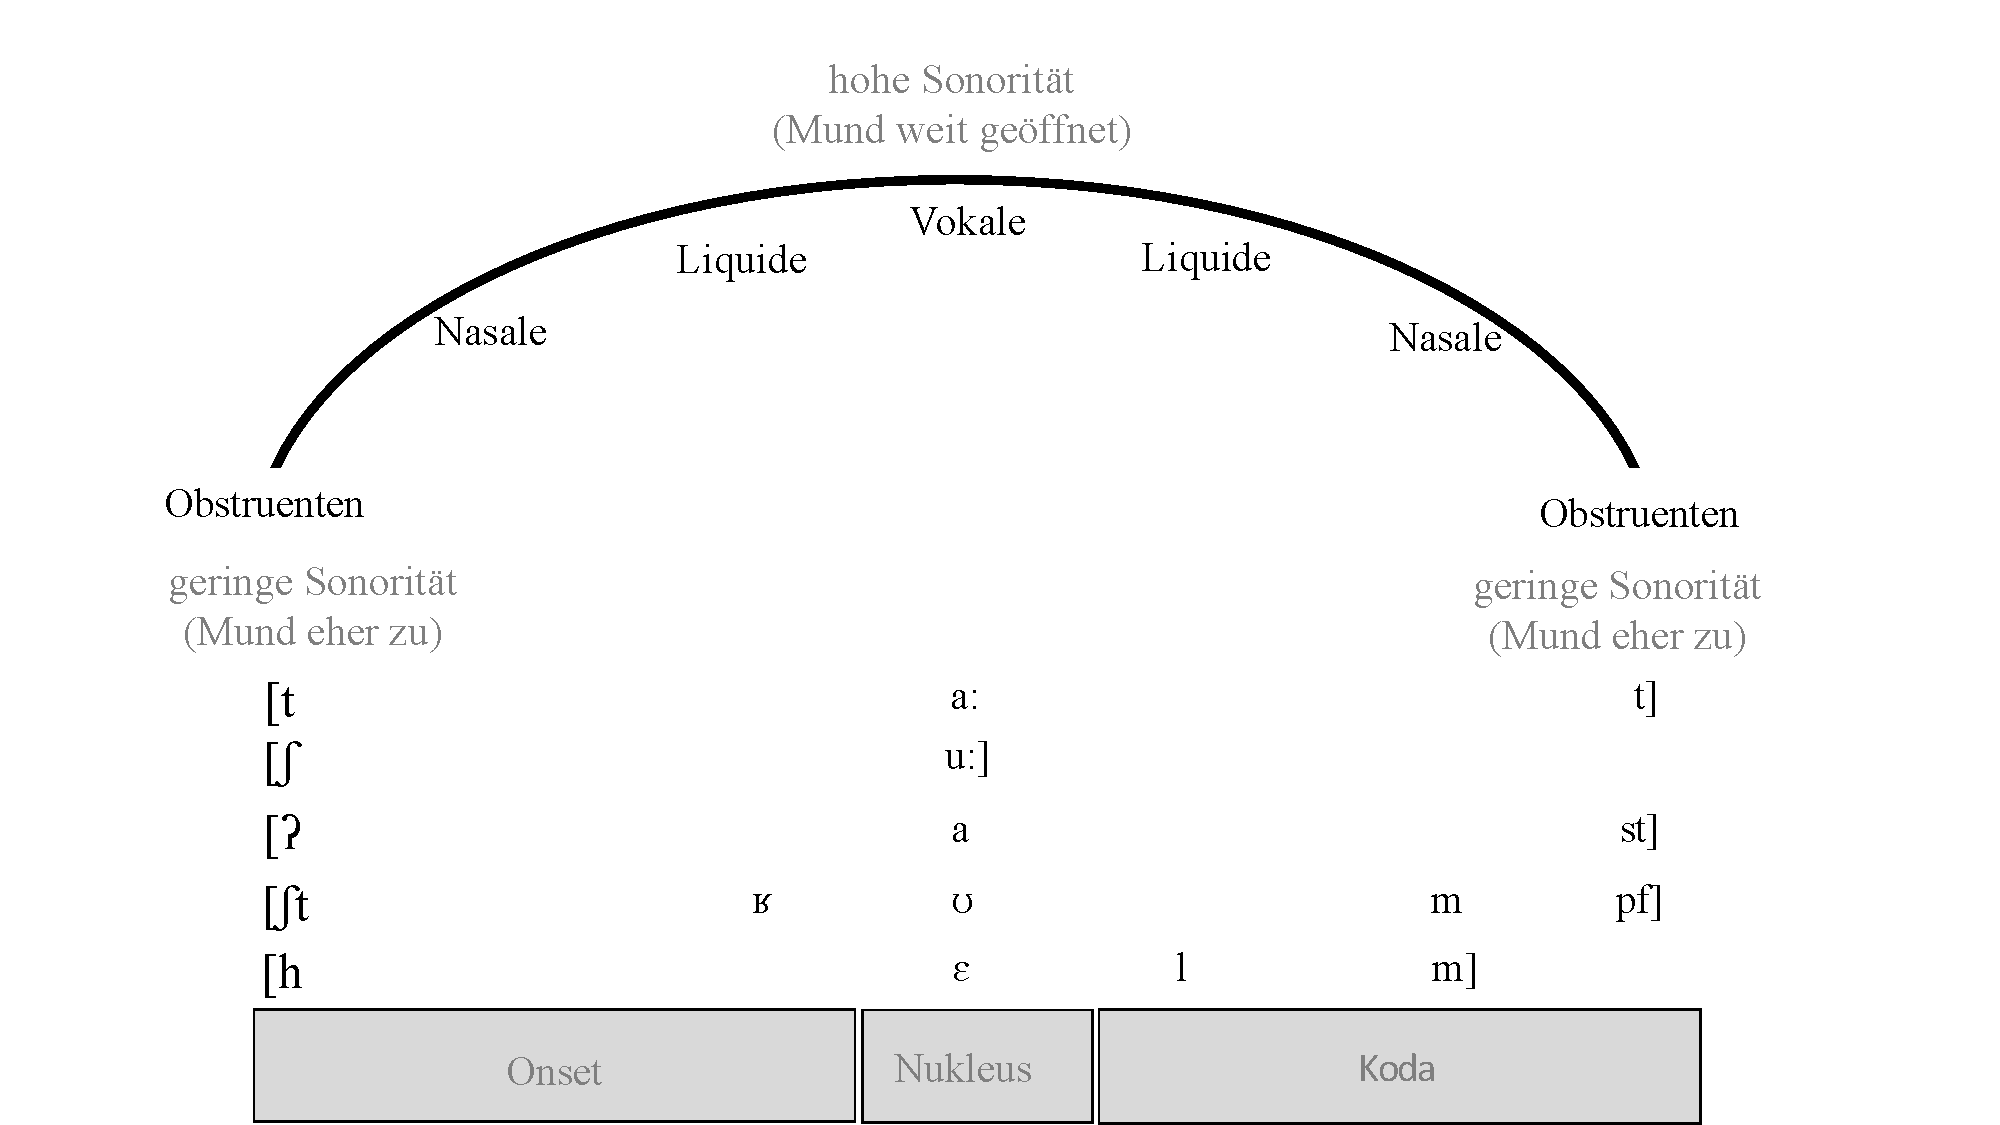
\includegraphics[width=1\textwidth]{figures/Sonoritaet.pdf}
    \caption{Sonoritätsverlauf in der Silbe nach \citet[224]{Hall2000}}
    \label{Abb:Sonoritaet}
\end{figure}




Das erste Beispiel, die Silbe \textit{Tat} \textipa{[ta:t]}, beginnt mit einem sehr wenig sonoren Laut, dem Obstruenten \textipa{[t]}, dem ein sehr sonorer Laut folgt, der Vokal \textipa{[a:]}. Am Ende steht wieder ein sehr wenig sonorer Laut, der Obstruent \textipa{[t]}. Wenn man die Laute vertauscht und eine Sequenz wie \textipa{[ata]} bildet, dann besteht diese Sequenz aus zwei Silben, denn die Sonorität fällt zunächst und steigt dann wieder an.

Das \is{Silbe!offen}zweite Beispiel in Abbildung~\ref{Abb:Sonoritaet}, \textit{Schuh} \textipa{[Su:]}, zeigt, dass Silben auch mit Vokal enden können. Die Schließbewegung des Mundes und der dadurch produzierte Abfall der Sonorität ist also optional. Solche Silben nennt man \textit{offene Silben}. Silben, bei denen dem Vokal noch ein Konsonant folgt, nennt man \is{Silbe!geschlossen}\textit{geschlossene Silben}.

Am dritten Beispiel, \textit{Ast} \textipa{[Past]}, kann man erkennen, dass betonte Silben im Deutschen jedoch nicht hochsonor beginnen können, also nicht mit einem Vokal. Vor dem Vokal muss mindestens ein Konsonant stehen. Sollte dies nicht der Fall sein, wird der Knacklaut als eine Art Dummy-Konsonant eingesetzt (vgl. Abschnitt~\ref{sec:Epenthese}). So entspricht auch eine Silbe wie \textit{Ast} \textipa{[Past]}  der Sonoritätshierarchie.

Das\is{Sonorant}\is{Obstruent} vierte Beispiel, \textit{Strumpf}, zeigt, dass nicht alle Konsonanten gleich sonor sind und die Konsonanten deshalb nicht in jeder beliebigen Reihenfolge auftreten können.\is{Nasal}\is{Lateral}\is{Vibrant}\is{Approximant} \textipa{[K]} und \textipa{[m]} sind als \is{Sonorant}Sonoranten\footnote{Sonoranten sind Nasale, Laterale, Vibranten und Approximanten (vgl. Abschnitt~\ref{sec:ObstSon}).}\footnote{Auch wenn \textipa{[K]} phonetisch gesehen ein Frikativ ist, zählt er innerhalb der Sonoritätsanalysen als Sonorant. Das liegt daran, dass das frikativische Allophon \textipa{[K]} nur eine Möglichkeit ist, den Konsonanten zu produzieren. Die vibrantischen Allophone \textipa{[r, \;R]} sind älter und hatten dadurch mehr Einfluss auf die Silbenstruktur der Wörter des Deutschen.} sonorer als die Obstruenten \textipa{[S, t, \t{pf}]}. Eine Sequenz wie \textipa{[KStU\t{pf}m]} ist keine mögliche Silbe, weil die sonoren Konsonanten \textipa{[K]} und \textipa{[m]} nicht weiter außen stehen können als die weniger sonoren Laute \textipa{[S, t, \t{pf}]}.

Innerhalb der Klasse der Sonoranten gibt es jedoch auch noch wesentliche Unterschiede in der Sonorität. So ist eine Silbe wie \textit{Helm} \textipa{[hElm]} (letztes Beispiel in Abbildung~\ref{Abb:Sonoritaet}) möglich, eine Sequenz wie \textipa{[hEml]} ist jedoch zweisilbig. Deshalb unterscheidet man innerhalb der Sonoranten noch zwischen den sogenannten \textit{Liquiden}\is{Liquid} (im Deutschen \textipa{/l/, /j/} und alle \textipa{/K/}-Allophone) und den Nasalen \textipa{/m, n, N/}. Die Liquide sind offener und stehen deshalb direkt um den Vokal herum. Die Nasale sind geschlossener und stehen zwischen den Obstruenten und den Liquiden.\footnote{Nasale werden, wie Plosive, mit einem totalen oralen Verschluss gebildet. Sie sind trotzdem sonorer als die Plosive, weil die Nasalpassage zum Vokaltrakt zählt, und diese Passage bei den Nasalen (im Unterschied zu den Plosiven) offen ist (vgl. Abschnitt~\ref{subsec:Nasale}).}

Eine \is{Onset}\is{Nukleus}\is{Koda}betonbare Silbe besteht also aus einem vokalischen Kern, um den sich Liquide, Nasale und Obstruenten wie die Häute einer Zwiebel positionieren.\footnote{Diese sehr einfache Klassifikation der Laute nach ihrer Sonorität ist für unsere Zwecke ausreichend. Eine feingliedrigere Einteilung findet man beispielsweise bei \citet[132]{RamersVater1991}, die Plosive als weniger sonor einstufen als Frikative, \textipa{[l]} als weniger sonor betrachten als \textipa{[K]} und zwischen hohen und tiefen Vokalen unterscheiden. \citet[72]{Wiese2011} folgt dem. \citet[61]{NoackPhonologie2016} übernimmt die Klassifikation von \citet{Jespersen1904}, der zusätzlich eine höhere So\-norität für stimmhafte Plosive und Frikative annimmt als für stimmlose. \textipa{[l]} und \textipa{[K]} werden als gleich sonor analysiert.} Den vokalischen Kern bezeichnet man, wie wir schon in Abschnitt~\ref{sec:KonsonantenundVokale} gesehen haben, als \textit{Nukleus}. Die Konsonanten die in der Silbe vor dem Nukleus stehen, nennt man den \textit{Onset} der Silbe. Alle Konsonanten, die dem Nukleus in der Silbe folgen, bilden die \textit{Koda} der Silbe. Silben können im Deutschen einen oder mehrere Konsonanten im Onset haben. Die Koda kann leer sein, sie kann aber auch mit einem oder mehreren Konsonanten besetzt sein. Die Konsonanten im Onset müssen so angeordnet sein, dass die Sonorität zum Nukleus hin ansteigt. Die Konsonanten in der Koda müssen so angeordnet sein, dass die Sonorität vom Nukleus her abfällt.

Mittels dieses Modells kann man nicht nur die Struktur von existierenden und möglichen Silben des Deutschen erklären, sondern auch die Lage von Silbengrenzen. Ein Wort wie \textit{Hamster} kann nicht als \textit{Ha-mster} silbifiziert werden, denn das \textipa{[m]} hat als Sonorant eine höhere Sonorität als der Frikativ \textipa{[s]} und kann deshalb nicht weiter vom Vokal der Silbe entfernt stehen als das \textipa{[s]}.


\subsection{Silbifizierung}\is{Silbifizierung}\label{subsec:Silbifizierung}

Für die Silbifizierung, also die Zuordnung von Lauten eines Wortes zu einzelnen Silben, gibt es unterschiedliche Gesetzmäßigkeiten. Diese Gesetzmäßigkeiten gehören zum impliziten Wissen von Sprecherinnen und Sprechern einer Sprache und erlauben es ihnen, weitgehend intuitiv zu silbifizieren. Der wichtigste Hinweis auf eine Silbengrenze kommt wie schon angedeutet über die Sonorität\is{Sonorität}: Silbengrenzen liegen im Deutschen in der Regel vor einem (lokalen) Sonoritätsminimum. 

Als Beispiel für diese Art der Lokalisierung der Silbengrenze sollen die Wörter \textit{Palme} und \textit{dreisilbig} betrachtet werden. Sprecherinnen und Sprecher des Deutschen silbifizieren diese Wörter \textit{Pal-me} und \textit{drei-sil-big}. In Abbildung~\ref{Abb:Silbifizierung} ist der Sonoritätsverlauf, den die Sprecherinnen und Sprecher akustisch wahrnehmen, als Kurve dargestellt. Die horizontale Achse zeigt die Abfolge der Laute, die vertikale Achse die Sonorität der einzelnen Laute.

Die erste Silbe von \textit{Palme} (oberer Teil der Abbildung), \textipa{[pal]}, besteht aus dem Obstruenten \textipa{[p]}, dem Vokal \textipa{[a]} und dem Sonoranten \textipa{[l]}. Die Sonorität steigt also von \textipa{[p]} zu \textipa{[a]} an und sinkt dann wieder für \textipa{[l]}. \textipa{[m]} hat eine geringere Sonorität als \textipa{[l]}. Da die Sonorität für das Schwa wieder ansteigt, ist \textipa{[m]} also das Sonoriätsminimum\is{Sonoritätsminimum} zwischen den beiden Vokalen. Die Silbengrenze\is{Silbengrenze} wird vor dieses Minimum gesetzt (gestrichelte Linie), deshalb silbifiziert man \textit{Pal-me} und nicht etwa \textit{Pa-lme} oder \textit{Palm-e}.\footnote{Die Silbifizierung \textit{Pal-me} schließt nicht aus, dass es Silben wie \textit{palm} geben könnte. Wenn ein Wort durch Derivation oder Flexion zweisilbig wird, kommt es häufig zu einer Verschiebung der Silbengrenze, um den Anforderungen bezüglich der Sonorität gerecht zu werden: \textit{Helm -- Hel-me, Wind -- win-dig}.}



\begin{figure}
    \centering
\begin{center}
	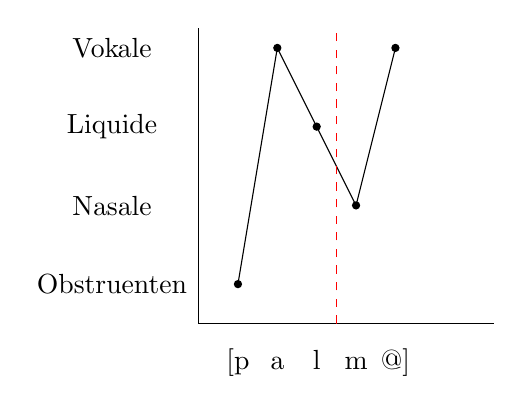
\begin{tikzpicture}[scale=0.5]
		\draw[black] (-1,0) -- (6.5,0) ; % x axis
		\draw[black] (-1,0) -- (-1,7.5); % y axis
		\node at (-3.2,1) {Obstruenten};
		\node at (-3.2,3) {Nasale};
		\node at (-3.2,5) {Liquide};
		\node at (-3.2,7) {Vokale};
		\draw[black] (0,1) -- (1,7) -- (2,5) -- (3,3) -- (4,7);
		\node at (0,-1) {\strut \textipa{[p}};
		\node at (1,-1) {\strut \textipa{a}};
		\node at (2,-1) {\strut \textipa{l}};
		\node at (3,-1) {\strut \textipa{m}};
		\node at (4,-1) {\strut \textipa{@}]};
		\fill (0,1) circle [radius=3pt];
		\fill (1,7) circle [radius=3pt];
		\fill (2,5) circle [radius=3pt];
		\fill (3,3) circle [radius=3pt];
		\fill (4,7) circle [radius=3pt];
        \draw[red, dashed] (2.5,0) -- (2.5,7.5);
	\end{tikzpicture}

    	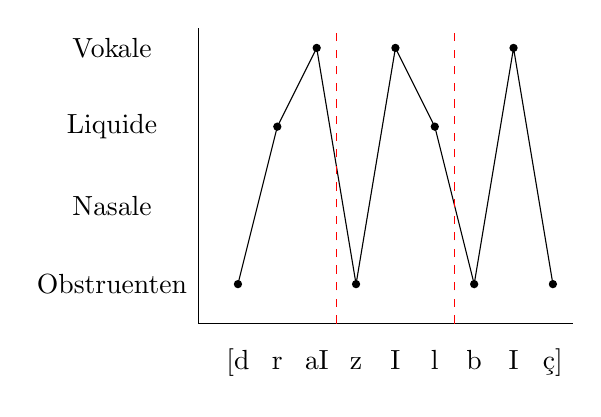
\begin{tikzpicture}[scale=0.5]
		\draw[black] (-1,0) -- (8.5,0) ; % x axis
		\draw[black] (-1,0) -- (-1,7.5); % y axis
		\node at (-3.2,1) {Obstruenten};
		\node at (-3.2,3) {Nasale};
		\node at (-3.2,5) {Liquide};
		\node at (-3.2,7) {Vokale};
		\draw[black] (0,1) -- (1,5) -- (2,7) -- (3,1) -- (4,7) -- (5,5) -- (6,1) -- (7,7) -- (8,1);
		\node at (0,-1) {\strut \textipa{[d}};
		\node at (1,-1) {\strut \textipa{r}};
		\node at (2,-1) {\strut \textipa{aI}};
		\node at (3,-1) {\strut \textipa{z}};
		\node at (4,-1) {\strut \textipa{I}};
		\node at (5,-1) {\strut \textipa{l}};
		\node at (6,-1) {\strut \textipa{b}};
        \node at (7,-1) {\strut \textipa{I}};
        \node at (8,-1) {\strut \textipa{\c{c}]}};
		\fill (0,1) circle [radius=3pt];
		\fill (1,5) circle [radius=3pt];
		\fill (2,7) circle [radius=3pt];
		\fill (3,1) circle [radius=3pt];
		\fill (4,7) circle [radius=3pt];
		\fill (5,5) circle [radius=3pt];
		\fill (6,1) circle [radius=3pt];
        \fill (7,7) circle [radius=3pt];
        \fill (8,1) circle [radius=3pt];
        \draw[red, dashed] (2.5,0) -- (2.5,7.5);% -- (5,6) -- (6,3);
        \draw[red, dashed] (5.5,0) -- (5.5,7.5);% -- (5,6) -- (6,3);
	\end{tikzpicture}
	
\end{center}
    
    \caption{Silbifizierung. Auf der vertikalen Achse ist die Sonorität der einzelnen Laute dargestellt. Die horizontale Achse zeigt die zeitliche Abfolge der Laute. Die gestrichelte Linien zeigt die Silbengrenze an.}
    \label{Abb:Silbifizierung}
\end{figure}

Bei dem Wort \textit{dreisilbig} (unterer Teil der Abbildung) beginnt die erste Silbe mit dem Obstruenten\is{Obstruent} \textipa{[d]}. Danach steigt die Sonorität an, zunächst zum zweiten Laut, dem Liquid \textipa{[K]}, und dann zum dritten, dem Vokal \textipa{[\t*{aI}]}. Danach fällt sie zum \textipa{[z]} hin ab, bevor sie zum \textipa{[I]} hin wieder ansteigt. Das \textipa{[z]} bildet also ein Minimum, sodass davor die erste Silbengrenze liegt. Vom \textipa{[I]} fällt die Sonorität über \textipa{[l]} zum \textipa{[b]} ab, bevor sie zum zweiten \textipa{[I]} wieder ansteigt. Das \textipa{[b]} bildet also wieder ein Sonoritätsminimum\is{Sonoritätsminimum}, sodass die zweite Silbengrenze\is{Silbengrenze} vor dem \textipa{[b]} liegt. 

Mittels der Sonorität\is{Sonorität} lassen sich viele, aber längst nicht alle Silbengrenzen begründen. Vor allem bei Konsonantenclustern\is{Konsonantencluster} ist die Sonorität als Erklärung für die Lage der Silbengrenzen nicht ausreichend. Als Beispiel dazu wird hier das Wort \textit{extrem} \textipa{[PEks\textprimstress tKe:m]} betrachtet. Laut Sonorität sollte man \textit{e-xtrem} \textipa{[PE\textprimstress kstKe:m]} silbifizieren,\is{Sonorität}\is{Silbifizierung} denn das Sonoritätsminimum ist bei \textipa{[k]} erreicht. Man silbifiziert jedoch \textit{ex-trem} \textipa{[PEks\textprimstress tKe:m]}.

Für\is{Phonotaktik}\is{Phonotaktik} die Abfolge von Lauten im Onset und in der Koda gibt es in jeder Sprache sogenannte \textit{phonotaktische Regeln} (vgl. Abschnitt~\ref{subsec:Phonotaktik}), die bestimmen, welche Laute in welcher Position und in welcher Kombination vorkommen können. Die phonotaktischen Regeln für das Deutsche schließen Sequenzen wie \textipa{[kstK]} im Onset einer Silbe aus, denn im Deutschen können maximal drei Konsonanten im Onset stehen \citep[68--69]{Hall1992}. Eine Silbe kann also nicht mit \textipa{[kstK]} beginnen. Auch \textipa{[stK]} ist vor dem Vokal im Standard nicht möglich. Zwar sind \textipa{/S/} und \textipa{/s/} (und nur diese beiden) als erste von drei Konsonanten im Onset möglich, das \textipa{/s/} verbindet sich dabei aber nur mit \textipa{/kK/} oder \textipa{/kl/} und selbst das nur in einigen Lehnwörtern (\textit{Skrupel, Sklave}). Die Silbengrenze bei \textit{extrem} wird also an der frühestmöglichen Position gesetzt, und die liegt nach dem \textipa{/s/}: \textipa{[PEks\textprimstress tKE:m]}.

Unabhängig davon sind Silbengrenzen durch den morphologischen Aufbau der Wörter beeinflusst \citep[72--73]{Bergmann2018}. Das Wort \textit{enteisen} beispielsweise wird \textit{ent-ei-sen} silbifiziert, obwohl die erste Silbengrenze laut Sonorität vor dem \textipa{/t/} stehen müsste (\textit{en-tei-sen}). Bei \textit{ent-} handelt es sich jedoch um ein \is{Präfix}Präfix. Präfixe verändern die Silbenstruktur der nachfolgenden Morpheme in der Regel nicht. Die Silbengrenze ist deshalb identisch mit der Morphemgrenze.

Eine Suffigierung\is{Suffigierung}\is{Suffix} hingegen kann zu einer Resilbifizierung führen \citep[73--74]{Bergmann2018}. Suffixe mit vokalischem Onset lösen eine Verschiebung der Silbengrenze nach links aus. So silbifiziert man \textit{Lö-sung} und nicht (nach Morphemen) \textit{Lös-ung}.

\subsection{Das Konstituentenstrukturmodell}\label{subsec:Silbenkonstituenten}\is{Konstituentenstrukturmodell}

In der Schriftsprachvermittlung wird inzwischen vielfach das sogenannte \textit{Häusermodell} (vgl. Exkurs~\ref{ex:SAM_Grundlage}, Seite~\pageref{ex:SAM_Grundlage}) genutzt, um Lernende mit der Struktur der Silbe vertraut zu machen und silbenspezifische Aussprache- und Orthografieregeln abzuleiten. In diesem Abschnitt geht es um das linguistische Modell, welches die Grundlage für das Häusermodell bildet.

\subsubsection{Onset, Nukleus und  Koda}

\is{Onset}\is{Nukleus}\is{Koda}Bei der Betrachtung der Sonorität wurde festgestellt, dass eine Silbe in der Regel aus einem vokalischen Kern besteht, der von Konsonanten umgeben ist. Den vokalischen Kern bezeichnet man als \textit{Nukleus}. Die Konsonanten vor dem Nukleus bilden den \textit{Onset}. Optional können dem Vokal noch Konsonanten folgen. Diese Konsonanten bilden die \textit{Koda} der Silbe. Man könnte eine Silbe also so darstellen wie in Abbildung~\ref{Abb:Silbenstruktur1}. Das σ (gesprochen \textit{Sigma}, griechisch für den Laut \textipa{[s]}) steht dabei für die Silbe, welche sich in Onset, Nukleus und Koda unterteilt. Eine solche Struktur nimmt für das Deutsche beispielsweise \citet[42--43]{Hall1992} an.

\begin{figure}
  \centering
  \begin{forest}
      [σ
        [Onset, ake
                  ]
          [Nukleus, ake
                    ]
          [Koda, ake
                    ]
      ]
  \end{forest}
  \caption{Eine mögliche Silbenstrukturanalyse nach \citet{Hall1992}}
    \label{Abb:Silbenstruktur1}
\end{figure}
\is{Onset}\is{Nukleus}\is{Koda}


\begin{Definition}{Onset, Nukleus und Koda}\label{def:OnsetNukleusKoda}

\noindent
Eine Silbe besteht aus Onset, Nukleus und Koda. Der Onset\is{Onset} einer Silbe besteht aus den Konsonanten, die vor dem Vokal stehen. Im Nukleus einer betonbaren Silbe steht ein vokalisches Segment. Die Koda besteht aus Konsonanten, die dem Vokal folgen.
\end{Definition}



\subsubsection{Reim}\label{subsec:Reim}\is{Reim}
\citet[134]{RamersVater1991} nehmen an, dass Nukleus und Koda enger miteinander verbunden sind als der Onset mit dem Nukleus. Wir folgen dem und werden deshalb ein etwas komplexeres Modell annehmen als das in Abbildung~\ref{Abb:Silbenstruktur1}, nämlich das Modell  in Abbildung~\ref{Abb:Silbenstruktur2} Bei diesem Modell werden Nukleus und Koda zunächst zu einem \textit{Reim} zusammengefasst. Erst in einem zweiten Schritt entsteht die Silbe aus Onset und Reim.
\is{Silbenstrukturanalyse}


\begin{figure}
  \centering
  \begin{forest}
      [σ, calign=last
        [Onset, ake
                  ]
        [Reim, calign=first
          [Nukleus, ake
                    ]
          [Koda, ake
                    ]
        ]
      ]
  \end{forest}
  \caption{Silbenstrukturanalyse mit Reim nach \citet{RamersVater1991}}
    \label{Abb:Silbenstruktur2}
\end{figure}

Für die Annahme des Reims gibt es unterschiedliche Argumente und Gegenargumente. Wir diskutieren hier drei davon, nämlich den Längenausgleich zwischen Nukleus und Koda, den poetischen Effekt von Reimen und Evidenz aus der Versprecherforschung. \citet[134--135]{RamersVater1991}\is{Längenausgleich} diskutieren den \textit{Längenausgleich} zwischen Nukleus und Koda, den man so formulieren kann: Wenn in einer Silbe viel Material im Nukleus ist, ist tendenziell wenig Material in der Koda. Wenn wenig Material im Nukleus ist, ist tendenziell mehr Material in der Koda. Tabelle~\ref{tab:Laengenausgleich} gibt einige Beispiele.

\begin{table}
\centering
\caption{Längenausgleich zwischen Nukleus und Koda. Die Zeilen entsprechen unterschiedlich komplexen Onsets (C=Konsonant), die Spalten unterschiedlich komplexen Kodas. Das jeweils erste Wort in jeder Zelle enthält einen Langvokal (LV), das zweite einen Kurzvokal (KV). \label{tab:Laengenausgleich}}
\begin{tabular}{lllllll}\lsptoprule
                &    \multicolumn{2}{c}{Koda leer}         &  \multicolumn{2}{c}{Koda C}         & \multicolumn{2}{c}{Koda CC} \\\midrule
      Onset          & LV & KV & LV & KV & LV & KV\\\midrule
C               & \textit{roh}& \textit{--}    & \textit{Moos} & \textit{Biss}     &  \textit{Mond} & \textit{Wunsch}\\ 
               & \textipa{[Ko:]} &     &  \textipa{[mo:s]} &  \textipa{[bIs]}      &  \textipa{[mo:nt]}&  \textipa{[vUnS]}\\
CC              & \textit{Floh} & \textit{--}  & \textit{Floß}& \textit{flott}  &  \textit{--} & \textit{blond} \\ 
              & \textipa{[flo:]}&  & \textipa{[flo:s]}& \textipa{[flOt]}     &   &  \textipa{[blOnt]}\\ 
CCC             & \textit{Stroh} & \textit{--} & \textit{Strom} & \textit{Stress}    &  \textit{--} & \textit{Strand} \\ 
             & \textipa{[StKo:]}&  & \textipa{[StKo:m]}& \textipa{[StKEs]}   &   & \textipa{[StKant]}\\ 
\lspbottomrule
\end{tabular}
\end{table}

Die Zeilen der Tabellen repräsentieren unterschiedlich komplexe Onsets. In der ersten Zeile stehen Wörter mit einem Onset, der aus einem Konsonanten (C) besteht: \textit{roh, Moos, Biss} usw. In der zweiten Zeile stehen Wörter mit zwei Konsonanten im Onset: \textit{Floh, Floß} usw. In der dritten Zeile stehen Wörter mit drei Konsonanten im Onset: \textit{Stroh, Strom} usw.

Die Spalten zeigen Unterschiede in der Komplexität der Koda: In der ersten Spalte stehen Wörter mit leerer Koda, \textit{roh} \textipa{[Ko:]}, \textit{Floh} \textipa{[flo:]} usw., in der zweiten Wörter mit nur einem Konsonanten in der Koda, \textit{Moos} \textipa{[mo:s]}, \textit{Floß} \textipa{[flo:s]} usw., in der dritten Wörter mit zwei Konsonanten in der Koda, \textit{Mond} \textipa{[mo:nt]}, \textit{Wunsch} \textipa{[wUnS]}. Wörter mit drei oder mehr Konsonanten in der Koda sind in der Regel flektierte Wörter (\textit{springst, brauchst} usw.). Diese Wörter ignorieren wir und betrachten nur Simplizia.\footnote{morphologisch einfache Wörter} Es gibt nur wenige Simplizia mit drei oder vier Konsonanten in der Koda, etwa \textit{Text} \textipa{[tEkst]}, \textit{Axt} \textipa{[Pakst]} oder \textit{selbst} \textipa{[zElpst]}.

Das erste Wort in jeder Zelle, markiert mit LV, enthält einen Langvokal (also viel Material im Nukleus), \zB \textit{roh, Floß}. In zwei Zellen fehlt dieses Wort (Onset CC und CCC, jeweils mit Koda CC), denn es gibt im deutschen Wortschatz kein passendes Wort. Wir werden gleich klären, warum. Das zweite Wort in jeder Zelle, markiert mit KV, enthält einen Kurzvokal im Nukleus (also wenig Material, \zB \textit{Biss, Strand}). In der ersten Spalte fehlen diese Wörter. 

Interessant sind vor allem diese Lücken in der Tabelle. Links in der Tabelle fehlen die Wörter mit Kurzvokal und rechts in der Tabelle fehlen die Wörter mit Langvokal. Es gibt keine Wörter -- allgemeiner: keine betonbaren Silben -- mit Kurzvokal und leerer Koda. \textipa{[KO]} oder \textipa{[StKO]} sind im Deutschen keine möglichen betonbaren Silben. Außerdem findet man nur sehr wenige Wörter mit Langvokalen und zwei oder mehr Konsonanten in der Koda, etwa \textit{Mond, wüst} und \textit{Obst}. 

Man kann also feststellen, dass es einen Längenausgleich\is{Längenausgleich} zwischen Nukleus und Koda gibt: Nach einem Kurzvokal im Nukleus muss die Koda besetzt sein. Nach einem Langvokal im Nukleus steht meist nur ein einziger Konsonant in der  Koda. 

Onset und Nukleus stehen nicht in einem solchen Ausgleichsverhältnis. Es gibt keine systematischen Lücken von Zeile zu Zeile. Wenn viel Material im Nukleus dazu führen würde, dass im Onset wenig stehen muss, sollte es Wörter wie \textit{Stroh} nicht geben. Es gibt aber zahlreiche Wörter mit komplexem Onset und Langvokal. Diese Beobachtungen sind im Einklang mit dem Modell in Abbildung~\ref{Abb:Silbenstruktur2}. Diesem Modell zufolge gibt es eine Abhängigkeit zwischen Nukleus und Koda. 

\citet[135--136]{RamersVater1991} führen als weiteres Argument für den Reim als Einheit -- und damit für das Modell in Abbildung~\ref{Abb:Silbenstruktur2} -- an, dass Reime (\textit{Maus -- Haus -- Laus}) poetische Effekte haben, die man bei Wörtern mit gleichem Onset und Nukleus nicht findet (\textit{Maus -- Maul -- Maut}).

Ein\is{Versprecher} weiteres Indiz dafür, dass Nukleus und Koda eine stärkere Verbindung eingehen als Onset und Nukleus, kommt aus der Versprecherforschung. Bei Versprechern, die durch Ersetzung von Segmenten entstehen, wird häufiger der Onset ausgetauscht als die Koda. Ein Beispiel aus \citet[321]{Schadeetal2008} ist (\ref{ex:jauter}). 
\ea
\ea [ ]{lauter Jubiläen}\label{ex:lauter}
\ex [*]{jauter Jubiläen}\label{ex:jauter}
\z
\z

Intendiert war die Äußerung \textit{lauter Jubiläen}, geäußert wurde aber \textit{jauter Jubiläen}. Während der Reim \textipa{[\t*{aU}]} unverändert bleibt, wird der eine Onset, \textipa{/l/}, durch den anderen, \textipa{/j/}, ersetzt.

Es gibt auch Versprecher, bei denen der gesamte Reim ausgetauscht wird, etwa in dem Versprecher von Jan Hofer aus der Tagesschau vom 24.06.2004, Beispiel (\ref{ex:genaunull2}). Hier wird offenbar der Reim \textipa{[\t*{aU}]} gegen den Reim \textipa{[Ul]} getauscht.
\ea
\ea [ ]{Es ist genau null Uhr.}\label{ex:genaunull1} 
\ex [*]{Es ist genull nau Uhr.}\label{ex:genaunull2}
\z 
\z

Versprecher, bei denen nur die Koda ausgetauscht wird (\textit{Es ist genaul nu Uhr.}) sind kaum denkbar. Gegen dieses Beispiel kann man einwenden, dass nicht der Reim, sondern die gesamte Silbe ausgetauscht wird.

Obwohl Argumente gegen das Modell in Abbildung~\ref{Abb:Silbenstruktur2} vorgebracht wurden, werden wir im Folgenden mit diesem Modell arbeiten. Grund dafür ist, dass zahlreiche Phänomene, vor allem die, die für die Graphematik relevant sind, mittels dieses Modells gut erklärbar sind.

\subsubsection{X-Positionen}
\is{X-Position}
Silben können sehr unterschiedlich komplex sein. In der Silbe \textit{rot} ist der Onset nur einfach besetzt, in der Silbe \textit{Stroh} dreifach. Um solche Unterschiede, aber auch um Aspekte wie den Längenausgleich im Reim darstellen zu können, folgen wir \citet[99]{Ramers1998} und \citet[239]{Hall2000} und erweitern das Modell der Silbe aus Abbildung~\ref{Abb:Silbenstruktur2} um eine sogenannte Skelettschicht\is{Skelettschicht}, die durch X-Positionen gekennzeichnet ist. Ein X steht dabei für eine abstrakte Zeiteinheit. Ein Kurzvokal entspricht einer einzigen X-Position, ein Langvokal oder Diphthong entspricht zwei X-Positionen. Konsonanten besetzen jeweils eine einzige X-Position.

Abbildung~\ref{fig:Konstmit} zeigt ein vollständiges \is{Konstituentenstrukturmodell}Konstituentenstrukturmodell für das einsilbige Wort \textit{mit}. Die Silbe untergliedert sich in Onset und Reim, der Reim unterteilt sich in Nukleus und Koda. In Onset, Nukleus und Koda befindet sich jeweils eine X-Position. Unter den X-Positionen ist das jeweilige Segment angegeben, welches die Position besetzt: Im Onset steht der Konsonant \textipa{[m]}, im Nukleus das kurze \textipa{[I]} und in der Koda das \textipa{[t]}. 

\begin{figure}
  \centering
  \begin{forest}
      [σ, calign=last
        [Onset, ake
          [X 
          [\textipa{m}]
          ]
        ]
        [Reim, calign=first
          [Nukleus, ake
            [X
            [\textipa{I}]
            ]
          ]
          [Koda, ake
          [X
          [\textipa{t}]
          ]
          ]
        ]
      ]
  \end{forest}
  \caption{Konstituentenanalyse der Silbe \textit{mit}}
  \label{fig:Konstmit}
\end{figure}

Die Struktur des einsilbigen Wortes \textit{rot} (vgl. Abbildung~\ref{fig:Konstrot}), ist ähnlich, aber im Nukleus stehen zwei X-Positionen, die durch das lange \textipa{[o:]} besetzt werden. 

\begin{figure}
  \centering
  \begin{forest}
      [σ, calign=last
        [Onset, ake
          [X 
          [\textipa{K}]
          ]
        ]
        [Reim, calign=first
          [Nukleus, ake
          [X, name=ERBaum]
    [X [\textipa{o:}]
    {\draw[-] (.north) -- (ERBaum.south);}
    ]
          ]
          [Koda, ake
          [X
          [\textipa{t}]
          ]
          ]
        ]
      ]
  \end{forest}
  \caption{Konstituentenanalyse der Silbe \textit{rot}}
  \label{fig:Konstrot}
\end{figure}

Mehrfach besetzte Onsets und Kodas sind ebenfalls darstellbar, etwa bei dem Einsilber \textit{Strumpf} (vgl. Abbildung~\ref{fig:Konststrumpf}). Hier ist der Onset mit drei X-Positionen besetzt. In der Koda stehen zwei X-Positionen. \is{Affrikate}Affrikaten sind ein einziges Segment, daher besetzt \textipa{[\t{pf}]} nur eine X-Position.


\begin{figure}
  \centering
  \begin{forest}
      [σ, calign=last
        [Onset, ake
          [X 
          [\textipa{S}]
          ]
          [X 
          [\textipa{t}]
          ]
          [X 
          [\textipa{K}]
          ]
        ]
        [Reim, calign=first
          [Nukleus, ake
            [X
            [\textipa{U}]
            ]
          ]
          [Koda, ake
          [X
          [m]
          ]
          [X
          [\textipa{\t{pf}}]
          ]
          ]
        ]
      ]
  \end{forest}
  \caption{Konstituentenanalyse der Silbe \textit{Strumpf}}
  \label{fig:Konststrumpf}
\end{figure}

Der Längenausgleich ist mit Hilfe dieses Modells wie folgt formulierbar: Wenn im Nukleus einer betonten Silbe nur eine X-Position besetzt ist, wie \zB bei \textit{mit} oder \textit{Strumpf}, muss die Koda mit mindestens einem X besetzt sein. Wenn im Nukleus zwei X-Positionen besetzt sind, wie bei \textit{rot}, kann die Koda leer sein.


\subsection{Phonotaktik}\label{subsec:Phonotaktik}\is{Phonotaktik}

Wie in Abschnitt~\ref{subsec:Sonoritaet} beschrieben, wird die Abfolge der Laute in der Silbe stark durch die Sonoritätshierarchie bestimmt. Beispielsweise gibt es im Deutschen Silben, die mit Plosiv+Liquid beginnen, etwa \textit{krank} oder \textit{Klang}, aber keine, die mit Liquid+Plosiv beginnen (*\textit{rkank}, *\textit{lkang}). 

Zusätzlich hat das Deutsche aber, wie jede andere Sprache auch, weitere Regeln, die den Silbenaufbau betreffen. Diese Regeln bezeichnet man als die \textit{Phonotaktik} der jeweiligen Sprache. Wir werden hier nur einige wenige Aspekte der deutschen Phonotaktik besprechen. Mehr über die Phonotaktik des Standarddeutschen findet man bei \citet{Hall1992} und \citet{Noske1993}.

Grundsätzlich folgen im \is{Onset}Onset Laute mit höherer Sonorität den Lauten mit geringerer \is{Sonorität}Sonorität. Außerdem lässt sich feststellen, dass bestimmte Laute gar nicht im Onset vorkommen. So gibt es keine Silben, deren Onset mit \textipa{/N/} besetzt ist\footnote{Es sei denn, der Konsonant fungiert als sogenanntes Silbengelenk (vgl. Abschnitt~\ref{subsec:Silbengelenk}), \zB in \textit{Enge}.} \citep[230]{Hall2000}. \textipa{/s/} kommt im Standarddeutschen ebenfalls nur eingeschränkt vor. Am Wortanfang kann es nicht allein einen Onset bilden, sondern nur mit anderen Konsonanten zusammen, wie beispielsweise \textipa{/sk/} in \textit{Skelett}. Einige Konsonanten können überhaupt nur alleine den Onset bilden, \zB \textipa{/\c{c}/}, wie in \textit{Chemie, Häuschen}, \textipa{/z/} wie in \textit{Sonne, Masern} und \textipa{/h/} wie in \textit{Haus, Uhu}, \citep[232]{Hall2000}. Silben wie \textit{*chla} \textipa{/\c{c}la/}, \textit{*sra} \textipa{/zra/} oder \textit{*hla} \textipa{/hla/} sind nicht möglich. Darüber hinaus sind eine Reihe von Kombinationen aus Obstruent und Sonorant im Onset nicht möglich, etwa \textipa{/km/, /tl/, /dv/} \citep[231]{Hall2000}.

Onsets mit drei X-Positionen haben noch stärkere Einschränkungen: Der erste der drei Konsonanten kann im nativen Wortschatz nur \textipa{/S/} sein: \textit{springen, Streit, Strauch} (vgl. Abbildung~\ref{fig:Konststrauch}).

\begin{figure}
  \centering
  \begin{forest}
      [σ, calign=last
        [Onset, ake
          [X 
          [\textipa{S}]
          ]
          [X 
          [\textipa{t}]
          ]
          [X 
          [\textipa{K}]
          ]
        ]
        [Reim, calign=first
           [Nukleus, ake
          [X, name=ERBaum]
    [X [\textipa{aU}]
    {\draw[-] (.north) -- (ERBaum.south);}
    ]
          ]
          [Koda, ake
          [X
          [\textipa{x}]
          ]
          ]
        ]
      ]
  \end{forest}
  \caption{Konstituentenanalyse der Silbe \textit{Strauch}. Bei einem dreigliedrigen Onset muss das erste Segment der postalveolare stimmlose Frikativ \textipa{[S]} sein.}
  \label{fig:Konststrauch}
\end{figure}

In der \is{Koda}Koda einer Silbe können in unflektierten Wörtern bis zu vier Konsonanten stehen, wie in \textit{selbst}. Flektierte Wörter können bis zu fünf Konsonanten in der Koda haben, wie der Genitiv der Substantivierung \textit{Selbst}, \textit{(ihres)} \textit{Selbsts}. Auch hier sind einige Konsonanten vollständig ausgeschlossen, etwa \textipa{/h/} und die stimmhaften Obstruenten. 


\begin{Exkurs}{Das Häusermodell nach Röber, Teil I}\label{ex:SAM_Grundlage}\is{Häusermodell}
\noindent 
Eine vereinfachte Form des Konstituentenstrukturmodells hat unter dem Namen \is{Häusermodell}\textit{Häusermodell} durch \citet{Roeber2013} Eingang in den Deutschunterricht gefunden. Dabei werden Silben als Häuser dargestellt, wie in den Abbildungen~\ref{fig:SAMHuetePhon} und \ref{fig:SAMHueftePhon} zu sehen ist. Betonte Silben werden durch ein Haus mit Dach symbolisiert und unbetonte durch ein Haus ohne Dach, \textit{Garage} genannt. Die Häuser haben je zwei sogenannte Zimmer. Dem Onset entspricht das Zimmer ganz links in jedem Haus. Der Reim wird als doppelt so großes zweites Zimmer mit einer durchbrochenen Wand dargestellt. 

\begin{figure}
    \centering
    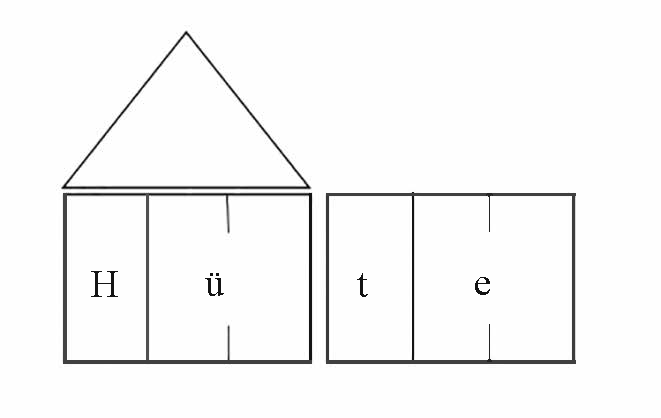
\includegraphics[width=0.5\textwidth]{figures/Huete.pdf}
    \caption{Darstellung der Silbenstruktur des Wortes \textit{Hüte} nach Röber. Die erste Silbe hat einen gespannten Vokal und ist offen.}
    \label{fig:SAMHuetePhon}
\end{figure}

\begin{figure}
    \centering
    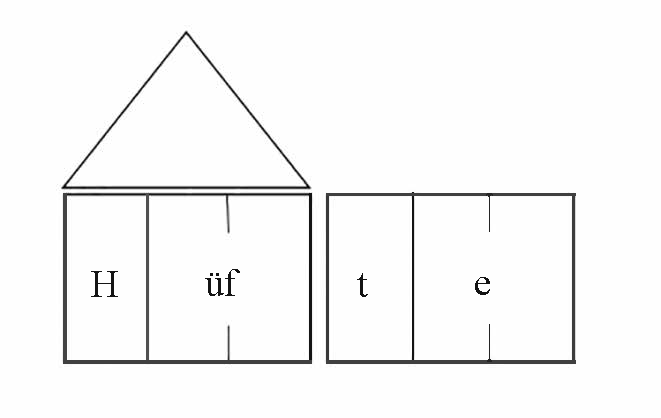
\includegraphics[width=0.5\textwidth]{figures/Huefte.pdf}
    \caption{Darstellung der Silbenstruktur des Wortes \textit{Hüfte} nach Röber. Die erste Silbe hat einen ungespannten Vokal und ist geschlossen.}
    \label{fig:SAMHueftePhon}
\end{figure}

In Abbildung~\ref{fig:SAMHuetePhon} ist das Wort \textit{Hüte} dargestellt. Dieses Wort besteht aus zwei Silben, einer betonten ersten und einer unbetonten zweiten Silbe. Das große Zimmer des Hauses mit Dach ist nur von einem Vokal bewohnt. Abbildung~\ref{fig:SAMHueftePhon} zeigt das Wort \textit{Hüfte}, bei welchem die Koda der ersten Silbe besetzt ist. Der Reim ist nun komplex: zwei Segmente bewohnen das Reim-Zimmer.

Das Häusermodell ist gut geeignet, um den \is{Längenausgleich}Längenausgleich im Reim der betonten Silbe darzustellen: Entweder ist das Reim-Zimmer von einem einzigen Vokal besetzt, dann wird dieser Vokal lang gesprochen (\textit{Hüte}). Oder das Reim-Zimmer ist von einem Vokal und einem Konsonanten bewohnt, dann wird der Vokal kurz gesprochen (\textit{Hüfte}).

Das Modell kann für unterschiedliche Zwecke genutzt werden. Am Anfang des Schriftspracherwerbs dient es dazu, die unterschiedliche Aussprache der Vokalgrapheme zu erklären (Langvokal vs. Kurzvokal). Wenn Lernende nur unter Zuhilfenahme der Phonem-Graphem-Korrespondenzen\footnote{vereinfacht: Zuordnung zwischen Lauten und Schriftzeichen (vgl. Abschnitt~\ref{sec:PGK})} lesen und die Silbenstruktur ignorieren, entstehen oft Produktionen wie \textipa{[\textprimstress hy:\textprimstress te:]} für \textit{Hüte} und \textipa{[\textprimstress hy:f\textprimstress te:]} für \textit{Hüfte} \citep[135]{Roeber2013}. Eine solche Leseaussprache erschwert oder verhindert sogar den lexikalischen Zugriff: Die Kinder erkennen das Wort gar nicht, welches sie gelesen haben, obwohl es ihnen bekannt ist. Besonders hinderlich ist diese Leseaussprache bei Wörtern auf \textit{-er} wie \textit{Winter}. Die Kinder lesen \textipa{[\textprimstress vi:n\textprimstress te:K]} und wissen nicht, was das Wort bedeuten soll.

Mittels des Häusermodells kann man drei Regeln vermitteln, die die Leseaussprache verbessern. Die erste betrifft die Aussprache des Vokals in der betonten Silbe. Ob dieser gespannt, wie in \textit{Hüte}, oder ungespannt, wie in \textit{Hüfte}, gesprochen wird, ist aufgrund des Längenausgleichs im Reim sehr oft aus der Silbenstruktur ableitbar: Wenn das Reim-Zimmer im Haus mit dem Dach ausschließlich einen Vokal enthält, wird der Vokal lang gesprochen. Wenn das Reim-Zimmer außer dem Vokal noch einen Konsonanten enthält, wird der Vokal kurz gesprochen.

Die zweite Regel betrifft die Aussprache der Vokale in der unbetonten Silbe. In unbetonten Silben können keine gespannten Vokale vorkommen. In der Garage gibt es also keine Langvokale. Meist wird der Vokal Schwa gesprochen.

Die dritte Regel betrifft das zu \textipa{[5]} vokalisierte r. Vokalisierte r-Laute treten im Reim einer Silbe auf, wie bei \textit{Winter, wir, Tor}. Ein orthografisches <r> im Reim-Zimmer wird also als tiefes Schwa gesprochen, während ein r im linken Zimmer als \textipa{[K, r]} oder \textipa{[\;R]}  gesprochen wird.

Das Häusermodell hat zahlreiche andere Anwendungsmöglichkeiten, etwa für die Platzierung des Dehnungs-\textit{h}, für die Konsonantenverdopplung beim Silbengelenk und für die Fremdwortschreibung (\cite{Bredel2011} und \cite{Roeber2013}, vgl. Exkurs~\ref{Exkurs:SAM}).


\end{Exkurs}

\subsection{Silbenpräferenzgesetze}\label{subsec:Silbenpräferenz}\is{Silbenpräferenzgesetz}

Beim Spracherwerb kann man beobachten, dass bestimmte Silben sehr früh erworben werden und andere später. Ab einem Alter von 6 Monaten produzieren Kinder sogenannte CV-Silben\is{Silbe!CV} \citep[23]{Falk2008}. Das sind Silben, die aus einem Konsonanten und einem Vokal bestehen, etwa \textipa{[ba]}. Erst mit 10 Monaten kommen CVC-Silben\is{Silbe!CVC} wie \textipa{[bab]} dazu. Auch die ersten Wörter wie \textit{Mama} und \textit{Papa} bestehen aus CV-Silben. Wenn man die Sprachen der Welt betrachtet, kann man feststellen, dass die CV-Silbe in allen Sprachen existiert \citep[213]{Hall2000}, während komplexere Silben wie beispielsweise CCCVCC bei \textit{Strumpf} in vielen Sprachen nicht möglich sind.

Es scheint intuitiv nachvollziehbar, dass Kinder zunächst einfachen Silben wie CV den Vorzug vor komplexeren wie CCCVCC geben.\is{Silbe!VC} Aber warum beginnen sie nicht \zB mit VC-Silben wie \textipa{[ab]}, welche ja genauso einfach sind? Das liegt daran, dass die CV-Silbe einen Sonoritätsverlauf hat, der es sehr einfach macht, die Silbengrenze zu erkennen. Bei einem Wort, das aus CV-Silben besteht, wie \zB \textit{Papa}, steigt die Sonorität in der ersten Silbe vom Onset zum Nukleus hin an. Die zweite Silbe beginnt wieder mit einer niedrigeren Sonorität, sodass dort ein Sonoritätsminimum liegt und die Silbengrenze vor diesem Minimum verortet werden kann.

Ein Wort aus VC-Silben wie \textipa{[am.am]} könnte man anhand der Sonorität allein nicht korrekt silbifizieren. Im Deutschen behilft man sich bei betonten Silben damit, an der Stelle der Silbengrenze einen Knacklaut einzusetzen: \textipa{[Pam.Pam]}.\footnote{Eine Alternative zu \textipa{[Pam.Pam]} wäre \textipa{[Pa\.*mam]} mit dem ersten \textipa{/m/} als Silbengelenk. Damit wäre der Onset der zweiten Silbe jedoch ebenfalls besetzt (vgl. Abschnitt~\ref{subsec:Silbengelenk}).} Der Knacklaut ist ein Obstruent und damit ein niedrigsonoriger Laut. Dadurch wird die Silbengrenze prominent markiert.

Diese in den Sprachen der Welt zu findenden Vorlieben für bestimmte Silben beschreiben \citet[212--217]{Hall2000} und \citet[229--230]{Pompino-Marschall2020} als Silbenpräferenzgesetze.
Man unterscheidet das \textit{Silbenanlautgesetz}, das \textit{Silbenkerngesetz} und das \textit{Silbenauslautgesetz}. 

Laut \is{Silbenpräferenzgesetz!Silbenanlautgesetz}Silbenanlautgesetz haben (in den Sprachen der Welt und im Spracherwerb) präferierte Silben möglichst nur einen Laut im Onset, der möglichst wenig sonor ist. Ein Onset wie \textipa{/p/} ist demnach besser als \textipa{/l/} oder \textipa{/kl/}.

Das \is{Silbenpräferenzgesetz!Silbenkerngesetz}Silbenkerngesetz besagt, dass im Silbenkern Laute mit hoher Sonorität präferiert werden. Ein vokalischer Kern ist also besser als ein sonorantischer, wie er etwa in der zweiten Silbe von \textit{Mantel} nach der Tilgung des Schwa auftritt (vgl. Abschnitt \ref{sec:Schwatilgung}): \textipa{[\textprimstress man.t\s{l}]}.

Laut \is{Silbenpräferenzgesetz!Silbenauslautgesetz}Silbenauslautgesetz sollten in der Koda möglichst wenige Laute stehen, die möglichst sonor sein sollten. Außerdem sollte die Sonorität vom Silbenkern aus abfallen. Eine Silbe mit leerer Koda ist demnach die mit der höchsten Präferenz.


Im Spracherwerb kann man die Wirkung der Silbenpräferenzgesetze gut beobachten. In einem bestimmten Alter vereinfachen Kinder die weniger präferierten CVC-Silben wie bei \textit{Mehl} zu den präferierteren CV-Silben wie \textipa{[me:]} \citep[25]{Falk2008}. Silben mit komplexem Onset wie \textit{krank} \textipa{[\textprimstress kKaNk]} werden zu Silben mit einfachem Onset modifiziert. Dabei wird den wenig sonoren Lauten der Vorzug gegeben. So wird  \textipa{[\textprimstress kKaNk]} zu \textipa{[\textprimstress kaNk]} statt \textipa{[\textprimstress KaNk]} vereinfacht \citep[58]{Muelleretal2018}. Der Onset \textipa{/k/} entspricht dem Silbenanlautgesetz: Er besteht aus einem einzigen, wenig sonoren Laut.

Silbenpräferenzgesetze gelten niemals absolut. Wenn wir aus dem Silbenanlautgesetz ableiten, dass Onsets besetzt sein sollen, dann bedeutet das nicht, dass es keine Silben mit unbesetztem Onset gibt. Es bedeutet lediglich, dass, wenn die Bedingungen das hergeben, der Onset besetzt wird. Für das Standarddeutsche kann man sagen, dass die Silbenpräferenzgesetze dazu führen, dass Onsets betonter Silben immer besetzt sind. Aus dem Silbenkerngesetz kann man ableiten, dass der Silbenkern einer betonten Silbe mit mindestens zwei X-Positionen besetzt sein muss.

\subsection{Silbengelenke}\label{subsec:Silbengelenk}\is{Silbengelenk}

Wie im Abschnitt~\ref{subsec:Sonoritaet} angemerkt, verfügen viele Kinder schon im Vorschulalter über die Kompetenz, Wörter wie \textit{Kinder} oder \textit{Tage} in Silben zu zerlegen. Eine Ausnahme bilden Wörter wie \textit{Messer} oder \textit{Löffel}. Erwachsene sind bei solchen Wörtern mit \is{Doppelkonsonanz}Doppelkonsonanz durch ihre Orthografieerfahrung geneigt zu glauben, die Silbifizierung sei \textit{Mes-ser} und \textit{Löf-fel}. Das würde aber voraussetzen, dass man das \textipa{/s/} bzw. das \textipa{/f/} doppelt spricht. Davon, dass das nicht der Fall ist, kann man sich überzeugen, wenn man Wörter mit Plosiv an der fraglichen Stelle betrachtet, etwa \textit{Hütte}. Wenn man zwei Plosive sprechen würde, müsste man zwei Verschlusslösungen produzieren, wie beim Stottern. 

\citet{Risel2000} zeigt, dass Kinder bei der Silbifizierung dieser Wörter völlig anders vorgehen. Für Zweitklässler zeigt er, dass etwa 60\% der Kinder die Silbengrenze hinter den Vokal setzen: \textit{Me-sser, Lö-ffel}. Etwa 30\% nutzen eine sogenannte Gelenkartikulation mit gedehntem \textipa{/s/} bzw. 
\textipa{/f/} zwischen den Silben: \textipa{[\textprimstress mEs::5]}. Und etwa 10\% setzen die Silbengrenze hinter den fraglichen Konsonanten: \textit{Mess-er, Löff-el}. Erst in der dritten Klasse gibt es zunehmend orthografische Gliederungen nach dem Muster \textit{Mes-ser} und \textit{Löf-fel}.

Warum sind die Antworten der Kinder hier so vielfältig, obwohl sie bei Wörtern ohne Doppelkonsonanz relativ einheitlich sind? Das liegt daran, dass bei Wörtern wie \textit{Messer} und \textit{Löffel} ein \textit{Silbengelenk}\is{Silbengelenk} vorliegt: Ein Konsonant gehört nicht klar zu der einen oder anderen Silbe, sondern er steht zwischen den Silben. Während die \citet[862]{Duden2016} vom Silbengelenk spricht, benutzt \citet[35--36]{Wiese2000} den Terminus \textit{ambisilbischer Konsonant}\is{ambisilbischer Konsonant}. Die neue \citet[862]{Duden2022} verwendet beide Begriffe. Bei einem Wort wie \textit{Messer} steht das \textipa{/s/} also sowohl in der Koda der ersten Silbe als auch im Onset der zweiten. In der Transkription werden ambisilbische Konsonanten durch einen Punkt\is{Silbengrenze} unter dem Konsonanten markiert: \textipa{[\textprimstress mE\.*s5]}.

Wie kommt es dazu, dass ein Konsonant einen solchen Status hat? Um diese Frage zu beantworten schauen wir uns zunächt noch einmal an, welche Bedingungen erfüllt sein müssen, damit eine Silbe betonbar ist (vgl Abschnitt~\ref{subsec:Betonbarkeit}). Eine betonbare Silbe muss eine gewisse Mindestmenge an Material im Reim aufweisen. Entweder muss im Nukleus ein Langvokal stehen, oder ein Diphthong, oder der Nukleus ist mit einem Kurzvokal besetzt, dann darf die Koda aber nicht leer sein. In Abschnitt~\ref{subsec:Reim} hatten wir das formuliert als: Im Reim einer betonten Silbe müssen mindestens zwei X-Positionen besetzt sein. Bei einer Silbe wie \textit{See} stehen diese beiden X-Positionen im Nukleus (vgl. Abbildung~\ref{fig:KonstSee}), bei der Silbe \textit{Bett} steht eine im Nukleus und eine in der Koda, (vgl. Abbildung~\ref{fig:KonstBett}). Bei \textit{Messer} besetzt der Kurzvokal \textipa{/E/} im Nukleus nur eine X-Position. Da die erste Silbe aber betont ist, muss eine weitere X-Position im Reim besetzt sein. Das leistet das \textipa{/s/} in der Koda. 

\begin{figure}
  \centering
  \begin{forest}
      [σ, calign=last
        [Onset, ake
          [X 
          [\textipa{z}]
          ]
        ]
        [Reim, calign=first
          [Nukleus, ake
          [X, name=ERBaum]
    [X [\textipa{e:}]
    {\draw[-] (.north) -- (ERBaum.south);}
    ]
          ]
          [Koda, ake
          ]
        ]
      ]
  \end{forest}
  \caption{Konstituentenanalyse der Silbe \textit{See}. Im Nukleus dieser betonbaren Silbe sind zwei X-Positionen besetzt.}
  \label{fig:KonstSee}
\end{figure}

\begin{figure}
  \centering
 \begin{forest}
      [σ, calign=last
        [Onset, ake
         [X 
          [\textipa{b}]
          ]
        ]
        [Reim, calign=first
          [Nukleus, ake
              [X [\textipa{E}]
            ]
          ]
          [Koda, ake
              [X [\textipa{t}]]
          ]
        ]
      ]
  \end{forest}
  \caption{Konstituentenanalyse der Silbe \textit{Bett}. Im Reim dieser betonbaren Silbe sind zwei X-Positionen besetzt, eine im Nukleus und eine in der Koda.}
  \label{fig:KonstBett}
\end{figure}


\begin{figure}[!htbp]
  \centering
  \begin{forest}
  [Wort
      [σ, calign=last
        [Onset, ake
          [X
          [\textipa{m}]
          ]
        ]
        [Reim, calign=first
          [Nukleus, ake
            [X
            [\textipa{E}]
            ]
          ]
          [Koda, ake, name=ERBaum]
        ]
      ]
      [σ, calign=last
        [Onset, ake
          [X
          [\textipa{\.*s}]
          ]
          {\draw[-] (.north) -- (ERBaum.south);}
        ]
        [Reim
          [Nukleus, ake
            [X
            [\textipa{5}]
            ]
          ]
          [Koda, ake
          ]
        ]
      ]
     ]
  \end{forest}
  \caption{Konstituentenanalyse von \textit{Messer}. \textipa{[s]} ist ein Silbengelenk. Es besetzt gleichzeitig die Koda der ersten Silbe, sodass diese Silbe betonbar wird, und den Onset der zweiten.}
  \label{fig:KonstMesser}
\end{figure}

Nach dem Silbenanlautgesetz ist eine Silbe präferierter, wenn der Onset besetzt ist. Das \textipa{/s/} von \textit{Messer} wird also nicht nur in der Koda der ersten Silbe benötigt, sondern auch, um den Onset der zweiten Silbe zu besetzen (vgl. Abbildung~\ref{fig:KonstMesser}). 

Um die Abgrenzung zwischen ambisilbischen Konsonanten und anderen Konsonanten besser zu verstehen, werden im Folgenden die Wörter \textit{Taste} \textipa{[\textprimstress tas.t@]} (vgl. Abbildung~\ref{fig:KonstTaste}) und \textit{Tasse} \textipa{[\textprimstress ta\.*s@]} (vgl. Abbildung~\ref{fig:KonstTasse2}) verglichen. Bei \textit{Taste} besteht die erste Silbe aus drei Lauten: \textipa{[tas]}. Der erste Konsonant steht im Onset, der Vokal steht im Nukleus und der zweite Konsonant steht in der Koda. Die Silbe ist betonbar, denn zwei X-Positionen im Reim sind besetzt, eine davon im Nukleus, die andere in der Koda. In der zweiten Silbe \textipa{[t@]} steht der Konsonant im Onset und der Vokal im Nukleus. Der Onset ist also besetzt, die Silbe ist eine laut Silbenanlautgesetz präferierte Silbe. Zwar ist im Reim nur eine X-Position besetzt, aber das ist kein Problem, da die Silbe ja nicht betont werden soll.




\begin{figure}[!htbp]
  \centering
  \begin{forest}
  [Wort
      [σ, calign=last
        [Onset, ake
          [X
          [\textipa{t}]
          ]
        ]
        [Reim, calign=first
          [Nukleus, ake
            [X
            [\textipa{a}]
            ]
          ]
          [Koda, ake,
            [X
            [\textipa{s}]
            ]
          ]
        ]
      ]
      [σ, calign=last
        [Onset, ake
          [X
          [\textipa{t}]
          ]
        ]
        [Reim
          [Nukleus, ake
            [X
            [\textipa{@}]
            ]
          ]
          [Koda, ake
          ]
        ]
      ]
     ]
  \end{forest}
  \caption{Konstituentenanalyse von \textit{Taste}. \textipa{[s]} steht in der Koda der ersten Silbe. Es ist kein Silbengelenk, denn der Onset der zweiten Silbe ist durch \textipa{[t]} besetzt.}
  \label{fig:KonstTaste}
\end{figure}

Bei \textit{Tasse} steht das \textipa{[t]} im Onset der ersten Silbe und das \textipa{[a]} im Nukleus (vgl. Abbildung \ref{fig:KonstTasse2}). Überspringen wir für den Moment das \textipa{[s]} und schauen uns die zweite Silbe an. Dort steht noch ein Vokal im Nukleus. Das \textipa{[s]} muss nun zwei Funktionen gleichzeitig erfüllen: Erstens muss eine zweite X-Position im Reim der ersten Silbe besetzt werden, damit die Silbe betonbar wird. Zweitens soll dem Silbenanlautgesetz zufolge nach Möglichkeit der Onset der zweiten Silbe besetzt werden. Für diese beiden Aufgaben gibt es aber nur einen Konsonanten, das \textipa{[s]}. Dieser Konsonant wird also an beiden Stellen gebraucht und wird deshalb zum ambisilbischen Konsonanten. 

\begin{figure}[H]
  \centering
  \begin{forest}
  [Wort
      [σ, calign=last
        [Onset, ake
          [X
          [\textipa{t}]
          ]
        ]
        [Reim, calign=first
          [Nukleus, ake
            [X
            [\textipa{a}]
            ]
          ]
          [Koda, ake, name=ERBaum]
        ]
      ]
      [σ, calign=last
        [Onset, ake
          [X
          [\textipa{\.*s}]
          ]
          {\draw[-] (.north) -- (ERBaum.south);}
        ]
        [Reim
          [Nukleus, ake
            [X
            [\textipa{@}]
            ]
          ]
          [Koda, ake
          ]
        ]
      ]
     ]
  \end{forest}
  \caption{Konstituentenanalyse von \textit{Tasse}. \textipa{[s]} ist ein Silbengelenk. Es besetzt gleichzeitig die Koda der ersten Silbe und den Onset der zweiten.}
  \label{fig:KonstTasse2}
\end{figure}

Ein Silbengelenk kann man als eine Art Notlösung ansehen, wenn nur ein Konsonant vorhanden ist, der aber an zwei Stellen gebraucht wird. Ein Silbengelenk tritt also immer dann auf, wenn drei Bedingungen zusammenfallen:
\begin{itemize}
    \item Eine betonte Silbe geht einer unbetonten voraus.
    \item In der betonten Silbe steht ein Kurzvokal.
    \item Zwischen den beiden vokalischen Kernen steht nur ein Konsonant.
\end{itemize}

Man kann sagen, dass ein Silbengelenk leere Onsets\is{Onset} verhindert. Das bedeutet aber nicht, dass es gar keine leeren Onsets mehr gibt. Wenn zwischen zwei vokalischen Kernen kein Konsonant steht, dann ist der Onset der zweiten Silbe leer, etwa in den Wörtern \textit{Bauer} \textipa{[\textprimstress baU.5]}, \textit{Ehe} \textipa{[\textprimstress Pe:.@]}, \textit{Bio} \textipa{[\textprimstress bi:.o]}. Orthografisch wird der leere Onset in den meisten Fällen durch ein \is{silbentrennendes h}silbentrennendes h gefüllt: \textit{sehen, Mühe, leihen} (vgl. Abschnitt~\ref{AbschnittDehnungsh}). Dieses h wird im Standard aber nicht gesprochen.\footnote{Schon \citet{Levitt1978} stellte jedoch fest, dass Sprecherinnen und Sprecher mit der zunehmenden Alphabetisierung dazu neigen, ihre Aussprache an die Schrift anzupassen. In bestimmten Kontexten, zum Beispiel beim Diktieren, neigen Sprecherinnen und Sprecher deshalb dazu, das silbentrennende h doch mitzusprechen. Auch sind alphabetisierte Personen der Meinung, dass silbentrennende h hören zu können. Im Standard ist es jedoch nicht vorgesehen.} Wenn die Schreibung kein h aufweist, setzen Leseanfänger nicht selten einen Knacklaut als Ersatz ein: \textipa{[\textprimstress bi:.Po]}, was die Worterkennung -- den lexikalischen Zugriff -- erschwert.

Orthografisch werden Silbengelenke oft durch Doppelkonsonanz gekennzeichnet: \textit{Keller, Sonne, Bretter} (vgl. Abschnitt~\ref{sec:Silbengelenksschreibungen}). Aber nicht jede \is{Doppelkonsonanz}Doppelkonsonanz zeigt ein \is{Silbengelenk}Silbengelenk an. Wenn ein Wort aufgrund eines Silbengelenks mit Doppelkonsonanz geschrieben wird, werden alle anderen Wörter der Wortfamilie auch mit Doppelkonsonanz geschrieben, selbst wenn sie kein Silbengelenk haben. So schreibt man \textit{Brett} und \textit{Brettchen} mit <tt>, weil das Silbengelenk in \textit{Bretter} durch <tt> gekennzeichnet wird -- und das, obwohl es weder in \textit{Brett} noch in \textit{Brettchen} ein Silbengelenk gibt.

Auch der umgekehrte Schluss, dass ein Wort ohne Doppelkonsonanz garantiert kein Silbengelenk hat, ist falsch. Komplexe Grapheme\is{Graphem!komplex} wie beispielsweise <sch> und <ch> werden als Silbengelenk nicht verdoppelt: \textit{wischen, machen}. Das Wort \textit{Tasche} beispielsweise ist von der Silbenstruktur her identisch mit \textit{Tasse}, denn das \textipa{/S/} bildet ein Silbengelenk. Trotzdem enthält \textit{Tasche} keine Doppelkonsonanz.

Eine \is{Doppelkonsonanz}Doppelkonsonanz folgt immer einem ungespannten Vokal. Man kann aus einer Doppelkonsonanz deshalb schlussfolgern, dass der vorangehende Vokal ungespannt zu lesen ist. Umgekehrt kann man \textit{nicht} schlussfolgern, dass alle ungespannten Vokale durch Doppelkonsonanz zu kennzeichnen sind, denn sonst müssten Wörter wie \textit{Wald, Ende, Wirt} <Walld, Ennde, Wirrt> geschrieben werden. 

\subsection{Beispielanalysen}

Um eine Konstituentenstrukturanalyse zu erstellen, geht man am besten wie folgt vor: Man transkribiert das zu analysierende Wort und gliedert es in Silben, sucht in jeder Silbe den vokalischen Nukleus und ordnet die Konsonanten vor dem Nukleus dem Onset zu und die Konsonanten, die dem Nukleus innerhalb der Silbe folgen, der Koda. 

Als erstes Beispiel betrachten wir das Wort \textit{streichen}. Zunächst transkribieren wir: \textipa{[\textprimstress StK\t*{aI}.\c{c}@n]}. Eine alternative Transkription mit Schwa-Tilgung wäre \textipa{[\textprimstress StK\t*{aI}.\c{c}\s{n}]}. Wir analysieren zunächst die erste Variante. Die erste Silbe endet nach dem Diphthong. Der Diphthong ist der Nukleus. Alles, was davor steht \newline-- nämlich \textipa{[StK]} -- steht im Onset. Dem Nukleus folgt kein weiterer Konsonant in der ersten Silbe, also ist die Koda leer. In der zweiten Silbe \textipa{[\c{c}@n]} bildet der Schwa-Laut den vokalischen Kern, der Konsonant vor dem Schwa, \textipa{[\c{c}]} steht im Onset, der Konsonant, der dem Schwa folgt, \textipa{[n]}, steht in der Koda. Jedem Konsonanten wird ein X zugeordnet. Dem Diphthong werden zwei X-Positionen zugeordnet, dem Schwa-Laut nur eine. Es ergibt sich die Analyse in Abbildung~\ref{fig:Bspstreichen1}.

\begin{figure}[!htbp]
  \centering
  \begin{forest}
  [Wort
      [σ, calign=last
        [Onset, ake
          [X
          [\textipa{S}]
          ]
          [X
          [\textipa{t}]
          ]
          [X
          [\textipa{K}]
          ]
        ]
        [Reim, calign=first
          [Nukleus, ake
          [X, name=ERBaum]
    [X [\textipa{\t*{aI}}]
    {\draw[-] (.north) -- (ERBaum.south);}
    ]
          ]          
          [Koda, ake,
          ]
        ]
      ]
      [σ, calign=last
        [Onset, ake
          [X
          [\textipa{\c{c}}]
          ]
        ]
        [Reim
          [Nukleus, ake
            [X
            [\textipa{@}]
            ]
          ]
          [Koda, ake
            [X
            [\textipa{n}]
            ]
          ]
        ]
      ]
     ]
  \end{forest}
  \caption{Konstituentenanalyse von \textit{streichen} }
  \label{fig:Bspstreichen1}
\end{figure}

Um eine Konstituentenstrukturanalyse für die zweite Variante \textipa{[\textprimstress StK\t*{aI}.\c{c}\s{n}]} zu erstellen, teilen wir das Wort wieder in Silben ein. Die erste Silbe wird wie in Abbildung~\ref{fig:Bspstreichen1} analysiert. In der zweiten Silbe fehlt der vokalische Kern. Dass wir das Wort trotzdem als zweisilbig wahrnehmen, liegt daran, dass der sonore Laut \textipa{[n]} die Funktion des Vokals übernimmt. \textipa{[n]} erscheint deshalb im Nukleus, siehe Abbildung~\ref{fig:Bspstreichen2}.

\begin{figure}[!htbp]
  \centering
  \begin{forest}
  [Wort
      [σ, calign=last
        [Onset, ake
          [X
          [\textipa{S}]
          ]
          [X
          [\textipa{t}]
          ]
          [X
          [\textipa{K}]
          ]
        ]
        [Reim, calign=first
          [Nukleus, ake
          [X, name=ERBaum]
    [X [\textipa{\t*{aI}}]
    {\draw[-] (.north) -- (ERBaum.south);}
    ]
          ]
          [Koda, ake,
          ]
        ]
      ]
      [σ, calign=last
        [Onset, ake
          [X
          [\textipa{\c{c}}]
          ]
        ]
        [Reim
          [Nukleus, ake
            [X
            [\textipa{\s{n}}]
            ]
          ]
          [Koda, ake
          ]
        ]
      ]
     ]
  \end{forest}
  \caption{Konstituentenanalyse von \textit{streichen} mit getilgtem Schwa. Als sonorer Laut kann das [n] die Funktion des Nukleus übernehmen.}
  \label{fig:Bspstreichen2}
\end{figure}

Schauen wir uns nun ein Wort mit Silbengelenk an: \textit{Kupfer}. Zunächst transkribieren wir: \textipa{[\textprimstress kU\.*{\t{pf}}5]}. Wichtig ist hier, dass wir erkennen, dass \textipa{[\t{pf}]} eine Affrikate ist und damit nur ein einziger Konsonant. Dieser eine Konsonant folgt einem Kurzvokal in einer betonten Silbe. Der Konsonant \textipa{[\t{pf}]} ist darüber hinaus der einzige Konsonant zwischen den beiden vokalischen Kernen des Wortes. Damit ist er ein Silbengelenk.

Der Onset der ersten Silbe ist mit \textipa{[k]} besetzt. Die Affrikate besetzt gleichzeitig die Koda der ersten Silbe und den Onset der zweiten. Die Koda der zweiten Silbe ist leer (vgl. Abbildung~\ref{fig:KonstKupfer}).

\begin{figure}[!htbp]
  \centering
  \begin{forest}
  [Wort
      [σ, calign=last
        [Onset, ake
          [X
          [\textipa{k}]
          ]
        ]
        [Reim, calign=first
          [Nukleus, ake
            [X
            [\textipa{U}]
            ]
          ]
          [Koda, ake, name=ERBaum]
        ]
      ]
      [σ, calign=last
        [Onset, ake
          [X
          [\textipa{\.*{\t{pf}}}]
          ]
          {\draw[-] (.north) -- (ERBaum.south);}
        ]
        [Reim
          [Nukleus, ake
            [X
            [\textipa{5}]
            ]
          ]
          [Koda, ake
          ]
        ]
      ]
     ]
  \end{forest}
  \caption{Konstituentenanalyse von \textit{Kupfer}. \textipa{[\t{pf}]} ist ein Silbengelenk }
  \label{fig:KonstKupfer}
\end{figure}

Als letztes Beispiel sehen wir uns das Wort \textit{Feuer} an. Wir beginnen mit einer Transkription: \textipa{[\textprimstress f\t*{OI}.5]}. Der vokalische Kern der ersten Silbe ist mit \textipa{[\t*{OI}]} besetzt. Im Nukleus der ersten Silbe steht der Konsonant \textipa{[f]}. Die Koda ist leer, denn dem Diphthong folgt kein weiterer Konsonant. Die zweite Silbe besteht nur aus dem vokalischen Kern. Das bedeutete, dass Onset und Koda leer sind. Es ergibt sich die Analyse in Abbildung~\ref{fig:Feuer}.

In Abschnitt~\ref{subsec:Silbenpräferenz} hatten wir diskutiert, dass es eine Tendenz in den Sprachen der Welt gibt, leere Onsets zu vermeiden, damit die Silbengrenze erkennbar ist. Im bundesdeutschen Standard ist es sogar so, dass bei leeren Onsets in betonten Silben eine Art Notbesetzung mit dem Knacklaut erfolgt. Bei unbetonten Silben erfolgt diese Knacklautepenthese jedoch nicht. Der Onset der 2. Silbe von \textit{Feuer} ist deshalb unbesetzt.

\begin{figure}[!htbp]
  \centering
  \begin{forest}
  [Wort
      [σ, calign=last
        [Onset, ake
          [X
          [\textipa{f}]
          ]
        ]
        [Reim, calign=first
         [Nukleus, ake
          [X, name=ERBaum]
    [X [\textipa{\t*{OI}}]
    {\draw[-] (.north) -- (ERBaum.south);}
    ]
          ]
          [Koda, ake,
          ]
        ]
      ]
      [σ, calign=last
        [Onset, ake
        ]
        [Reim
          [Nukleus, ake
            [X
            [\textipa{5}]
            ]
          ]
          [Koda, ake
          ]
        ]
      ]
     ]
  \end{forest}
  \caption{Konstituentenanalyse von \textit{Feuer}. Der Onset der zweiten Silbe ist leer.}
  \label{fig:Feuer}
\end{figure}



\section{Phonologische Prozesse}\label{section:phonProzesse}\is{phonologischer Prozess}

In Kapitel~\ref{kap:Phonetik} wurde vielfach gezeigt, dass die Schreibung im Deutschen regelhaft von der Lautung abweicht. Beispielsweise schreibt man \textit{Tag} mit <g>, obwohl man \textipa{[ta:k]} mit \textipa{[k]} spricht.

In der Schule lernt man dazu, dass verwandte Wörter gleich geschrieben werden. Da es zum Beispiel \textit{Tage} und \textit{Tagesform} gibt, und diese mit \textipa{[g]} gesprochen und folglich mit <g> geschrieben werden, schreibt man eben auch \textit{Tag}. Dagegen kann man einwenden, dass man dann genauso gut die Lautung von \textit{Tag} auf die abgeleiteten Formen übertragen könnte und also <*Tak>, <*Take> und <*Takesform> schreiben könnte. Es gibt aber gute Gründe dafür, nicht so verfahren. Die Schreibung orientiert sich nämlich an einer zugrundeliegenden\footnote{\textit{Zugrundeliegend} bedeutet, dass diese Form im mentalen Lexikon gespeichert ist und die Grundlage für alle Verwendungen bildet.} sogenannten \textit{phonologischen Repräsentation}\is{phonologische Repräsentation} -- für \textit{Tag} wäre diese \textipa{/ta:g/} -- aus welcher die Lautung \textipa{[ta:k]} regelhaft abgeleitet wird \citep[62--65]{Ramers1998}.

Eine phonologische Repräsentation ist im mentalen Lexikon\is{mentales Lexikon} der Sprecherinnen und Sprecher gespeichert. Wenn man ein Wort verwenden möchte, greift man zunächst auf diese phonologische Repräsentation zu. Über Ausspracheregeln, die sogenannten \textit{phonologischen Prozesse}\is{phonologischer Prozess} verändert man die phonologische Repräsentation und gewinnt dabei eine \textit{phonetische Repräsentation}\is{phonetische Repräsentation}, die die Grundlage für die tatsächliche Äußerung bildet. Dieser Vorgang ist in Abbildung~\ref{fig:phonproz} für das Wort \textit{Tag} dargestellt. Der phonologische Prozess, der bei diesem Wort angewandt wird, heißt \textit{Auslautverhärtung}. Die \isi{Auslautverhärtung} führt dazu, dass das zugrundeliegende \textipa{/g/} als \textipa{[k]} gesprochen wird.

\begin{figure}
    \centering
    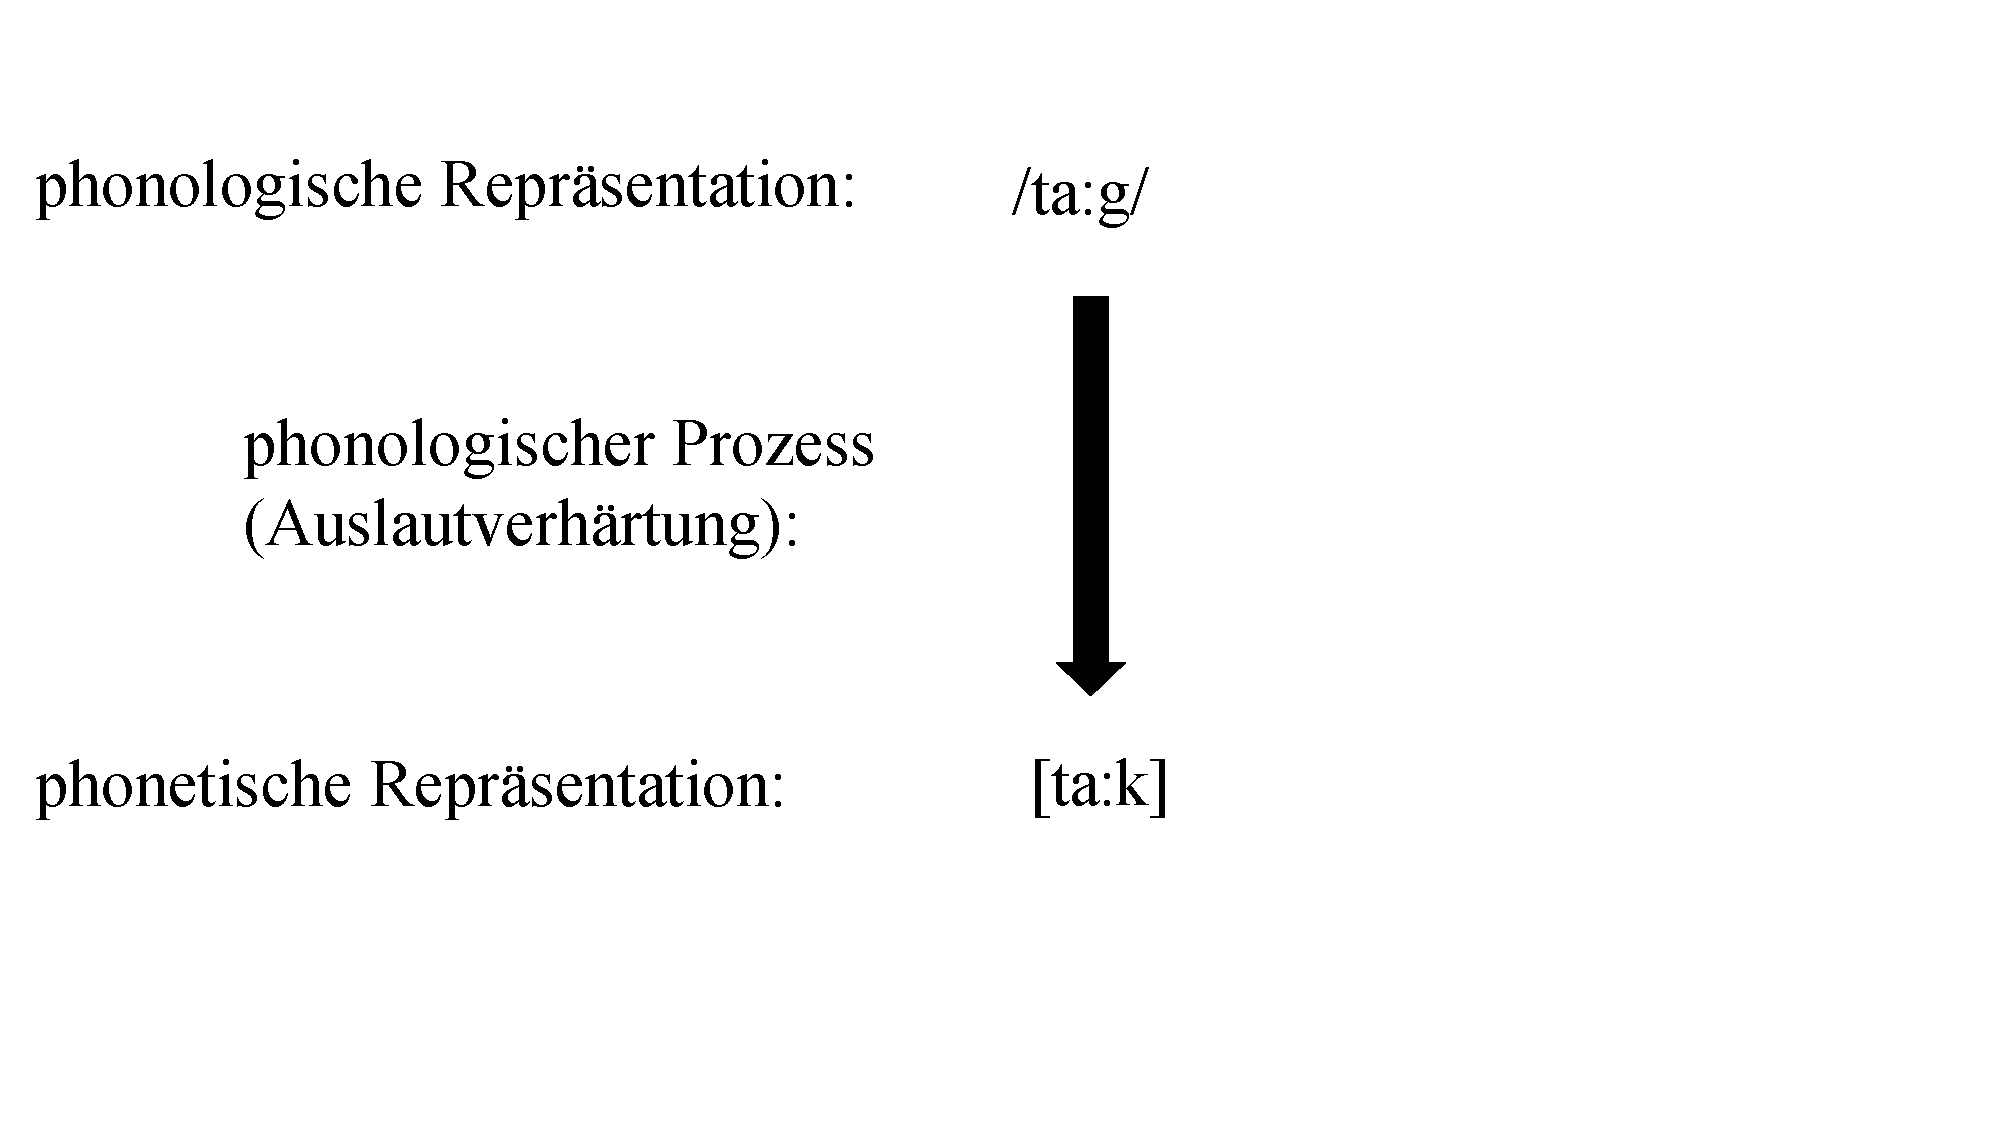
\includegraphics[width=0.5\textwidth]{figures/auslautv.pdf}
    \caption{Wirkung eines phonologischen Prozesses am Beispiel \textit{Tag}\label{fig:phonproz}}
\end{figure}


Wie kommt man zur Annahme einer phonologischen Repräsentation? Wa\-rum geht man nicht einfach davon aus, dass die Singularform \textipa{[ta:k]} genauso im mentalen Lexikon vorhanden ist, und dass als Basis für die Pluralbildung eben die andere Form \textipa{/ta:g/} gespeichert ist? Als Indiz dafür, dass es die phonologische Repräsentation \textipa{/ta:g/} tatsächlich gibt, kann man  Spontanbildungen\is{Spontanbildung} heranziehen. Wenn man mit \textit{Tag} ein neues Wort bilden möchte, etwa mittels eines Adjektivsuffix \textit{-ig} wie in \textit{eklig} oder \textit{-isch} wie in \textit{kindisch} oder mittels des Verbalisierers \textit{-ieren} wie in \textit{telefonieren}, dann wären die resultierenden Formen \textit{tagig, tagisch} und \textit{tagieren}. Alle diese Wörter würden mit \textipa{[g]} gesprochen werden. Es ist nicht möglich, dass Sprecherinnen und Sprecher die Information, genau bei diesen Verbindungen \textipa{[g]} und nicht \textipa{[k]} zu benutzen, irgendwann mal in ihr \is{mentales Lexikon}mentales Lexikon aufgenommen haben, denn sie haben diese Wörter noch nie gehört, sondern gerade spontan gebildet.

Eine \is{phonologische Repräsentation}phonologische Repräsentation enthält laut \citet[63]{Ramers1998} nur die Informationen, die nicht regelhaft vorhersagbar sind. Wie im folgenden Abschnitt~\ref{sec:Auslautverhaertung} genauer ausgeführt wird, gibt es im Deutschen keine stimmhaften Obstruenten in der Koda einer Silbe. Eine Produktion wie \textipa{[ta:g]} ist im Deutschen deshalb nicht möglich. Es werden also regelhaft alle stimmhaften Obstruenten in der Koda entstimmt, sodass diese Information nicht in der phonologischen Repräsentation gespeichert werden muss.


Da \is{Transkription!Klammern}\is{Transkription!Schrägstriche}phonologische Repräsentationen Ab\-straktionen sind, also nicht produziert werden, werden sie wie Phoneme in \is{Transkription!Schrägstriche}Schrägstrichen notiert. Phonetische Repräsentationen sind die Grundlage für Produktionen und werden deshalb wie Phone in eckigen Klammern notiert (vgl. Abbildung~\ref{fig:phonproz})\is{Transkription!Klammern}.

Phonologische Prozesse sind sprachspezifisch. Es wird zum Beispiel nicht in jeder Sprache auslautverhärtet. Beim Erlernen einer Fremdsprache können Sprecherinnen und Sprecher sich zu Beginn nicht (oder nicht sofort) von den phonologischen Prozessen ihrer Erstsprache lösen. Das führt zu einem sprachspezifischen Akzent. Zum Beispiel ist es deutschen Muttersprachlern beim Erlernen des Englischen zu Beginn fast unmöglich, die Wörter \textit{bad} und \textit{bat} erkennbar unterschiedlich zu produzieren, weil sie bei \textit{bad} auslautverhärten.


\begin{Definition}{Phonologische Prozesse}\is{phonologischer Prozess}

\noindent Phonologische Prozesse sind sprachspezifische Ausspracheregeln, die phonologische Repräsentationen in Abhängigkeit vom Kontext in phonetische Repräsentationen überführen.

\end{Definition}


\subsection{Auslautverhärtung}\label{sec:Auslautverhaertung}\is{Auslautverhärtung}

Als erster phonologischer Prozess wird hier die schon erwähnte Auslautverhärtung betrachtet. Bei der Auslautverhärtung werden bestimmte in der phonologischen Repräsentation vorhandene stimmhafte Laute unter bestimmten Bedingungen stimmlos. Es sind also nicht alle stimmhaften Laute betroffen. Beispielsweise wird das \textipa{/d/} bei \textit{danke} nicht stimmlos und das \textipa{/m/} von \textit{Helm} auch nicht. Die Regel der Auslautverhärtung wird deshalb im Folgenden präzisiert. 

Die Auslautverhärtung betrifft im deutschen Standard Obstruenten\is{Obstruent}, also Plosive und Frikative (vgl. Abschnitt~\ref{sec:ObstSon}). Man spricht \textit{Bild} \textipa{[bIlt]}, \textit{schrieb} \textipa{[SKi:p]}, \textit{lag} \textipa{[la:k]}, \textit{brav} \textipa{[bKa:f]} (obwohl die flektierte Form \textit{brave} mit \textipa{[v]} gesprochen wird) und \textit{Gras} \textipa{[gKa:s]} (obwohl bei \textit{Gräser} \textipa{[z]} gesprochen wird). Sonoranten\is{Sonorant} sind von der Auslautverhärtung nicht betroffen. 

In Teilen Süddeutschlands, der Schweiz und Österreich führt die Auslautverhärtung -- anders als im Norddeutschen -- nicht dazu, dass Wörter wie \textit{bunt} und \textit{Bund} identisch klingen. Die Sprecherinnen und Sprecher unterscheiden \textit{Bund} und \textit{bunt} akustisch dadurch, dass der finale Konsonant in \textit{Bund} kürzer und der Vokal vor dem Konsonanten länger als in \textit{bunt} ist \citep[72]{DudenAussprache2023}.

Im norddeutschen Sprachraum wirkt sich die Auslautverhärtung, wie \citet[242]{Hall2000} zeigt, auf Obstruenten \textit{in der Koda einer Silbe} aus. Die Auslautverhärtung gibt es also wortfinal wie in den Beispielen oben, aber auch silbenfinal wie bei \textit{Erbse} \textipa{[\textprimstress PE5p.z@]}, \textit{Schreibtisch} \textipa{[\textprimstress SK\t*{aI}p.tIS]}, \textit{täglich} \textipa{[\textprimstress te:k.lI\c{c}]} oder sogar als nichtfinaler Konsonant in der Koda, etwa bei \textit{Jagd} \textipa{[ja:kt]}, wo die letzten beiden Konsonanten betroffen sind, oder \textit{lobt} \textipa{[lo:pt]}, wo der letzte Konsonant schon stimmlos ist, der vorletzte aber durch die Auslautverhärtung entstimmt wird.


\begin{Definition}{Auslautverhärtung}\is{Auslautverhärtung}

\noindent Die Auslautverhärtung ist ein \isi{phonologischer Prozess}, durch welchen zugrundeliegende stimmhafte Obstruenten in der \is{Koda}Koda einer Silbe stimmlos werden.

\end{Definition}


Die Auslautverhärtung ist im norddeutschen Standard ein obligatorischer Prozess\is{phonologischer Prozess! obligatorisch}. Das bedeutet, dass Sprecherinnen und Sprecher nicht wählen können, ob sie die Auslautverhärtung durchführen oder nicht.

Wie alle phonologischen Prozesse ist auch die Auslautverhärtung sprachspezifisch. Im Russischen und Türkischen wird ebenfalls auslautverhärtet. Im Englischen und Französischen wird jedoch nicht auslautverhärtet (vgl. Beispiele (\ref{EnglischAuslaute}) bis (\ref{RussischAuslautverhaertung}) auf Seite \pageref{EnglischAuslaute} in Kapitel~\ref{kap:Graphematik}).


\subsection{Epenthese}\label{sec:Epenthese}\is{Epenthese}

Unter einer Epenthese versteht man die Einfügung eines Segments, etwa wenn Sprecherinnen und Sprecher das Wort \textit{Hemd} \textipa{[hEmpt]} statt \textipa{[hEmt]} sprechen. Die Einfügung von \textipa{[p]} entsteht hier durch eine zeitliche Verschiebung der Bewegungen von Velum, Lippen und Zungenspitze. Um vom \textipa{[m]} zum \textipa{[t]} überzugehen, muss das Velum angehoben und die Lippen müssen geöffnet werden. Vor der Öffnung der Lippen muss jedoch der alveolare Verschluss für \textipa{[t]} produziert werden. Wenn das Velum angehoben wird und die Lippen geöffnet werden, der alveolare Verschluss aber noch nicht gebildet wurde, entsteht ein bilabialer Plosiv. Andere Beispiele für Epenthesen sind die Einsetzung\is{phonologischer Prozess!fakultativ} von \textipa{[p]} bei \textipa{[kOmpt]} für \textit{kommt} oder die \textipa{[t]}-Epenthese beim Genitiv von \textit{Leben, Lebens} \textipa{[\textprimstress le:b@nts]}.

Während die bisher angesprochenen Epenthesen fakultativ sind, ist die \is{Knacklaut-Epenthese}Knacklaut-Epenthese im Standard obligatorisch. Der Knacklaut \textipa{[P]} wird \citet[65]{Hall2000} zufolge im Onset einer Silbe platziert, wenn

\begin{itemize}
    \item dort kein weiteres Segment steht \textit{und}
    \item die Silbe betont ist oder wenn es sich um die erste Silbe eines Wortes handelt (vgl. Abschnitt~\ref{subsection:Plosive}).
\end{itemize}

Die \is{phonologische Repräsentation}phonologische Repräsentation des Wortes \textit{Amt} ist also \textipa{/amt/}. Über die Knacklaut-Epenthese kommt man zur \is{phonetische Repräsentation}phonetischen Repräsentation \textipa{[Pamt]}, denn der Onset der ersten (und einzigen) Silbe des Wortes ist leer. Bei \textit{Beamte} wird der Knacklaut am Anfang der zweiten Silbe eingesetzt, denn diese Silbe ist betont und ihr Onset wäre sonst leer. Die phonologische Repräsentation ist also \textipa{/b@\textprimstress am.t@/}, die phonetische ist \textipa{[b@\textprimstress Pam.t@]}.\footnote{Bei \textit{bauen} wird hingegen kein Knacklaut eingesetzt, obwohl die zweite Silbe einen leeren Onset hat. Das liegt daran, dass diese Silbe unbetont ist.}




\subsection{\textipa{/K/}-Vokalisierung}\is{R-Vokalisierung@\textipa{/K/}-Vokalisierung}
\label{subsec:r-Vokalisierung}

Bei der \textipa{/K/}-Vokalisierung wird ein \textipa{/K/}, welches in der Koda einer Silbe steht, zum tiefen Schwa \textipa{[5]}. Wir schauen uns dazu das Wort \textit{Tier} mit seiner Pluralform \textit{Tiere} an. Die phonologische Repräsentation\is{phonologische Repräsentation} von \textit{Tier} ist \textipa{/ti:K/}. Die Silbenstruktur der phonologischen Repräsentation von \textit{Tier} ist in Abbildung~\ref{Silbenstruktur_Tier} darstellt. Das \textipa{/K/} steht hier in der Koda und wird deshalb vokalisiert. Es entsteht die phonetische Repräsentation\is{phonetische Repräsentation} \textipa{[ti:5]} oder auch als Diphthong \textipa{[t\t*{i5}]}, die in Abbildung~\ref{Silbenstruktur_Tier_vokalisiert} dargestellt ist. Das tiefe Schwa ist jetzt Bestandteil des Nukleus.\footnote{Phonologisch betrachtet müsste man für den ursprünglichen Nukleus \textipa{/i:/} zwei X-Positionen vorsehen, sodass insgesamt drei X-Positionen im Nukleus stehen. Phonetisch betrachtet bildet das \textipa{/i:/} aber nun mit dem tiefen Schwa zusammen einen Diphthong. Diphthonge besetzen zusammen nur zwei X-Positionen.}

\begin{figure}[!htbp]
  \centering
  \begin{forest}
[σ 
        [Onset, ake 
          [X [\textipa{t}]]
        ]
       [Reim 
         [Nukleus 
           [X, name=ERBaum]
           [X
                [\textipa{i:}]
                {\draw[-] (.north) -- (ERBaum.south);}
            ]
        ] 
          [Koda, ake
            [X [\textipa{K}]]
          ]
      ] 
] 
  \end{forest}
  \caption{Konstituentenanalyse der phonologischen Repräsentation von \textit{Tier}: Der r-Laut steht in der Koda.}
  \label{Silbenstruktur_Tier}
\end{figure}

Bei der Pluralform \textit{Tiere} wird, wie in Abbildung~\ref{Silbenstruktur_Tiere} dargestellt, nicht vokalisiert, weil das \textipa{/K/} nicht in der Koda, sondern im Onset steht.

\begin{figure}[!htbp]
  \centering
  \begin{forest}
[σ 
        [Onset, ake 
          [X [\textipa{t}]]
        ]
        [Reim 
         [Nukleus
           [X
                [\textipa{i}]
            ]
            [X
                [\textipa{5}]
            ]
        ] 
          [Koda, ake
          ] 
      ] 
] 
  \end{forest}
  \caption{Konstituentenanalyse von \textit{Tier} mit Vokalisierung. Der vokalisierte r-Laut (tiefes Schwa) steht im Nukleus. \label{Silbenstruktur_Tier_vokalisiert}}
\end{figure}



\begin{figure}[!htbp]
  \centering
  \begin{forest}
  [Wort
      [σ, calign=last
        [Onset, ake
          [X [\textipa{t}]]
        ]
      [Reim, calign=first
          [Nukleus, ake
          [X, name=ERBaum]
    [X [\textipa{i:}]
    {\draw[-] (.north) -- (ERBaum.south);}
    ]
          ]
          [Koda,
      ]
      ]
      ]
      [σ, calign=last
      [Onset, ake
          [X [\textipa{K}]]
        ]
        [Reim
          [Nukleus, ake
            [X [\textipa{@}]]
          ]
          [Koda
          ]
        ]
      ]
    ]
  \end{forest}
  \caption{Konstituentenanalyse von \textit{Tiere}: Der r-Laut steht im Onset der zweiten Silbe und wird nicht vokalisiert.}
  \label{Silbenstruktur_Tiere}
\end{figure}

Die \textipa{/K/}-Vokalisierung ist \citet[144]{Noske1993} zufolge obligatorisch nach gespannten Vokalen, \zB in \textit{wir, Ohr, wer}, und fakultativ nach ungespannten, \zB in \textit{wirr, Ort, werfen}. Laut \citet[856f]{Duden2022} jedoch wird jedes \textipa{/K/} in der Koda vokalisiert, also auch nach ungespannten Vokalen wie in \textit{wirr, Herr, dürr} \textipa{[vI5, hE5, dY5]}. Das \citet{DudenAussprache2023} wiederum sieht nach ungespanntem Vokal keine \textipa{/K/}-Vokalisierung vor: \textipa{[vIr, hEr, dYr]}. Das \citet[140]{DudenZweifelsfaelle2021} empfiehlt ebenfalls, nach ungespannten Vokalen auf die \textipa{/K/}-Vokalisierung zu verzichten. 

Unterschiedliche Arten der Realisierung gibt es außerdem nach \textipa{/a/}. Während die \citet[857]{Duden2022} auch dort eine Vokalisierung vorsieht, \zB bei \textit{Star} \textipa{[Sta:5]} und \textit{starr} \textipa{[Sta5]}, gibt das \citet[819]{DudenAussprache2023} \textipa{[Sta:]} und \textipa{[Star]} an.


\subsection{Schwa-Tilgung}\label{sec:Schwatilgung}\is{Schwa-Tilgung}

Der \is{Laute!Schwa}Schwa-Laut \textipa{/@/} ist \citet[106]{KoherlRodgers2001} zufolge der häufigste Vokal im Deutschen. Er tritt ausschließlich in unbetonten Silben auf. Durch das im Deutschen vorherrschende \is{Trochäus}trochäische Betonungsmuster findet man ihn meist in der Silbe, die der betonten Silbe folgt, etwa in \textit{Mantel} \textipa{/\textprimstress man.t@l/}, \textit{bitten} \textipa{/\textprimstress bI\.*{t}@n/}, \textit{müssen} \textipa{/\textprimstress mY\.*{s}@n/}, \textit{rasen} \textipa{/\textprimstress ra:.z@n/}, \textit{malen} \textipa{/\textprimstress ma:.l@n/}, \textit{mahnen} \textipa{/\textprimstress ma:.n@n/}, \textit{bauen} \textipa{/baU.@n/}, \textit{ihrem} \textipa{/\textprimstress i:.K@m/}. Aber auch in Wörtern mit \is{Präfix}Präfix, etwa in \textit{gelingen} \textipa{/g@\textprimstress lI\.*N@n/}, \textit{besichtigen} \textipa{/b@\textprimstress zI\c{c}.tig@n/} usw. tritt er auf.

Prinzipiell kann das Schwa in der Standardlautung getilgt werden (d.\,h. entfallen), wenn der Folgekonsonant ein Sonorant ist \citep[41ff]{DudenAussprache2023}. Dieser Sonorant wird dabei silbisch\is{Transkription!silbischer Konsonant}, er übernimmt also die Funktion des Nukleus. \is{Transkription!silbischer Konsonant}In der Transkription kennzeichnet man das durch einen kleinen Strich unter dem Konsonanten. Bei \textit{Mantel} wird aus der phonologischen Repräsentation \textipa{/\textprimstress man.t@l/} durch die Schwa-Tilgung die phonetische Repräsentation \textipa{[\textprimstress man.t\s{l}]} mit silbischem \textipa{[l]}. Weitere Beispiele für Schwa-Tilgungen sind \textit{bitten} \textipa{[\textprimstress bI\.*{t}\s{n}]}, \textit{müssen} \textipa{[\textprimstress mY\.*{s}\s{n}]} , \textit{rasen} \textipa{[\textprimstress ra:.z\s{n}]}, \textit{malen} \textipa{[\textprimstress ma:.l\s{n}]}, \textit{mahnen} \textipa{[\textprimstress ma:.n\s{n}]}, \textit{bauen} \textipa{[\textprimstress baU.\s{n}]}, \textit{ihrem} \textipa{[\textprimstress Pi:.K\s{m}]} (oft mit Resilbifizierung und \textipa{/K/}-Vokalisierung: \textipa{[Pi:5m]}).

Wenn der Folgelaut kein Sonorant ist, erfolgt keine Schwa-Tilgung: \textit{bittet} \textipa{[\textprimstress bI\.*{t}@t]}, nicht: \textipa{[\textprimstress bIt.t]}, \textit{ratloses} \textipa{[\textprimstress Ka:t.lo.z@s]}, nicht: \textipa{[\textprimstress Ka:t.lo.zs]}.

Die \is{Schwa-Tilgung}Schwa-Tilgung ist immer optional. Ob ein Schwa vor Sonorant wirklich getilgt wird, hängt nicht nur vom Folgelaut, sondern auch vom Register,\footnote{Unter \textit{Register} versteht man den Sprachgebrauch, der für eine bestimmte Kommunikationssituation charakteristisch ist, etwa Kommunikation  mit Kindern, Kommunikation in formellen Situationen usw. \citep{Halliday1978}.}\is{Register} vom Sprechtempo, vom vorangehenden Laut und der Position der Schwa-Silbe ab. \citet[101]{KoherlRodgers2001} zeigen für norddeutsche Sprecherinnen und Sprecher, dass die Schwa-Tilgung in Spontansprache häufiger ist als in gelesener Sprache. Während in gelesener Sprache 44\% von allen Schwas getilgt wurden, wurden in spontaner Sprache 64\% getilgt \citep[104]{KoherlRodgers2001}. Außerdem wird das Schwa häufiger nach Nasalen, Liquiden und Vokalen getilgt als nach Frikativen. Man kann also eher eine Tilgung bei Wörter wie \textit{mahnen, malen, bauen} erwarten als in Wörtern wie \textit{rasen, müssen}. Wenn die Silbe mit dem Schwa der betonten Silbe vorangeht (zum Beispiel in \textit{gelingen}) wird das Schwa seltener getilgt, als wenn die Silbe mit dem Schwa der betonten Silbe folgt.


\subsection{Assimilation}\label{subsection:Assimilation}\is{Assimilation}

Bei der Assimilation beeinflusst ein Laut einen benachbarten so, dass der beeinflusste Laut sich in einer oder mehreren Merkmalen an den beeinflussenden Laut angleicht \citep[89]{Hall2000}. Abbildung~\ref{fig:regNasalass} stellt eine Assimilation beim  Wort \textit{Rennbahn} dar. Die phonologische Repräsentation ist \textipa{/\textprimstress KEn\textsecstress ba:n/}. Über die Assimilation kann daraus in spontanter Sprache \textipa{[\textprimstress KEm\textsecstress ba:n]} werden \citep{Zimmereretal:2009}.\is{Nasalassimilation}

\begin{figure}
    \centering
    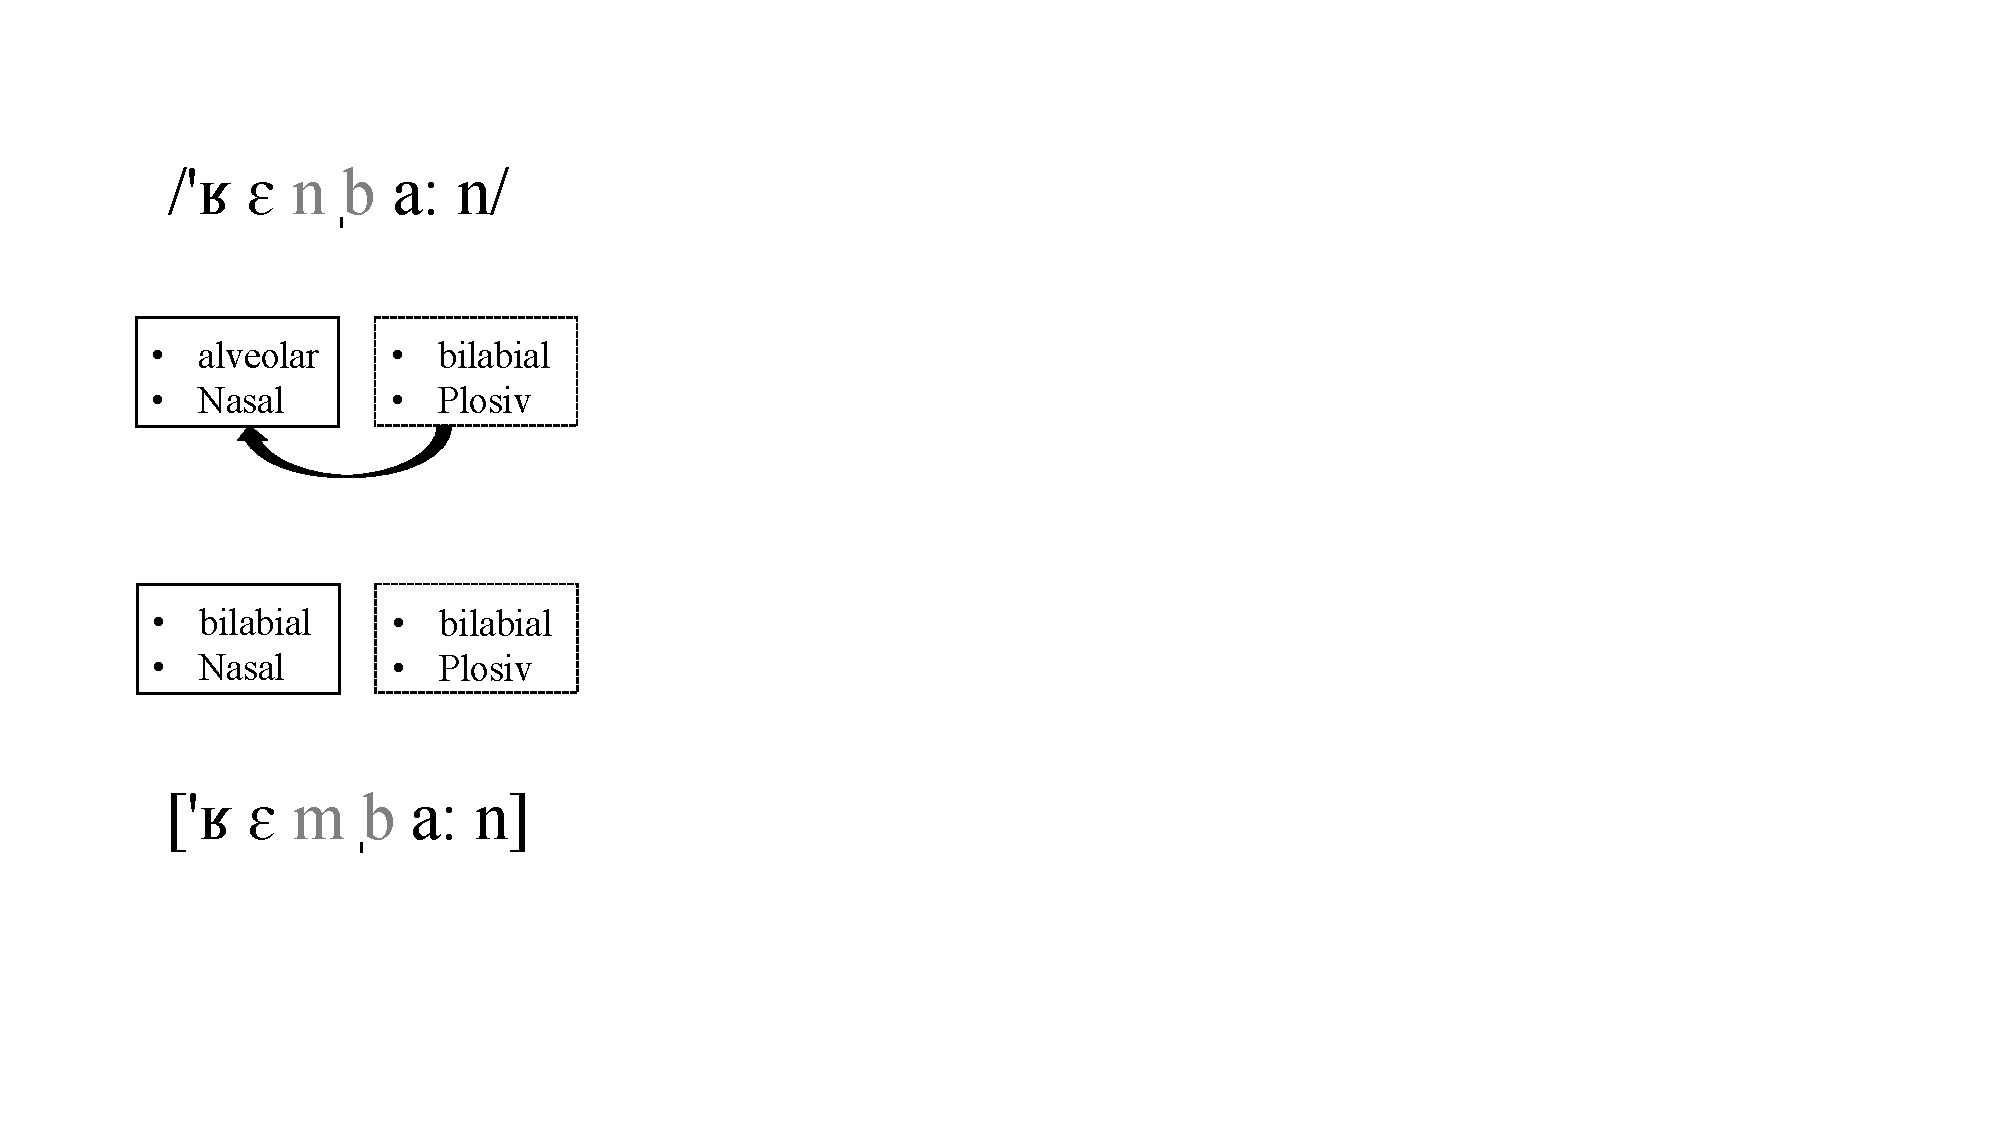
\includegraphics[width=0.4\textwidth]{figures/assimilation.pdf}
    \caption{Regressive Nasalassimilation \label{fig:regNasalass}}
\end{figure}

Der beeinflusste Laut, das \textipa{/n/} in der \is{phonologische Repräsentation}phonologischen Repräsentation, ist ein alveolarer Nasal (oberes linkes Kästchen in der Abbildung). Der beeinflussende Laut, das \textipa{/b/}, ist ein bilabialer Plosiv (oberes rechtes Kästchen in der Abbildung). Der Plosiv überträgt seinen Artikulationsort \textit{bilabial} auf den Nasal, sodass dieser zum bilabialen Nasal \textipa{[m]} wird (unteres linkes Kästchen).

Eine\is{Assimilation!regressiv}\is{Assimilation!progressiv} Assimilation wie bei \textipa{/nb/} zu \textipa{[mb]}, bei der der Folgelaut den vorangehenden beeinflusst, nennt man \textit{regressive Assimilation} (auch \textit{anticipatory assimilation}). Bei einer \textit{progressiven Assimilation} (auch \textit{carry over assimilation}) beeinflusst der vorangehende Laut den folgenden. Progressive Assimilationen kommen häufig nach einer Schwa-Tilgung vor, etwa bei dem Wort \textit{haben}. Die phonologische Repräsentation ist \textipa{/\textprimstress ha:.b@n/}. Dann kann eine Schwa-Tilgung erfolgen, sodass \textipa{[\textprimstress ha:.b\s{n}]} entsteht. Erst dann kann assimiliert werden, indem das \textipa{/b/} seinen Artikulationsort auf das \textipa{/n/} überträgt, sodass \textipa{[\textprimstress ha:.b\s{m}]} entsteht. Laut \citet[69f]{DudenAussprache2023} treten progressive Assimilationen wie in \textipa{[\textprimstress ha:b\s{m}]} im Standarddeutschen auf, sie sind aber nicht obligatorisch.

Weitere Beispiele für die Nasalassimilation diskutiert \citet[Kap. 4]{Hall1992}. Einige davon sind in Tabelle~\ref{tab:Assimilation} wiedergegeben. Bei \textit{Becken} (erstes Beispiel in der Tabelle) wird zunächst der Schwa-Laut getilgt: \textipa{[\textprimstress bE\.*{k}\s{n}]}. Dann erfolgt eine progressive Assimilation. Der velare Plosiv überträgt sein Ortsmerkmal auf den ursprünglich alveolaren Nasal. Es entsteht die phonetische Repräsentation \textipa{[\textprimstress bE\.*k\s{N}]}. Das Beispiel \textit{legen} ist vergleichbar. Zunächst wird das Schwa getilgt, dann überträgt das \textipa{/g/} sein Ortsmerkmal auf den Nasal.

Von einer Assimilation spricht man auch, wenn ein Merkmal nur teilweise übertragen wurde, wie etwa bei \textit{Senf} (drittes Beispiel in der Tabelle). Hier ist der beeinflussende Laut, das \textipa{/f/}, ein labiodentaler Laut. Durch die Assimilation wird der vorangehende Laut \textipa{/n/} nicht notwendigerweise labiodental, aber zumindest labial. Anschließend kann eine Epenthese erfolgen, sodass die phonetische Repräsentation \textipa{[zEmpf]} entsteht.

Bei \textit{Angriff} (viertes Beispiel) erfolgen eine \textipa{[P]}-Epenthese und eine regressive Assimilation. Das \textipa{/g/} überträgt sein Ortsmerkmal auf den vorangehenden Nasal. Im Unterschied zum ersten bis dritten Beispiel in der Tabelle, wo der erste Prozess erst die Voraussetzungen für den zweiten Prozess schafft, sind die beiden Prozesse beim vierten Beispiel unabhängig voneinander. Man kann also genauso gut annehmen, dass zuerst die Assimilation und dann die \textipa{[P]}-Epenthese erfolgt.

\footnotesize
\begin{table}
\centering
\caption{Beispiele für Assimilationsprozesse im Deutschen in Kombination mit anderen phonologischen Prozessen\label{tab:Assimilation}}
\begin{tabular}{lllll}\lsptoprule
Orthograf. & Phonolog.&1. Phonolog. & 2. Phonolog. & Phonet. \\
Form & Repräs.& Prozess & Prozess & Repräs.\\\midrule
\textit{Becken} & \textipa{/\textprimstress bE\.*k@n/} & Schwa-Tilgung & prog. Assim. & \textipa{[\textprimstress bE\.*k\s{N}]}\\
\textit{legen} & \textipa{/\textprimstress le:.g@n/} & Schwa-Tilgung & prog. Assim. & \textipa{[\textprimstress le:.g\s{N}]}\\
\textit{Senf} & \textipa{/zEnf/} & reg. Assim. & Epenthese&  \textipa{[zEmpf]}\\
\textit{Angriff} & \textipa{/\textprimstress an.gKIf/} & \textipa{[P]}-Epenthese & reg. Assim. & \textipa{[\textprimstress PaN.gKIf]}\\
\lspbottomrule
\end{tabular}
\end{table}

\normalsize

Auch die \isi{Stimmhaftigkeit} kann assimiliert werden, beispielsweise wenn auf stimmlose Plosive ein Liquid folgt wie bei \textit{Kleid} oder \textit{Kraut}, wo das \textipa{/l/} bzw. \textipa{/K/} stimmlos gesprochen werden, weil sie dieses Merkmal von den vorangegangenen Plosiven übernehmen \citep[70]{FuhrhopPeters2013}. Der Unterschied im Onset der ersten Silbe von \textit{Kleid} und \textit{gleiten} liegt also gar nicht in der Artikulation von \textipa{/k/} vs \textipa{/g/}, sondern darin, dass das \textipa{/l/} bei \textit{Kleid} stimmlos und bei \textit{gleiten} stimmhaft ist. Ebenso besteht der Unterschied in den Onsets von \textit{Kraut} und \textit{grau} nicht darin, dass der Plosiv anders gesprochen wird, sondern darin, dass das \textipa{/K/} bei \textit{Kraut} stimmlos und bei \textit{grau} stimmhaft ist.

Die bisher diskutierten Assimilationen betrafen immer benachbarte Laute. Es gibt jedoch auch sogenannte \is{Fernassimilation}Fernassimilationen \citep[71]{FuhrhopPeters2013}. Im Deutschen ist der \is{Umlaut}Umlaut ein Resultat einer solchen Fernassimilation. Zu Beginn dieses Sprachwandelprozesses trat der a-Umlaut \textipa{[E]}  nur in Wörtern auf, die in der Folgesilbe ein \textipa{/i/} oder \textipa{/j/} enthielten. Beispielsweise war der Plural des althochdeutschen Wortes \textit{gast}\footnote{im Neuhochdeutschen \textit{Gast}} \textit{gasti}. Der Vokal der ersten Silbe \textipa{/a/} wurde an den Vokal der zweiten Silbe assimiliert, indem er nach und nach mit immer höherer Zungenposition gesprochen wurde. Aus \textipa{[gasti]} wurde \textipa{[gEsti]}, der Vorläufer des neuhochdeutschen Wortes \textit{Gäste} \citep[40]{Nuebling_et_al_2017}.

Assimilationen sind sehr häufig, die wenigsten sind aber für den Standard obligatorisch. Obligatorisch ist die Assimilation der Stimmhaftigkeit etwa bei \textit{Kleid} und \textit{Kraut}. Ebenfalls obligatorisch sind die Assimilationen des alveolaren Nasals \textipa{/n/} vor velaren Plosiven wie \textipa{/k/}, wenn keine Morphemgrenze dazwischen liegt, etwa  bei \textit{Bank}: \textipa{[baNk]}, statt ohne Assimilation \textipa{[bank]}.\footnote{Diese Analyse setzt voraus, dass man \textipa{[N]} nicht als Phonem betrachtet \citep[66f]{Hall2000}.} Fakultativ ist diese Assimilation, wenn zwischen \textipa{/n/} und dem Plosiv eine Morphemgrenze liegt, etwa bei \textit{Angriff} (vgl. Tabelle~\ref{tab:Assimilation}). Die regressive Nasalassimilation von \textipa{/n/} vor \textipa{/f/}, \zB bei \textit{fünf} \textipa{[fYnf]} zu \textipa{[fYmf]} wird vom \citet[139]{DudenZweifelsfaelle2021} sogar abgelehnt.

\subsection{\textipa{/g/}-Tilgung}\is{g-Tilgung@/g/-Tilgung}\label{sec:gTilgung}

Vor allem in Norddeutschland hört man Produktionen wie \textipa{[dINk]} für \textit{Ding}  oder \textipa{[\textprimstress PaX.tUNk]}\footnote{Im Ausspracheduden verzeichnet die Transkription von \textit{Achtung} keinen Knacklaut, weil der Knacklaut regelhaft gesetzt wird und deshalb im Ausspracheduden am Wortanfang vor Vokal nicht vermerkt wird \citep[14]{DudenAussprache2023}.} für \textit{Achtung} \citep[70]{DudenAussprache2023}. Diese Varianten sind das Resultat einer regressiven Nasalassimilation des \textipa{/n/} an das \textipa{/g/}, gefolgt von einer Auslautverhärtung: \textipa{/dIng/} \rightarrow \textipa{[dINg]} \rightarrow \textipa{[dINk]}.

Standardsprachlich wird laut Ausspracheduden statt der Auslautverhärtung aber eine sogenannte \textipa{/g/}-Tilgung durchgeführt, sodass sich die Aussprache \textipa{[dIN]} ergibt \citep[321]{DudenAussprache2023}. Bei einer \textipa{/g/}-Tilgung entfällt \textipa{/g/}, wenn 
\begin{itemize}
    \item dem \textipa{/g/} ein \textipa{/n/} vorangeht \textit{und}
    \item das \textipa{/g/} in der Koda einer Silbe steht \textit{und}
    \item dem \textipa{/g/} kein gespannter Vokal folgt.
\end{itemize}


Jeder \textipa{/g/}-Tilgung geht eine Assimilation des \textipa{/n/} an das \textipa{/g/} voraus. Die Beispiele in Tabelle~\ref{tab:gTilgung} sind \citet[818--819, 823]{Hall1989} entnommen. Wir diskutieren zunächst die ersten fünf Beispiele, bei denen eine \textipa{/g/}-Tilgung erfolgt, und dann das letzte, bei dem keine \textipa{/g/}-Tilgung stattfindet.

\begin{table}
\centering
\caption{Beispiele für \textipa{/g/}-Tilgungen nach Assimilation\label{tab:gTilgung}}
\begin{tabular}{llll}\lsptoprule
Orthografische & Phonologische&1. Prozess:& 2. Prozess: \\
Form & Repräsentation & Assimilation & \textipa{/g/}-Tilgung\\\midrule
\textit{lang} & \textipa{/lang/} & \textipa{[laNg]}  & \textipa{[laN]} \\
\textit{Hengst} & \textipa{/hEngst/} & \textipa{[hENgst]} & \textipa{[hENst]}\\
\textit{länglich} & \textipa{/\textprimstress lEnglI\c{c}/} & \textipa{[\textprimstress lENglI\c{c}]}  & \textipa{[\textprimstress lEN.lI\c{c}]}\\
\textit{Sprengung} & \textipa{/\textprimstress SpKEngUng/} & \textipa{[\textprimstress SpKENgUNg]} & \textipa{[\textprimstress SpKE\.*{N}UN]}\\
\textit{Mangel} & \textipa{/\textprimstress mang@l/} & \textipa{[\textprimstress maNg@l]} & \textipa{[\textprimstress ma\.*{N}@l]}\\
\textit{Tango} & \textipa{/\textprimstress tango/} & \textipa{[\textprimstress taNgo]} & --\\
\lspbottomrule
\end{tabular}
\end{table}

Die phonologische Repräsentation des ersten Beispiels in der Tabelle, \textit{lang}, enthält ein \textipa{/ng/} in der Koda. Als erster phonologischer Prozess erfolgt eine Assimilation, sodass aus dem \textipa{/n/} durch den Einfluss des \textipa{/g/} ein \textipa{[N]} wird. Im zweiten Schritt wird das \textipa{/g/} getilgt. Beim zweiten Beispiel, \textit{Hengst}, steht das \textipa{/g/} nicht in wortfinaler Position. Da es aber trotzdem in der Koda nach \textipa{/n/} steht, erfolgen dieselben zwei Prozesse. Auch bei den Zweisilbern \textit{länglich}, \textit{Sprengung} und \textit{Mangel}, erfolgt eine \textipa{/g/}-Tilgung nach Assimilation, bei \textit{Sprengung} sogar zweimal. Zur Frage, warum das \textipa{/g/} bei \textit{Sprengung }und \textit{Mangel} eigentlich getilgt wird, obwohl es in der phonologischen Repräsentation scheinbar nicht in der Koda der ersten Silbe steht, sondern im Onset der zweiten vgl. Exkurs~\ref{ex:gTilgung}.

\textit{Tango} scheint von seiner lautlichen Struktur her dem Wort \textit{Mangel} sehr ähnlich zu sein. Aber im Gegensatz zu \textit{Mangel} enthält die zweite Silbe von \textit{Tango} einen gespannten Vokal, das \textipa{/o/}. Wenn ein solcher Vokal in der Folgesilbe auftritt, kommt es nicht zu einer \textipa{/g/}-Tilgung. Aus demselben Grund wird bei den Vornamen \textit{Inge} und \textit{Ingo} einmal getilgt und einmal nicht. Bei \textit{Inge} \textipa{[PI\.*N@]} wird das \textipa{/g/} getilgt, weil der Vokal der zweiten Silbe ein Schwa ist, bei \textit{Ingo} \textipa{[PIN.go]} wird das \textipa{[g]} gesprochen, weil der Vokal der zweiten Silbe ein gespannter Vokal ist. Genauso spricht man \textit{Menge} ohne \textipa{[g]}, weil in der Folgesilbe ein Schwa-Laut steht, aber \textit{Mango} mit \textipa{[g]}, weil die Folgesilbe einen gespannten Vokal enthält. 


\begin{Exkurs}{Steht das \textipa{/g/} bei \textit{länglich}, \textit{Sprengung} und \textit{Mangel}\\ tatsächlich in der Koda?}\label{ex:gTilgung}\is{Suffigierung}\is{Silbifizierung}

Nach der Sonorität zu urteilen, müsste das \textipa{/g/} in der phonologischen Repräsentation von \textit{länglich} eigentlich im Onset der zweiten Silbe stehen: \textipa{/\textprimstress lEn.glI\c{c}/}. Das würde bedeuten, dass es nicht getilgt werden kann, denn die \textipa{/g/}-Tilgung betrifft nur Koda-Konsonanten. Die Silbengrenze ist hier aber identisch mit der morphologischen Grenze, \textipa{/\textprimstress lEng.lI\c{c}/}, weil Suffixe mit besetztem Onset keine Resilbifizierung hervorrufen \citep[73]{Bergmann2018}. So silbifiziert man \textit{kind-lich} statt \textit{kin-dlich}, \textit{Prüf-ling} statt \textit{Prü-fling} und \textit{Er-leb-nis} statt \textit{Er-le-bnis}. Das \textipa{/g/} bei \textit{länglich} steht also in der Koda und wird getilgt.\is{g-Tilgung@/g/-Tilgung}

Das Suffix \textit{-ung} in \textit{Sprengung} hat vor der Suffigierung einen leeren Onset. Solche Suffixe lösen eine Resilbifizierung\is{Resilbifizierung} aus, bei der mindestens der letzte Konsonant des Stammes in die Silbe des Suffixes übergeht \citep[813]{Hall1989}. Beispiele, die diese Resilbifizierung zeigen, sind \textit{Lö-sung, Ü-bung, Lei-tung} (statt \textit{Lös-ung, Üb-ung, Leit-ung}).\footnote{Das Beispiel \textit{Han-dlung} zeigt, dass ein Suffix mit unbesetzem Onset sogar mehrere Konsonanten in die Folgesilbe ziehen kann. \citet[815]{Hall1989} zufolge passiert das bei Suffixen mit leerem Onset, wenn der Stamm, mit welchem sie sich verbinden, auf Konsonant+Sonorant auslautet. Ob die Silbifizierung tatsächlich \textit{Han-dlung} ist, erkennt man daran, ob das \textipa{/d/} auslautverhärtet wird. Ohne Auslautverhärtung steht es im Onset: \textipa{[\textprimstress han.dlUN]}, mit Auslautverhärtung in der Koda: \textipa{[\textprimstress hant.lUN]}} Demzufolge müsste die phonologische Repräsentation von \textit{Sprengung} eigentlich \textipa{/SpKEn.gUng/} silbifiziert werden. Dann stände das \textipa{/g/} nicht mehr in der Koda und würde nicht getilgt werden. \citet[819--820]{Hall1989} argumentiert jedoch, dass die phonologischen Prozesse, also die Assimilation und die \textipa{/g/}-Tilgung, der Resilbifizierung durch das Suffix vorangehen. Es gibt also zunächst einen Stamm und ein Affix: \textipa{/SpKEng/}, \textipa{/Ung/}. Diese verbinden sich \newline-- zunächst ohne Resilbifizierung -- zu \textipa{/SpKEng.Ung/}. Dann erfolgen die phonologischen Prozesse (Assimilation und \textipa{/g/}-Tilgung), sodass \textipa{[SpKEN.UN]} entsteht. Und erst dann wird resilbifiziert: \textipa{[\textprimstress SpKE\.*{N}UN]}. Zu dem Zeitpunkt, zu welchem das \textipa{/g/} in die Silbe des Suffixes wechseln sollte, existiert es also gar nicht mehr. Für den Onset der zweiten Silbe kommt nur noch ein \textipa{[N]} in Frage, und da dieser Laut einem Kurzvokal in betonter Silbe folgt, wird er ambisilbisch (Silbengelenk).

Anders ist das bei \textit{Mangel}. Dieses Wort ist morphologisch einfach. Man kann also nicht argumentieren, dass die Besetzung des Onsets der zweiten Silbe erst erfolgt, wenn das \textipa{/g/} schon getilgt ist. Das Wort \textit{Mangel} sollte also vergleichbar sein mit \textit{Tango}, wo zwar assimiliert wird, das \textipa{/g/} dann aber nicht getilgt wird, weil es nicht in der Koda, sondern im Onset der nächsten Silbe steht. \citet[823--830]{Hall1989} erklärt dieses Phänomen, indem er annimmt, dass der Schwa-Laut kein zugrundeliegender Laut ist, sondern immer Resultat einer Epenthese. Wenn man von einer phonologischen Repräsentation \textipa{/mangl/} ausgeht, steht das \textipa{/g/} in der Koda und wird getilgt.

\end{Exkurs}

Die \textipa{/g/}-Tilgung ist unter den genannten Bedingungen im Standard obligatorisch, d.\,h. man kann sie nicht weglassen. Allerdings kann man sie -- wie zu Beginn des Abschnittes gezeigt -- in finaler Position durch eine Auslautverhärtung ersetzen, also \textipa{[laNk, hENkst]} für \textit{lang, Hengst} sprechen. Von einigen Sprecherinnen und Sprechern wird diese Variante aber nicht als standardgemäß angesehen. Auch das \citet[138]{DudenZweifelsfaelle2021} empfiehlt diese Aussprache nicht. 

Am Beispiel der \textipa{/g/}-Tilgung kann man -- wie schon beim Prozess der Auslautverhärtung -- zeigen, dass phonologische Prozesse sprachspezifisch sind: Die \textipa{/g/}-Tilgung existiert im Deutschen, aber \zB nicht im Englischen. Das Wort \textit{Englisch} etwa wird im Deutschen ohne \textipa{[g]} gesprochen, \textipa{[\textprimstress PEN.lIS]}, im Englischen spricht man das Wort \textit{English} aber mit \textipa{[g]}, da das \textipa{/g/} nicht getilgt wird: \textipa{[\textprimstress IN.glIS]}.


\subsection{\textipa{/g/}-Spirantisierung}\label{sec:g-Spirantisierung}\is{g-Spirantisierung@/g/-Spirantisierung}

Das Wort \textit{wichtig} wird in Norddeutschland und generell von Berufsprecherinnen und -sprechern mit einer sogenannten \textipa{/g/}-Spirantisierung gesprochen. Dabei wird das finale \textipa{/g/} als \textipa{[\c{c}]} gesprochen: \textipa{[\textprimstress vI\c{c}tI\c{c}]}. In anderen Teilen Deutschlands, in der Schweiz und in Österreich wird überwiegend nicht spirantisiert, sondern auslautverhärtet: \textipa{[\textprimstress vI\c{c}tIk]} \citep[475]{DudenAussprache2023}.

Bei einer \textipa{/g/}-Spirantisierung wird der Plosiv \textipa{/g/} zum Frikativ\footnote{Frikative werden vor allem in der Sprachgeschichtsforschung als \textit{Spirans} bezeichnet, das erklärt den Begriff \textit{Spirantisierung}.} \textipa{[\c{c}]}, wenn

\begin{itemize}
        \item er in der Koda einer unbetonten Silbe steht\footnote{\citet{Ruesetal2014} definieren diese Bedingung als \gqq{vor Konsonanten}.} \textit{und}
    \item einem \textipa{/I/} oder \textipa{/i/} folgt \textit{und}
    \item die Folgesilbe kein \textipa{[\c{c}]} enthält \citep[40]{Ruesetal2014}. 
\end{itemize}

Als phonologische Repräsentation von \textit{wichtig} nimmt man \textipa{/\textprimstress vI\c{c}.tIg/} an. Durch den phonologischen Prozess der \textipa{/g/}-Spirantisierung wird daraus \textipa{[\textprimstress vI\c{c}.tI\c{c}]}.

Weitere Beispiele für Spirantisierungen sind \textit{König} \textipa{[\textprimstress k\o:.nI\c{c}]} und \textit{witzig} \textipa{[\textprimstress vI\.*{\t{ts}}I\c{c}]}. Bei \textit{witzige} \textipa{[\textprimstress vI\.*{\t{ts}}I.g@]} hingegen wird nicht spirantisiert, weil das \textipa{/g/} hier nicht in der Koda, sondern im Onset steht. Bei \textit{Einigkeit} \textipa{[\textprimstress P\t*{aI}.nI\c{c}.k\t*{aI}t]} spirantisiert man, weil das \textipa{/g/} in der Koda nach \textipa{[I]} steht und \textit{-keit} kein \textipa{[\c{c}]} enthält. Bei  \textit{lediglich} \textipa{[\textprimstress le:.dIk.lI\c{c}]} spirantisiert man wegen des \textipa{[\c{c}]} in der Folgesilbe nicht.

Vor allem in norddeutschen Varietäten gibt es \textipa{/g/}-Sprirantisierungen, die nicht dem im \citet{DudenAussprache2023} definierten Standard entsprechen, etwa in \textit{Tag} \textipa{[taX]}, \textit{genug} \textipa{[g@\textprimstress nUX]}, \textit{weg} \textipa{[vE\c{c}]} oder \textit{täglich} \textipa{[\textprimstress te:\c{c}.lI\c{c}]}. Sprecherinnen und Sprecher dieser Varietäten führen die \textipa{/g/}-Spirantisierung in mehr Kontexten als die Standardsprecher(innen) durch. Voraussetzung ist nur, dass das \textipa{/g/} in der Koda steht. Der vorangehende Vokal ist unerheblich, genauso die Beschaffenheit der Folgesilbe. Auch bei den nichtstandardsprachlichen Realisierungen bleibt die \textipa{[\c{c}-x-X]}-Allophonie erhalten: Es heißt \textipa{[taX]}, nicht \textipa{[ta\c{c}]} für \textit{Tag}, aber \textipa{[\textprimstress te:\c{c}.lI\c{c}]}, nicht \textipa{[\textprimstress te:x.lI\c{c}]} für \textit{täglich}.


\subsection{Reihenfolge phonologischer Prozesse}\is{phonologischer Prozess}

Einige phonologische Prozesse sind unabhängig voneinander, andere sind nur in einer bestimmten Reihenfolge denkbar. Bei dem Wort \textit{Abend} mit der phonologischen Repräsentation \textipa{/a:b@nd/} kann man die fünf phonologische Prozesse durchführen, die in Tabelle~\ref{tab:ReihenfolgePhonProz3}, linke Spalte, dargestellt sind: durch die Knacklaut-Epenthese (obligatorisch), die Auslautverhärtung (ebenfalls obligatorisch) und die Schwa-Tilgung (fakultativ) erhält man die phonetische Repräsentation \textipa{[\textprimstress Pa:.bnt]}. In fließender Rede kann es zu weiteren Prozessen kommen. Durch eine progressive Assimilation entsteht \textipa{[\textprimstress Pa:.bmt]}, und durch eine anschließende Tilgung des \textipa{/b/} \textipa{[\textprimstress Pa:mt]}. 
\is{Auslautverhärtung}\is{Knacklaut-Epenthese}\is{Schwa-Tilgung}\is{Assimilation!progressiv}
\begin{table}
\centering
\caption{Reihenfolge phonologischer Prozesse bei \textit{Abend}\label{tab:ReihenfolgePhonProz3}}
\begin{tabular}{llll}\lsptoprule
mögliche Reihenfolge:&& nicht möglich:&\\\midrule
phonol. Repräsentation: & \textipa{/\textprimstress a:b@nd/}&phonol. Repräsentation: & \textipa{/\textprimstress a:b@nd/}\\
Knacklaut-Epenthese & \textipa{[\textprimstress Pa:.b@nd]}& Auslautverhärtung & \textipa{[\textprimstress a:.b@nt]} \\
Auslautverhärtung & \textipa{[\textprimstress Pa:.b@nt]} & Knacklaut-Epenthese & \textipa{[\textprimstress Pa:.b@nt]} \\
Schwa-Tilgung & \textipa{[Pa:.b\s{n}t]} & progr. Assimilation & --\\
progr. Assimilation & \textipa{[\textprimstress Pa:.b\s{m}t]}&&\\
Tilgung von \textipa{/b/} & \textipa{[\textprimstress Pa:\s{m}t]} && \\
\lspbottomrule
\end{tabular}
\end{table}


In der rechten Spalte ist eine Reihenfolge angegeben, die nicht möglich ist. Zwar ist es egal, ob man erst die Auslautverhärtung annimmt und dann die Knacklaut-Epenthese oder umgekehrt. Man kann die progressive Assimilation aber nicht vor der Schwa-Tilgung annehmen, weil es sich dabei nicht um eine Fernassimilation handelt. \textipa{/b/} und \textipa{/n/} müssen für diesen Prozess also benachbart sein. Das sind sie vor der Schwa-Tilgung aber noch nicht.


 Tabelle~\ref{tab:ReihenfolgePhonProz1} zeigt ein weiteres Beispiel: \textit{fangen}. Es gibt zwei obligatorische Prozesse, nämlich die regressive Assimilation und die \textipa{/g/}-Tilgung. Damit erhält man die phonetische Repräsentation \textipa{[\textprimstress fa\.*{N}@n]}. Fakultativ kann man noch das Schwa tilgen und progressiv assimilieren, sodass man zu der Form \textipa{[\textprimstress fa\.*N\s{N}]} kommt.

\is{g-Tilgung@/g/-Tilgung}\is{Schwa-Tilgung}\is{Assimilation!progressiv}\is{Assimilation!regressiv}
\begin{table}
\centering
\caption{Reihenfolge phonologischer Prozesse bei \textit{fangen}\label{tab:ReihenfolgePhonProz1}}
\begin{tabular}{llll}\lsptoprule
mögliche Reihenfolge:&& nicht möglich:\\\midrule
phonol. Repräsentation: & \textipa{/\textprimstress fang@n/}&phonol. Repräsentation: & \textipa{/\textprimstress fang@n/}\\
regressive Assimilation & \textipa{[\textprimstress faN.g@n]}& \textipa{/g/}-Tilgung & \textipa{[\textprimstress fa\.*n@n]} \\
\textipa{/g/}-Tilgung & \textipa{[\textprimstress fa\.*N@n]}& regr. Assimilation & -- \\
Schwa-Tilgung & \textipa{[\textprimstress fa\.*N\s{n}]}\\
progressive Assimilation & \textipa{[\textprimstress fa\.*N\s{N}]}\\
\lspbottomrule
\end{tabular}
\end{table}

Nicht möglich ist es, die ersten beiden Prozesse zu vertauschen. Wie können nicht zunächst das \textipa{/g/} tilgen und dann assimilieren, denn in der Form \textipa{[\textprimstress fa\.*n@n]} gibt es kein \textipa{/g/} mehr, an welches assimiliert werden kann. Wie im Beispiel \textit{Abend} können die letzten beiden Prozesse auch nicht vertauscht werden. Man kann also nicht erst progressiv assimilieren (das finale \textipa{/n/} velar produzieren) und dann das Schwa tilgen, weil diese Art der Assimilation keine Fernassimilation ist.


\begin{Exkurs}{Die Bedeutung der phonologischen Prozesse\\ für den Schriftspracherwerb}
\label{ExkursPhonologProzesse}

\noindent Beim \is{Schriftspracherwerb}Schriftspracherwerb kann man beobachten, dass die Lernenden sich zunächst an der phonetischen Repräsentation orientieren. Die deutsche Orthografie ist aber so angelegt, dass sie sich stark an der phonologischen Repräsentation orientiert. Man schreibt deshalb \textit{Tag} und \textit{haben} statt <*Tak> und <*habm> oder gar <*ham>.
\is{phonologischer Prozess}

Tabelle~\ref{tab:KindPhonProz} zeigt dazu einige Beispiele aus dem Karlsruhe Children's Text Corpus, einer Sammlung von freien Texten von Kindern im Alter zwischen 4 und 15 Jahren, mit welcher wir uns schon in Kapitel~\ref{kap:Phonetik} beschäftigt haben \citep{KCTC}. Die Schreibungen <*frakte> und <*Gelt> für \textit{fragte} und \textit{Geld} sind darauf zurückzuführen, dass die Kinder die auslautverhärteten Plosive schreiben. Etwas später im Schriftspracherwerb findet man Ersetzungen von <s> durch <ß>, wie bei <ließt> für \textit{liest}. Das liegt daran, dass meist das <s> als Graphem für \textipa{/s/} und \textipa{/z/} eingeführt wird und die Kinder das <ß> erst später kennenlernen. Aber auch diese Schreibung ist durch die Auslautverhärtung motiviert, schließlich schreibt kaum ein Kind <leßen>.\footnote{Das Karlsruhe Children's Text Corpus verzeichnet 13 unterschiedliche Schreibungen, darunter <lessen, lesenn, lsen>. <leßen> ist nicht dabei \citep[]{KCTC}.}


\is{Auslautverhärtung}\is{Schwa-Tilgung}\is{R-Vokalisierung@\textipa{/K/}-Vokalisierung}\is{g-Spirantisierung@/g/-Spirantisierung}
\begin{table}
\centering
\caption{Kindliche Schreibungen, die sich an phonologischen Prozessen orientieren\label{tab:KindPhonProz}}
\begin{tabular}{llll}\lsptoprule
Schreibung & & Alter/Klasse&Prozess\\\midrule
 \textit{frakte} & (\textit{fragte}) & 7 Jahre, 2. Klasse& Auslautverhärtung \\
\textit{Gelt} & (\textit{Geld}) & 8 Jahre, 2. Klasse&\\
\textit{ließt}     & (\textit{liest}) & 11 Jahre, 4. Klasse&\\
\textit{repariern} &\textit{reparieren} & 11 Jahre, 6. Klasse& Schwa-Tilgung \\
\textit{gehn} & (\textit{gehen}) & 8 Jahre, 3. Klasse\\
\textit{feuavea} & (\textit{Feuerwehr}) & 7 Jahre, 2. Klasse & \textipa{/K/}-Vokalisierung\\
\textit{auswendich}& (\textit{auswendig}) & 8 Jahre, 2. Klasse & \textipa{/g/}-Spirantisierung \\
\textit{Süsichkeiten} &(\textit{Süßigkeiten})  &7 Jahre, 2. Klasse&\\
\lspbottomrule
\end{tabular}
\end{table}

Den Einfluss der Schwa-Tilgung kann man meist bei Verben beobachten, wie beispielsweise \textit{repariern} und \textit{gehn}. Im Beispiel \textit{feuavea} wurden beide \textipa{/K/}-Vokalisierungen als <a> geschrieben. Die Schreibungen \textit{auswendich} und \textit{Süsichkeiten} orientieren sich ebenfalls an der Lautung, die aber auf die \textipa{/g/}-Spirantisierung zurückzuführen ist.

Später\is{Übergeneralisierung} orientieren sich die Kinder zunehmend an den phonologischen Repräsentationen und schreiben etwa \textit{fragte, gehen, Feuerwehr} und \textit{auswendig}. Dabei entstehen aber Übergeneralisierungen. Das bedeutet, dass die Kinder die Durchführung eines phonologischen Prozesses unterstellen, der nicht stattgefunden hat. Das sieht man an den Schreibungen in Tabelle~\ref{tab:KindPhonProz_UE}. Bei \textit{Parg} und \textit{Weld} nehmen die Lernenden an, dass eine Auslautverhärtung stattgefunden haben muss und man deshalb abweichend von der Lautung schreiben muss. Bei \textit{langsermer} und \textit{sahr} wird eine \textipa{/K/}-Vokalisierung unterstellt und bei \textit{Teppig} wird unterstellt, dass das \textipa{[\c{c}]}, was man dort spricht, ein Resultat der \textipa{/g/}-Spirantisierung sein muss.

\is{Auslautverhärtung}\is{R-Vokalisierung@\textipa{/K/}-Vokalisierung}\is{g-Spirantisierung@/g/-Spirantisierung}
\begin{table}
\centering
\caption{Kindliche Schreibungen, bei denen phonologische Prozesse unterstellt werden (Übergeneralisierungen)   \label{tab:KindPhonProz_UE}}
\begin{tabular}{llll}\lsptoprule
Schreibung & & Alter/Klasse& unterstellter Prozess\\\midrule
\textit{Parg} & \textit{(Park)}& 10 Jahre, 4. Klasse& Auslautverhärtung \\
\textit{Weld} & \textit{(Welt)} & 15 Jahre, 8. Klasse&\\
\textit{langsermer} & \textit{(langsamer)}& 10 Jahre, 4. Klasse&\textipa{/K/}-Vokalisierung \\
\textit{sahr} & \textit{(sah)} & 11 Jahre, 4. Klasse&\\
\textit{Teppig} & \textit{(Teppich)} & 14 Jahre, 8. Klasse&\textipa{/g/}-Spirantisierung\\
\lspbottomrule
\end{tabular}
\end{table}

Die Übergeneralisierungsfehler\is{Übergeneralisierung} in Tabelle~\ref{tab:KindPhonProz_UE} treten später auf als die Fehler in Tabelle~\ref{tab:KindPhonProz}. Das liegt daran, dass die Übergeneralisierungen voraussetzen, dass die Schülerinnen und Schüler verstanden haben, dass die Schreibungen durch die phonologischen Prozesse regelhaft von der Lautung abweichen.

\end{Exkurs}

\section{Zusammenfassung Phonologie}

Bevor wir uns im letzten Kapitel mit der Graphematik des Deutschen beschäftigen, fassen wir die wesentlichen Punkte zum Thema Phonologie in Stichpunkten zusammen:

\begin{itemize}

\item Jede Sprache verfügt über ein Phoneminventar. Dazu gehören alle Laute, die in der jeweiligen Sprache bedeutungsunterscheidend sind. Lautliche Unterschiede, die nicht bedeutungsunterscheidend sind, bezeichnet man als Allophonien. Im Deutschen gibt es zwei sehr saliente Allophonien, nämlich die r-Allophonie und die ch-Allophonie.

\item Silben bestehen aus einem vokalischen Kern (dem Nukleus), der von Konsonanten umgeben sein kann. Die konsonantische Position vor dem Nukleus nennt man Onset, die konsonantische Position, die dem Nukleus folgt, nennt man Koda. Nukleus und Koda zusammen bilden den Reim. Bei betonten Silben muss der Onset im Deutschen besetzt sein. Außerdem müssen betonte Silben im Reim ein Minimum an lautlichem Material aufweisen. Entweder muss im Nukleus ein Langvokal oder ein Diphthong stehen, oder die Koda muss mit mindestens einem Konsonanten besetzt sein. 

\item Unter Sonorität versteht man die Klangfülle der Laute. Den Sonoritätsgipfel einer Silbe bildet der Nukleus. Innerhalb des Onsets steigt die Sonorität zum Nukleus hin an. Im Reim sinkt die Sonorität vom Nukleus bis zum Ende der Silbe ab.


\item Von einem Silbengelenk spricht man, wenn ein Konsonant von zwei aufeinanderfolgenden Silben genutzt wird, also gleichzeitig in der Koda der ers\-ten und im Onset der zweiten Silbe steht. Diese Konfiguration ergibt sich, wenn der Nukleus der ersten -- betonten -- Silbe nur mit einem Kurzvokal besetzt ist und zwischen den Nuklei der beiden Silben nur ein einziger Konsonant steht.

\item Phonologische Prozesse sind Ausspracheregeln. Sie überführen eine im mentalen Lexikon der Sprecherin oder des Sprechers vorhandene phonologische Repräsentation in eine tatsächlich geäußerte phonetische Repräsentation. Ein Beispiel für einen phonologischen Prozess ist die Auslautverhärtung. Die Auslautverhärtung führt dazu, dass im Deutschen in der Koda einer Silbe keine stimmhaften Obstruenten vorkommen.

\end{itemize}

Der folgende letzte Abschnitt dieses Kapitels bietet Ihnen die Gelegenheit, durch Übungen zu lernen. 

\section{Aufgaben zur Phonologie}
In den folgenden vier Aufgaben können Sie Ihr Wissen zum Thema Phonologie anwenden. Wir empfehlen, dass Sie die Aufgaben zuerst selbstständig lösen. Im Anschluss können Sie Ihre Lösungen mit unseren Lösungen und Kommentaren vergleichen.

\subsection{Bestimmung des phonematischen Status}

Zeigen Sie, dass die Laute \textipa{[m]} und \textipa{[n]} im Deutschen Phoneme sind, indem Sie ein Minimalpaar angeben. Gehen Sie wie folgt vor:
\begin{itemize}
\item Bitte transkribieren Sie das Minimalpaar.
\item Überprüfen Sie, dass es wirklich nur an einer Stelle einen Kontrast gibt und dieser auch \textipa{[m]} und \textipa{[n]} betrifft. 
\end{itemize}

Zeigen Sie dann auf dieselbe Art und Weise, dass die Laute \textipa{[o]} und \textipa{[y]} Phoneme sind (vgl. Abschnitt~\ref{sec:Allophone}).

Kommen wir nun zu den Lösungen. Phoneme sind bedeutungsunterscheidend. Findet man zwei Wörter, die sich in genau einem Laut unterscheiden, gilt das als Beweis dafür, dass die beiden Laute, die den Unterschied bilden, im Deutschen Phoneme sind. Die Wörter \textit{mein} und \textit{nein} zeigen, dass \textipa{[m]} und \textipa{[n]} im Deutschen Phoneme sind: \textipa{[m\t*{aI}n]} und \textipa{[n\t*{aI}n]}, genauso \textit{nähen} und \textit{mähen}, oder \textit{nagen} und \textit{Magen}. Es kommt dabei auf die Lautung, nicht auf die Schreibung an. Die Wörter \textit{kam} und \textit{Kahn} sind ebenso ein Minimalpaar, welches diesen phonematischen Kontrast zeigt, obwohl \textit{Kahn} mit Dehnungs-\textit{h} geschrieben wird und \textit{kam} nicht: \textipa{[ka:m]} vs. \textipa{[ka:n]}. \textit{Ton} und \textit{Tom} hingegen sind kein Minimalpaar, denn sie unterscheiden sich in zwei Lauten, obwohl das in der Orthografie nicht sichtbar ist: \textipa{[to:n]} und \textipa{[tOm]}.

Minimalpaare für den Kontrast zwischen \textipa{[o]} und \textipa{[y]} sind etwa \textit{Tor} \textipa{[to:5]} und \textit{Tür} \textipa{[ty:5]}, aber auch \textit{vor} \textipa{[fo:5]} und \textit{für} \textipa{[fy:5]}, \textit{Fohlen} \textipa{[\textprimstress fo:.l@n]} und \textit{fühlen} \textipa{[\textprimstress fy:.l@n]}, \textit{oben} \textipa{[\textprimstress Po:.b@n]} und \textit{üben} \textipa{[\textprimstress Py:b@n]}. \textit{Schotte} und \textit{schütte} sind kein Minimalpaar für den oben genannten Kontrast, sondern für den Kontrast zwischen \textipa{[O]} und \textipa{[Y]}: \textipa{[\textprimstress SO\.*t@]} und \textipa{[\textprimstress SY\.*t@]}.

\subsection{Aufbau der Silbe}

Warum ist \textipa{[rSOml]} keine mögliche Silbe im Deutschen (vgl. Abschnitt~\ref{subsec:Sonoritaet})? Bauen Sie das Wort so um, dass eine mögliche Silbe entsteht. Zeichnen Sie eine Silbenstruktur für diese Silbe (vgl. Abschnitt~\ref{subsec:Silbenkonstituenten}). 

Kommen wir nun zu den Lösungen. \textipa{[rSOml]} ist keine mögliche Silbe im Deutschen, weil die Abfolge der Laute nicht der Sonoritätshierarchie entspricht. Silben verfügen im Deutschen über einen hochsonoren Nukleus. Die Sonorität steigt zum Nukleus hin an und nimmt danach wieder ab. \textipa{[rSOml]} hat zwar einen hochsonoren Kern, allerdings steht im Onset ein sonorer Laut, das \textipa{[r]}, dem ein weniger sonorer Laut, das \textipa{[S]}, folgt. Die Sonorität steigt also über den Onset hinweg zum Nukleus nicht an. In der Koda stehen zwei Sonoranten, allerdings ist das \textipa{[l]} sonorer als das \textipa{[m]}. Das \textipa{[l]} muss deshalb näher am Nukleus stehen als das \textipa{[m]}. Eine phonologisch mögliche Silbe des Deutschen wäre \textipa{[SrOlm]}. Die Silbenstruktur für diese phonologisch mögliche Silbe ist Abbildung~\ref{Abb:Schrolm} zu entnehmen.  

\begin{figure}
  \centering
  \begin{forest}
      [σ, calign=last
        [Onset, ake
          [X 
          [\textipa{S}]
          ]
          [X 
          [\textipa{r}]
          ]
        ]
        [Reim, calign=first
          [Nukleus, ake
            [X
            [\textipa{O}]
            ]
          ]
          [Koda, ake
          [X
          [\textipa{l}]
          ]
          [X
          [\textipa{m}]
          ]
          ]
        ]
      ]
  \end{forest}
  \caption{Konstituentenanalyse der Silbe \textit{Schrolm}}
  \label{Abb:Schrolm}
\end{figure}

\subsection{Silbengelenk}

Welche der Wörter in (\ref{ex:Silbengelenk}) enthalten ein Silbengelenk? Kann man das Silbengelenk an der Doppelkonsonanz erkennen? Zeichnen Sie Konstituentenstrukturmodelle für die Wörter mit Silbengelenk (vgl. Abschnitt~\ref{subsec:Silbengelenk}). 

\ea \label{ex:Silbengelenk}
\ea Gestell
\ex kriechen
\ex möchte
\ex lächeln
\ex Stelle
\ex stellte
\z
\z

Kommen wir nun zu den Lösungen. Das Silbengelenk tritt in Wörtern auf, in denen eine betonte und eine unbetonte Silbe aufeinanderstoßen. Die betonte Silbe muss einen ungespannten Vokal enthalten. Zwischen den Vokalen der beiden Silben darf nur ein einziger gesprochener Konsonant stehen. Tabelle~\ref{tab:MerkmalSilbengelenk} zeigt eine Möglichkeit der Analyse, indem diese drei Merkmale nacheinander überprüft werden. Sobald ein Merkmal nicht erfüllt ist, wird die Analyse abgebrochen, denn für ein Silbengelenk müssen alle drei Merkmale erfüllt sein.

\begin{table}
\centering
\caption{Voraussetzungen für das Auftreten eines Silbengelenks: eine unbetonte Silbe muss auf eine betonte folgen (\textit{bet. --unbet.}), der Vokal in der ersten Silbe muss ungespannt sein, zwischen den beiden Vokalen darf nur ein gesprochener Konsonant stehen \label{tab:MerkmalSilbengelenk}}
\oneline{
\begin{tabular}{lllll}\lsptoprule
Wort & bet. -- unbet. & ungespannter Vokal & Konsonant& Silbengelenk \\\midrule
\textit{Gestell}  & nein &  & &nein\\
\textipa{[g@\textprimstress StEl]} &  &  & &\\
\textit{kriechen}  & ja & nein  &&nein \\
\textipa{[\textprimstress kKi:.\c{c}@n]} & &  && \\
\textit{möchte} & ja & \textipa{[\oe]}, ungespannt  & 2, \textipa{[\c{c}t]}&nein\\
\textipa{[\textprimstress m\oe\c{c}.t@]} & &  & &\\
\textit{lächeln} & ja & \textipa{[E]}, ungespannt  & 1, \textipa{[\c{c}]}&ja\\
\textipa{[\textprimstress lE\.*{\c{c}}@ln]} & & & &\\
\textit{Stelle}  & ja & \textipa{[E]}, ungespannt  & 1, \textipa{[l]}&ja\\
\textipa{[\textprimstress StE\.*{l}@]} & &  & &\\
\textit{stellte}  & ja & \textipa{[E]}, ungespannt  & 2, \textipa{[lt]}&nein\\
\textipa{[\textprimstress StEl.t@]} & &  & &\\
\lspbottomrule
\end{tabular}
}
\end{table}

Die Wörter \textit{lächeln} und \textit{Stelle} haben ein Silbengelenk, denn sie erfüllen alle drei Merkmale. Bei \textit{Gestell} gibt es kein Silbengelenk, weil die Abfolge einer betonten und einer unbetonten Silbe nicht vorhanden ist. \textit{kriechen} hat zwar dieses Betonungsmuster, aber keinen ungespannten Vokal in der betonten Silbe. \textit{möchte} und \textit{stellte} haben das Betonungsmuster und den ungespannten Vokal, es gibt aber zwei Konsonanten zwischen den beiden Vokalen, sodass die Silbengrenze zwischen diese Konsonanten gesetzt wird. Die Konstituentenstrukturen von \textit{lächeln} und \textit{Stelle} finden Sie in Abbildung~\ref{fig:laecheln} und \ref{fig:Stelle}.


\begin{figure}[!htbp]
  \centering
  \begin{forest}
  [Wort
      [σ, calign=last
        [Onset, ake
          [X
          [\textipa{l}]
          ]
        ]
        [Reim, calign=first
          [Nukleus, ake
            [X
            [\textipa{E}]
            ]
          ]
          [Koda, ake, name=ERBaum]
        ]
      ]
      [σ, calign=last
        [Onset, ake
          [X
          [\textipa{\.*{\c{c}}}]
          ]
          {\draw[-] (.north) -- (ERBaum.south);}
        ]
        [Reim
          [Nukleus, ake
            [X
            [\textipa{@}]
            ]
          ]
          [Koda, ake
            [X
            [\textipa{l}]
            ]
            [X
            [\textipa{n}]
            ]
          ]
        ]
      ]
     ]
  \end{forest}
  \caption{Konstituentenanalyse von \textit{lächeln}}
  \label{fig:laecheln}
\end{figure}

\begin{figure}[!htbp]
  \centering
  \begin{forest}
  [Wort
      [σ, calign=last
        [Onset, ake
          [X
          [\textipa{S}]
          ]
          [X
          [\textipa{t}]
          ]
        ]
        [Reim, calign=first
          [Nukleus, ake
            [X
            [\textipa{E}]
            ]
          ]
          [Koda, ake, name=ERBaum]
        ]
      ]
      [σ, calign=last
        [Onset, ake
          [X
          [\textipa{\.*l}]
          ]
          {\draw[-] (.north) -- (ERBaum.south);}
        ]
        [Reim
          [Nukleus, ake
            [X
            [\textipa{@}]
            ]
          ]
          [Koda, ake
          ]
        ]
      ]
     ]
  \end{forest}
  \caption{Konstituentenanalyse von \textit{Stelle}}
  \label{fig:Stelle}
\end{figure}

Ursprünglich diente die Doppelkonsonanz tatsächlich der Markierung eines Silbengelenks. Trotzdem wird nicht jedes Silbengelenk durch eine Doppelkonsonanz angezeigt. Wenn das Silbengelenk orthografisch durch ein komplexes Graphem repräsentiert ist, wird dieses Graphem nicht verdoppelt. Deshalb schreibt man \textit{Stelle} mit doppeltem <l>, aber \textit{lächeln} nicht mit doppeltem <ch>. 

Außerdem wird die Doppelkonsonanz auf morphologisch verwandte Wörter übertragen. Deshalb werden \textit{Gestell} und \textit{stellte} mit <ll> geschrieben, obwohl sie nicht über ein Silbengelenk verfügen.

\subsection{Phonologische Prozesse}

Die Äußerungen in Beispiel~(\ref{ex:Beispiele}) sind dem Karlsruhe Children's Text Corpus entnommen, mit welchem wir uns schon mehrfach beschäftigt haben. Das Korpus enthält Texte von Kindern im Alter von 4 -- 15 Jahren \citep[]{KCTC}. Die Äußerungen sind hier bis auf jeweils einen einzigen Fehler orthografisch korrigiert wiedergegeben. Bitte geben Sie an, auf welchen phonologischen Prozess der Orthografiefehler zurückzuführen ist (vgl. Abschnitt~\ref{section:phonProzesse}).

\ea \label{ex:Beispiele}
\ea \label{ex:wohn}Dass ich in einem Haus *wohn mit Kindern und einer Freundin.
\ex \label{ex:auswendich}Er sagte, ich kann jetzt eine Geschichte *auswendich.
\ex \label{ex:Eltan}...und dass seine *Eltan kommen.
\ex \label{ex:zeikte}Ich *zeikte ihr, wie gut ich klettern kann.
\ex \label{ex:Lebends}Der Unterschied in den *Lebendsbedingungen in den verschiedenen Ländern wird kleiner.
\ex \label{ex:schengkte}Sie *schengkte mir eine Blume zu Hause.
\z
\z

Kommen wir nun zu den Lösungen. Alle Schreibungen orientieren sich insofern an der Lautung, als die Kinder versuchen, das Resultat von phonologischen Prozessen zu verschriften. Die Schreibung \textit{wohn} statt \textit{wohne}, Beispiel~(\ref{ex:wohn}), verweist darauf, dass das Kind den Schwa-Laut am Ende tilgt. Bei \textit{*auswendich} statt \textit{auswendig}, Beispiel~(\ref{ex:auswendich}), ist eine \textipa{/g/}-Spirantisierung erkennbar. \textit{*Eltan} statt \textit{Eltern}, Beispiel~(\ref{ex:Eltan}), verweist auf eine \textipa{/K/}-Vokalisierung, \textit{*zeikte} statt \textit{zeigte}, Beispiel~(\ref{ex:zeikte}), auf eine Auslautverhärtung. Bei \textit{*Lebendsbedingungen}, Beispiel~(\ref{ex:Lebends}), erfolgt zwischen dem Nasal und dem Frikativ eine Plosiv-Epenthese. Die Schreibung \textit{*schengkte} statt \textit{schenkte}, Beispiel~(\ref{ex:schengkte}), zeigt die regressive Assimilation des \textipa{/n/} an das folgende \textipa{/k/}.
